\documentclass{tufte-book}
\usepackage[utf8]{inputenc}
\usepackage{cite}
\usepackage{url}
\usepackage{booktabs}
\usepackage{hyperref}
\hypersetup{
colorlinks=true,
linkcolor=blue,
filecolor=red,
urlcolor=blue,
}

\usepackage{graphicx}
\usepackage{tikz}
\usetikzlibrary{decorations.pathmorphing}
\tikzset{snake it/.style={decorate, decoration=snake}}
\usetikzlibrary{decorations.markings}
\tikzset{middlearrow/.style={ decoration={markings, mark= at position 0.575 with {\arrow{#1}}, }, postaction={decorate} } }
\usepackage{amsmath,amssymb}
\usepackage{physics}
\usepackage{marginfix}

\setcounter{secnumdepth}{4}
\setcounter{tocdepth}{1}

\title{Quantum Mechanics}
\author{Meng Sun}

\newcommand{\bp}{\mathbf{p}}
\newcommand{\bq}{\mathbf{q}}
\newcommand{\bk}{\mathbf{k}}
\newcommand{\br}{\mathbf{r}}
\newcommand{\bL}{\mathbf{L}}


\begin{document}
\maketitle
\tableofcontents

\chapter{Basic properties}
In what follows, we have $\hbar = k_B=1$.

\section{Bogoliubov coefficient}\label{sec:BovCoef}
Bogoliubov coefficient is defined in~\cite{giorgini:98di}

\begin{eqnarray}\label{eq:bov_coe}
&&u^2_{\mathbf{p}}=1+v^2_{\mathbf{p}}=\frac{1}{2}\left(1+\left[1+\left(\frac{Ms^2}{\omega_{\mathbf{p}}}\right)^2\right]^{1/2}\right),
\\
&&u_{\mathbf{p}}v_{\mathbf{p}}=-\frac{Ms^2}{2\omega_{\mathbf{p}}},
\end{eqnarray}
where the $M$ is the effective mass of the condensed particle; $s$ is the sound velocity of bogolons and $s= \sqrt{\frac{\kappa n_c}{M}}$; the $n_c$ is the density of condensed particle; $\kappa$ is the interaction strength; and the dispersion of the bogolons are\footnote{
Usually, if we consider the exciton condensation, $\kappa$ is exciton-exciton interaction, for indirect exciton, the result is $\kappa = \frac{e_0^2 d}{\epsilon}$.
}
%
\begin{equation}\label{eq:bov_disp}
  \omega_\bp = s\bp \sqrt{1+\bp^2 \xi_h^2}.
\end{equation}
The healing length is defined as $\xi_h=\frac{1}{2Ms}$.

\section{Green's function}\label{sec:Green}
Bogolons are bosons.
The Green's function is defined like phonons,
First, introducing the following operators
\begin{equation}\label{eq:Aq}
  A_\bq = u_\bq b_\bp + v_\bq b^\dagger_{-\bq}
\end{equation}
unlike the phonons where $u_\bq =v_\bq=1$, we do \textbf{not} have $A_\bq^\dagger = A_{-\bq}$.
These corresponding operators are
\begin{eqnarray}
  A_{-\bq} &=& u_\bq b_{-\bq} + v_\bq b^\dagger_\bq \label{eq:Aq1} \\
  A_{\bq}^\dagger &=& u_\bq b_\bq^\dagger + v_\bq b_{-\bq} \label{eq:Aq2}
\end{eqnarray}
where we see from \eqref{eq:bov_coe}, $u_\bp$ and $v_\bp$ are only magnitude depended.

From here, we have two definitions of the Green's function
\begin{equation}
  \cf(\bq,\tau) = -\langle T A_\bq(\tau) A_{-\bq} \rangle \label{eq:N_Green_tau}
\end{equation}
The corresponding Green's function in Matsubara frequency is
\begin{equation}
  \cd(\bq,i\omega_n) =u_\bq v_\bq \left[ \frac{1}{i\omega_n-\omega_\bq} - \frac{1}{i\omega_n + \omega_\bq} \right]= \frac{2 u_\bq v_\bq \omega_\bq}{(i\omega_n)^2 -\omega_\bq^2}  \label{eq:N_Green}
\end{equation}
However, if we consider this
\begin{equation}
  \cg(\bq,\tau) = - \langle T A_\bq(\tau) A_\bq^\dagger \rangle \label{eq:F_Green_tau}
\end{equation}
The corresponding result is
\begin{equation}
  \cg(\bq,i\omega_n) = \frac{u_\bq^2}{i\omega_n - \omega_\bq} - \frac{v_\bq^2}{i\omega_n + \omega_\bq} \label{eq:F_Green}
\end{equation}
With another notation, we found
\begin{equation}
  \cg'(\bq,\tau) = -\langle T A^\dagger_\bq(\tau)A_\bq \rangle \label{eq:F_Green2_tau}
\end{equation}
the result is
\begin{equation}
  \cg'(\bp,i\omega_n) = \frac{v^2_\bq}{i\omega_n-\omega_\bq} - \frac{u_\bq^2}{i\omega_n + \omega_\bq} \label{eq:F_Green2}
\end{equation}
In principle we can write the following matrix form for the Green's function by notating
\begin{equation}
    \Psi = ( A_p,  A_{-p}^\dagger )^T
\end{equation}
and
\begin{equation}
    \hat{G} = -\langle T\Psi \Psi^\dagger \rangle
    = -
    \begin{bmatrix}
        \langle A_q A_{q}^\dagger \rangle & \langle A_q A_{-q} \rangle \\
        \langle A_{-q}^\dagger A_q^\dagger \langle & \langle A^\dagger_{-q} A_q\rangle
    \end{bmatrix}
\end{equation}
We can make a table for the result of the Green's function in Matsubara frequency

\begin{center}
{\Large
\begin{fullwidth}
\begin{tabular}{||c|c|c|c|c|c||}
    \hline
    $\int d\tau e^{i\omega_n \tau}$ & $-\langle T A_\bq(\tau) \cdot$ & $ -\langle T A_\bq^\dagger(\tau) \cdot$ & $-\langle T A_{-\bq}(\tau) \cdot$ & $ -\langle T A_{-\bq}^\dagger(\tau) \cdot$ & $\times$ \\
    \hline
    ~ & $0$ &  \textcolor{NavyBlue}{$\frac{v_\bq^2}{i\omega_n -\omega_\bq} - \frac{u_\bq^2}{i\omega_n+\omega_\bq}$} & $\frac{u_\bq v_\bq}{i\omega_n-\omega_\bq} - \frac{u_\bq v_\bq}{i\omega_n + \omega_\bq}$ & \textcolor{NavyBlue}{$\frac{v_\bq^2}{i\omega_n -\omega_\bq} - \frac{u^2_\bq}{i\omega_n+\omega_\bq}$} & $A_\bq\rangle$ \\
    \hline
    ~ & \textcolor{OliveGreen}{$\frac{u_\bq^2}{i\omega_n-\omega_\bq} - \frac{v_\bq^2}{i\omega_n+\omega_\bq}$} & $0$ & \textcolor{OliveGreen}{$\frac{u_\bq^2}{i\omega_n-\omega_\bq} - \frac{v_\bq^2}{i\omega_n+\omega_\bq}$} & $\frac{u_\bq v_\bq}{i\omega_n - \omega_\bq} - \frac{u_\bq v_\bq}{i\omega_n + \omega_\bq}$ & $A_\bq^\dagger \rangle$ \\
    \hline
    ~ & $\frac{u_\bq v_\bq}{i\omega_n-\omega_\bq} - \frac{u_\bq v_\bq}{i\omega_n + \omega_\bq}$ & \textcolor{NavyBlue}{$\frac{v_\bq^2}{i\omega_n -\omega_\bq} - \frac{u_\bq^2}{i\omega_n+\omega_\bq}$} & $0$ & \textcolor{NavyBlue}{$\frac{v_\bq^2}{i\omega_n -\omega_\bq} - \frac{u^2_\bq}{i\omega_n+\omega_\bq}$} & $A_{-\bq}\rangle$ \\
    \hline
    ~ & \textcolor{OliveGreen}{$\frac{u_\bq^2}{i\omega_n-\omega_\bq} - \frac{v_\bq^2}{i\omega_n+\omega_\bq}$} & $\frac{u_\bq v_\bq}{i\omega_n-\omega_\bq} - \frac{u_\bq v_\bq}{i\omega_n + \omega_\bq}$ & \textcolor{OliveGreen}{$\frac{u_\bq^2}{i\omega_n-\omega_\bq} - \frac{v_\bq^2}{i\omega_n+\omega_\bq}$} & $0$ & $A^\dagger_{-\bq} \rangle$\\
    \hline
\end{tabular}
\end{fullwidth}
}
\end{center}

By looking the \eqref{eq:F_Green} and \eqref{eq:F_Green2}, we realized that this two Green's function are identical
\begin{equation}
  \cg(\bq,i\omega_n) = \cg'(\bq,-i\omega_n) \label{eq:F_Green_realition}.
\end{equation}
Using the \eqref{eq:bov_coe}, with some calculation we can write down the Green's function in a matrix form~\cite{christensen:15qp}
\begin{equation}
\hat{\cg}=
  \begin{pmatrix}
    \cg & \cf \\
    \cf & \cg'
  \end{pmatrix}
\end{equation}

Another method to calculate the Green's function is based on the the discussion in~\cite{giorgini:98di,kovalev:13lo}
The result is given as the retarded Green's function
\begin{equation}\label{Green_ret_vad}
\hat{\cg}_{ret} =
  \begin{pmatrix}
    \frac{E+(q^2/2M) + \kappa n_c}{E^2-\omega_\bq^2 + i\delta} & \frac{-\kappa n_c}{E^2-\omega_\bq^2 + i\delta} \\
    \frac{-\kappa n_c}{E^2-\omega_\bq^2+i\delta} & \frac{-E+(q^2/2M)+ \kappa n_c}{E^2 - \omega_\bq^2+i\delta}
  \end{pmatrix}
\end{equation}
This result is given by the following approximation:
\begin{eqnarray}
    && \frac{u_\bq^2}{i\omega_n + \omega_\bq} - \frac{v_\bq^2}{i\omega_n + \omega}\nonumber \\
    &=& \frac{(u_\bq^2-v_\bq^2) i\omega_n + (v_\bq^2 + u_\bp^2) \omega_\bq}{(i\omega_n)^2 -(\omega_\bq)^2} \nonumber \\
    &=& \frac{E+i\delta + (v_\bq^2 + u_\bq^2)\omega_\bq}{E^2 + 2i\delta E - \delta^2 - \omega_\bq^2} \nonumber \\
    &\approx& \frac{E + (u_\bq^2 + v_\bq^2)\omega_\bq }{E^2 -\omega^2 +i\delta \mathrm{sign}(E)}
\end{eqnarray}
where we first apply the analytic continuous: $i\omega_n \to E + i \delta$ and assme $\delta E \to 0$.
Further, for the rest part we consider
\begin{eqnarray}
    u_\bq^2 &=& \frac{1}{2} \left( 1 + \frac{Ms^2}{\omega_\bq} \sqrt{1 + \frac{\omega_\bp^2}{M^2 s^4} } \right) \nonumber \\
    &\approx& \frac{1}{2} \left( 1 + \frac{Ms^2}{\omega_\bq} \left( 1 + \frac{\omega_\bq^2}{2 M^2 s^4} \right) \right) \nonumber \\
    &=& \frac{1}{2} \left( 1 + \frac{Ms^2}{\omega_\bq} + \frac{\omega_\bq}{2 M s^2}  \right) \\
    v_\bq^2 &=& \frac{1}{2} \left( \frac{Ms^2}{\omega_\bq} + \frac{\omega_\bq}{2 M s^2}  -1 \right)
\end{eqnarray}
we can get the final result of the first element in \eqref{Green_ret_vad}.

\chapter{GROUP REPRESENTATIONS}

\section{Representations}
\textbf{Definition 2.1} (Representations of a Group): If there is a homomorphism from a group $G$ to a group operatures $U\left(G\right)$ on a linear vector space $V$, we say that $U\left(G\right)$ forms a \textit{representation} of the group $G$.
The \textit{dimension of the representations} is the dimension of the vector space $V$.
A representation is said to be \textit{faithful} if the homomorphism is alo an isomorphism.
A \textit{degenerate representation} is one which is not faithful.

To be more specific: the representation is a mapping
\begin{equation*}
  g \in G \xRightarrow[above]{U} \left(g\right)
\end{equation*}
where $U\left(g\right)$ is an operator on $V$, such that
\begin{equation}
  \label{eq:2.1-1}
  U\left(g_{1}\right) U\left(g_{2}\right) = U \left(g_{1} g_{2}\right)
\end{equation}
i.e., the representation operators satisfy the same rules of multiplication as the original group elements.

Consider the case of a finite-dimensional representation.
Choose a set of basis vectors on $V$.
The operators $U\left(g\right)$ are then realized as $n\times n$ matrices $D\left(g\right)$ as follows\footnote{where $j$ is the row index and $i$ is the column index}:
\begin{equation}
  \label{eq:2.1-2}
 U\left(g\right) \ket{e_{i}} = \ket{e_{j}} D\left(g\right)^{j}_{i}, ~ ~ ~ g \in G.
\end{equation}
And from Eq.~\eqref{eq:2.1-1}, we have
\begin{equation}
  \label{eq:2.1-3}
 D\left(g_{1}\right) D\left(g_{2}\right) = D\left(g_{1}g_{2}\right)
\end{equation}
And since $D\left(G\right)$ satisfy the same algebra as $U\left(G\right)$, the group of matrices $D\left(G\right)$ forms a \textit{matrix representation} of $G$.

\textrm{Example 1}: The trivial $1-$dimenional representation for every group $G$.
Let $V=C$, and $U\left(g\right) = 1$ for all $g \in G$.
Then $g\in G \longrightarrow 1$ forms a representation.

\textrm{Example 2}: Let $G$ be a group of matrices, $V=C$, and $U\left(g\right) =\det g$.
This define non-trivial one-dimenional representation since $\det g_{1} \det g_{2} = \det g_{1}g_{2}$.

\textrm{Example 4}: Let $G$ be the dihedral group $D_{2}$ consisting of $e$ (identity), $h$ (reflection about the $Y-$axis), $v$ (reflection about the $X-$axis), and $r$ (rotation by $\pi$ around the origin) as described at Tab.~\ref{tab:1-3} and Fig.~\ref{fig:1-1}.
Let $V_{2}$ be the two-dimensional Euclidean space with basis vector $\left(\hat{e}_{1}, \hat{e}_{2}\right)$.
By referring to Fig.~\ref{fig:2-1} and making use of the definition Eq.~\eqref{eq:2.1-2}, we easily infer
\begin{equation}
  \label{eq:2.1-4}
  D\left(e\right) =
  \begin{bmatrix}
    1 & 0 \\
    0 & 1
  \end{bmatrix}
  D\left(h\right) =
  \begin{bmatrix}
    -1 & 0 \\
    0 & 1
  \end{bmatrix}
  D\left(v\right) =
  \begin{bmatrix}
    1 & 0 \\
    0 & -1
  \end{bmatrix}
  D\left(r\right) =
  \begin{bmatrix}
    -1 & 0 \\
    0 & -1
  \end{bmatrix}
\end{equation}
It is straightforward to very that the mapping $g\longrightarrow D\left(g\right)$ is a homomorphism, hence these matrices form a $2-$dimensional representation of the $D_{2}$ group.
\begin{figure}
  \centering
  \begin{tikzpicture}
    \draw [<->] (-2,0) -- (2,0);
    \draw [<->] (0,-2) -- (0,2);
    \draw [dashed] (0,0) circle [radius=2];
    \node [right] at (2,0) {$\hat{e}_{1}, ~ v\hat{e}_{1}$};
    \node [above] at (0,2) {$\hat{e}_{2}, ~ h\hat{e}_{2}$};
    \node [left] at (-2,0) {$r\hat{e}_{1}, ~ h\hat{e}_{1}$};
    \node [below] at (0,-2) {$v\hat{e}_{2}, ~ r\hat{e}_{2}$};
  \end{tikzpicture}
  \caption{$D_2$ transformations}
  \label{fig:2-1}
\end{figure}

\textrm{Example 5}: Let $G$ be the group of continuous rotations in a plane around origin $O$, $G=\{R\left(\phi\right), 0\leq \phi \leq 2\pi\}$.
Let $V_{2}$ be the two-dimensional Euclidean space, since
\begin{align}
  \label{eq:2.1-5}
  \hat{e}_{1}' &= \hat{e}_{1} \cos \phi + \hat{e}_{2} \sin \phi \\
  \hat{e}_{2}' &= -\hat{e}_{1} \sin \phi + \hat{e}_{2} \cos \phi \nonumber
\end{align}
we have
\begin{equation}
  \label{eq:2.1-6}
  D\left(\phi\right) =
  \begin{bmatrix}
    D_{1}^{1}=\cos \phi & D_{1}^{2}=-\sin \phi \\
    D_{2}^{1}=\sin \phi & D_{2}^{2}=\cos \phi
  \end{bmatrix}
\end{equation}
Since according Eq.~\eqref{eq:2.1-2}, $U \ket{e_{1}} = \ket{e_{1}} D\left(\phi\right)_{1}^{1}+ \ket{e_{2}} D\left(\phi\right)_{1}^{2}$.
However, if $\mathbf{x}$ is an arbitrary vector in $V_{2}$, $\mathbf{x} = \hat{e}_{j} x^{j}$, then
\begin{align}
  \label{eq:2.1-7}
  \mathbf{y} &= U\left(\phi\right) \mathbf{x} = \hat{e}_{j} y^{j} \\ \nonumber
  y^{j} &= D\left(\phi\right)^{j}_{i} x^{i} \\ \nonumber
  \begin{bmatrix}
    y^{1} \\
    y^{2}
  \end{bmatrix}
  &=
  \begin{bmatrix}
  \cos \phi & -\sin \phi \\
  \sin \phi & \cos \phi
  \end{bmatrix}
  \begin{bmatrix}
  x^{1}\\
  x^{2}
  \end{bmatrix}
\end{align}

As we can see, different groups may be realized on the same vector space.
Here, the $2-$dimensional Euclidean space $V_{2}$ is seen to provide representations for the two finite groups $D_{2}$, $D_{3}$ as well as the continuous group $R\left(2\right)$

\textrm{Example 7}: Let $V_{f}$ be te space of complex-valued linear homogeneous founctions $f$ of two real varibales $\left(x,y\right)$:
\begin{equation}
  \label{eq:2.1-8}
  f\left(x,y\right) = a x + by
\end{equation}
where $\left(a,b\right)$ are arbitary complex coefficients.
Interpret $\left(x,y\right)$ as the components of a vector $\mathbf{x}$ in a $2$-dimenional Euclidean space $V_{2}$.
Then the group operations from previos examples will induce the following transformation in the function space $V_{f}$
\begin{equation}
\label{eq:2.1-9}
f \xRightarrow{g \in G} f'\left(x^{1},x^{2}\right) \equiv f \left(x'^{1},x'^{2}\right)
\end{equation}
where $\mathbf{x}' = U\left(g^{-1}\right) \mathbf{x}$.
It is straightforward to show that the mapping defined by Eq.~\eqref{eq:2.1-9} is a homomorphism; for if $g" g' = g$ then
\begin{align}
\label{eq:2.1-10}
f \xRightarrow{g'} f' ~ ~ ~ f' \left(\mathbf{x}\right) &= f \left[ U\left(g'\right)^{-1} \mathbf{x} \right] \\ \nonumber
f' \xRightarrow{g"} f" ~ ~ ~ f"\left( \mathbf{x} \right) &= f' \left[ U\left(g"\right)^{-1} \right] = f \left[U\left(g'\right)^{-1} U\left(g"\right)^{-1} \mathbf{x} \right] \\ \nonumber
  &= f\left[U\left(g"g'\right)^{-1} \mathbf{x}\right] = f\left[ U\left(g\right)^{-1} \mathbf{x}\right]
\end{align}
Therefore, the set of transformation defined by Eq.~\eqref{eq:2.1-9} forms a representation of the group $G$.

\textbf{Theorem 2.1:} (i) If the group $G$ has a non-trivial invariant subgroup $H$, then any representation of the factor group $K=G/H$ is also a representaion of $G$.
This representaion must be degenerate; (ii) Conversely, if $U \left( G \right)$ is a degenerate representation of $G$, then $G$ has at least one invariant subgroup $H$ such that $U \left( G \right)$ defines a faithful representation of the factor group $G/H$.

A immediate corollay of this theorem is that all representations of simple groups are faithful.

\section{Irreducible, Inequivalent Representations}
The first type of redundacy is due to similarity transformation.

\textbf{Definition 2.2} (Equivalence of Representations): Two representations of a group $G$ related by a similarity transfromation are said to be equivalent.

By seeking characterizations of the representation which are invariant under similarity transfomations, we can tell the two representations are equivalant or not.
The trace $\tr A$ and determinant $\det A$ are two characterizations which are independent of the choice of the base.

\textbf{Definition 2.3} (Characters of a Representation): The \textit{character} $\chi \left( g \right)$ of $g \in G$ in a represenation $U \left( G \right)$ is defined to be $\chi \left( g \right) = \Tr U \left( g \right)$.
All group elements in a given class of $G$ have the same characters, becase $\Tr D \left( p \right) D \left( g \right) D \left( p^{-1} \right)= \Tr D \left( g \right)$.
Therefor, the group character is a function of the class-label only.

A second type of redundacy concerns direct sum representations.

\textbf{Definition 2.4} (Invariant Subspace): Let $U \left( G \right)$ be a representation of $G$ on the vector space $V$, and $V_{1}$ be a subspace of $V$ with the property that $U \left( g \right) \ket{x} \in V_{1}$ for all $\mathbf{x} \in V_{1}$ and $g \in G$.
$V_{1}$ is siad to be an \textit{invariant subspace} of $V$ with repsect ot $U \left( G \right)$.
An invariant subspace is \textit{mimimal} or \textit{proper} if it does not contain any non-trival invariant subspace with respect ot $U \left( G \right)$.

Examples of trivial invariant subspaces of $V$ with respect to $U \left( G \right)$ are: (i) the space $V$ itself, and (ii) the subspace consisting only of the null vector.

\textbf{Definition 2.5} (Irreducibel Representations): A representation $U \left( G \right)$ on $V$ is \textit{irreducible} if there is no non-trivial invariant subspace in $V$ with respect to $U \left( G \right)$.
Otherwise, the representation is \textit{reducible}.
In latter case, if the orthogonal complement\footnote{If $V_{1}$ is a subspace of $V$, the orthogonal complement of $V_{1}$ consists of all vectors in $V$ which are orthogonal to very vector in $V_{1}$. For finite-dimensional vector spaces, at least, the orthogonal complement of $V_{1}$ also forms a subspace, called $V_{2}$, then we have $V = V_1 \oplus V_2$.}of the invariant subspace is also invariant with respect to $U \left( G \right)$, then the represenation is said to be \textit{fully reducible or decomposable.}

\textrm{Example 1}: Consider the action of the dihedral group $D_2$ on the $2-$dimensional Euclidean space $V_2$ as described in Fig.~\ref{fig:2-1} and Eq.~\eqref{eq:2.1-4}.
The $1-$dimensional subspace spanned by $\hat{e}_1$ is invariant under all four group operations, $D_2 \left( g \right) \hat{e}_1 = \pm \hat{e}_1$.
The same is true for the subspace spaned by $\hat{e}_2$.
Thus the $2-$dimensional representation of the group given by Eq.~\eqref{eq:2.1-4} is therefore a reducible representation.

\textrm{Example 2}: The $1-$dimensional subspace spanned by $\hat{e}_{1}$ or $\hat{e}_2$ is not invariant under the group $\mathbf{R} \left( 2 \right)$.
However, if we form the following linear combinations of vectors,
\begin{equation}
  \label{eq:2.2-1}
 \hat{e}_{\pm} = \frac{1}{\sqrt{2}} \left( \mp \hat{e}_1 - i \hat{e}_2 \right)
\end{equation}
it is straightforward to show that:
\begin{align}
  \label{eq:2.2-2}
  U \left( \phi \right) \hat{e}_+ &= \hat{e}_+ e^{-i\phi} \\ \nonumber
  U \left( \phi \right) \hat{e}_- &= \hat{e}_- e^{i\phi}
\end{align}
Therefore, the $1-$dimensional spaces spanned by $\hat{e}_{\pm}$ are individually invariant under the rotation group $R \left( 2 \right)$.
The $2-$dimensional representation given by Eq.~\eqref{eq:2.1-6} can be simplified if we make a change of basis to the eigenvectors $\hat{e}_{\pm}$.
In this new basis,
\begin{equation}
  \label{eq:2.2-3}
  D' \left( \phi \right) =
  \begin{bmatrix}
    e^{-i\phi} & 0 \\
    0 & e^{i\phi}
  \end{bmatrix}
\end{equation}
The new matrices can be obtained form the old one in Eq.~\eqref{eq:2.1-6} by a similarity transformation which is defined by Eq.~\eqref{eq:2.2-1}.

Let us look at the general matrix form of a reducible representation.
If $V_1$ is an $n_1-$dimensional invariant subspace with respect to $U \left( G \right)$, we can always choose a set of basis vectors in $V$ such that the first $n_1$ vectors are in $V_1$.
Since, for all $g\in G$
\begin{equation}
 U \left( g \right) \ket{e_i} = \ket{e_j} D \left( g \right)^j_i \in V_1 ~ ~ ~ \text{for}~ i= 1, \dots, n_{1} \nonumber
\end{equation}
we conclude that $D \left( g \right)_i^j = 0$ for $i=1, \dots, n_1$ and $j= n_1+1, \dots, n$.
Therefor, the matrix representation is of the form
\begin{equation}
  \label{eq:2.2-4}
  D \left( g \right) =
  \begin{bmatrix}
    D_1 \left( g \right) & D' \left( g \right) \\
    0 & D_2 \left( g \right)
  \end{bmatrix}
\end{equation}
If $D \left( g \right)$ and $D \left( g' \right)$ are both of this form, then the product $D \left( gg' \right)$ is also of this form, and that $D_i \left( gg' \right) = D_i \left( g \right) D_i \left( g' \right)$ for $i=1,2$.
Thus, all esential properties of $D \left( G \right)$ are already contained in the representations $D_i \left( G \right)$.

We see that if $U \left( G \right)$ is a representation of the group $G$ on $V$ and $V^{\mu}$ is an invariant subspace of $V$ respect to $G$, then by restricing the action of $U \left( G \right)$ to $V^{\mu}$, we obtain a lower-dimension representation $U^{\mu} \left( G \right)$.
If the subspace $V^{\mu}$ cannot be further reduced, $U^{\mu} \left( G \right)$ is an irreducible represenation, and we say that $V^{\mu}$ is a \textrm{proper or irreducible invariant subspace} with respect to $G$.

\section{Unitary Representations}
\textbf{Definition 2.6} (Unitary Representation): If the group representation space is a inner product space, and if the operators $U \left( g \right)$ are unitary for $g \in G$, then the representation $U \left( G \right)$ is said to be a \textit{unitary representation}.

Because symmetry transformation are naturally associated with unitary operators, unitary representations play a cnetral role in studying symmetry groups.

\textbf{Theorem 2.2:} If a unitary representation is reducible, then it is alos decomposable i.e., fully reducible.

\textbf{Theorem 2.3:} Every representation $D \left( G \right)$ of a finite group on an inner product space is equivalent to a unitary representation, i.e., there exist a similar transformation such that $S D \left( g \right) S^{-1}$ is unitary.






%%% Local Variables:
%%% mode: latex
%%% TeX-master: "main"
%%% End:

\chapter{Nonzero Temperatures}

\section{Introduction}\label{s3.1}
At nonzero temperature, whether electron, phonon, or spin, is interacting with a bath of other particles which have an average energy.
The exact state of all these other particles is not known, since they are fluctuating between different configurations.
All that is know is the temperature, which is related to the mean energy.

\marginnote{
Important knowledge, the expansion
\begin{eqnarray*}
  &&\frac{1}{e^x-1}\\
  &=&\frac{1}{1+x+\frac{x^2}{2!}+\frac{x^3}{3!}+\dots -1}\\
  &=&\frac{1}{x+\frac{x^2}{2!}+\frac{x^3}{3!}+\dots}\\
  &=&\frac{1}{x(1+\frac{x}{2!}+\frac{x^2}{3!}+\dots)}\\
  &\approx&\frac{1}{x(1+\frac{x}{2})}\\
  &\approx&\frac{1}{x}(1-\frac{x}{2}) = \frac{1}{x}-\frac{1}{2}
\end{eqnarray*}
}

When defining the Green's function, one must average over all possible configurations of the system. A possible Green's function for electron is
\begin{eqnarray}
  \frac{\Tr[e^{-\beta H} C_{\bp \sigma}(t) C^\dagger_{\bp \sigma}(t')]}{Tr(e^{-\beta H})}  \label{3.1} \\
  C_{\bp \sigma}(t) = e^{itH}C_{\bp\sigma}e^{-itH}  \label{3.2}
\end{eqnarray}
where $\Tr$ denotes trace and is summation over some complete set of states.

The Matsubara method treats time as a complex temperature, the object is treat $t$ and $\beta$ as the real and imaginary parts of a complex variable, which will require only one $S$-matrix expansion.

The expansion of the series for bosons and fermions give
\begin{eqnarray}
  \eta_F(\xi_\bp) &=& \frac{1}{e^{\beta \xi_\bp}+1} = \frac{1}{2} + \frac{1}{\beta} \sum_{n=-\infty}^\infty \frac{1}{(2n+1)i\pi/\beta -\xi_\bp} \label{3.5} \\
  \eta_B(\omega_\bq) &=& \frac{1}{e^{\beta \omega_\bq}-1} = -\frac{1}{2} + \frac{1}{\beta} \sum_{n=-\infty}^\infty \frac{1}{2ni\pi/\beta -\omega_\bq} \label{3.6}
\end{eqnarray}
\textit{These series can be derived from a theorem which states that any meromorphic function may be expanded as a summation over its poles and residues at those poles}.\footnote{\textcolor{red}{Need to be more clear about this.}}
It is convenient to define the frequencies at the pole
\begin{equation}
  p_n = (2n+1)\pi/\beta,~ ~ ~ ~ \omega_n = 2n\pi/\beta \label{3.7}
\end{equation}

In Matsubara method, time becomes a complex quantity which is usually called $\tau$, where $\tau = it$.
Green's functions are function of $\tau$ with domain
\begin{equation}
  \label{3.10}
  -\beta \leq \tau \leq \beta
\end{equation}
Fourier transform theory states that if a function $f(\tau)$ is defined over such a range, then its Fourier expansion is
\begin{equation}
  \label{3.11}
  f(\tau) = \frac{1}{2}a_0 + \sum_{n=1}^\infty \left[a_n \cos(\frac{n\pi\tau}{\beta}) + b_n \sin(\frac{n\pi\tau}{\beta})\right]
\end{equation}
where
\begin{eqnarray}
  a_n &=& \frac{1}{\beta} \int_{-\beta}^\beta d\tau f(\tau) \cos(\frac{n\pi\tau}{\beta}) \label{3.12} \\
  b_n &=& \frac{1}{\beta} \int_{-\beta}^\beta d\tau f(\tau) \sin(\frac{n\pi\tau}{\beta}) \label{3.13}
\end{eqnarray}
or \textbf{equivalently}. We have
\begin{equation}
  f(i\omega_n) = \frac{1}{2} \beta(a_n + ib_n ) \label{3.14}
\end{equation}
with
\begin{eqnarray}
  f(\tau)&=&\frac{1}{\beta} \sum_{n=-\infty}^\infty e^{-in\pi\tau/\beta} f(i\omega_n) \label{3.15} \\
  f(i\omega_n)&=& \frac{1}{2} \int_{-\beta}^\beta d\tau f(\tau) e^{in\pi\tau/\beta}   \label{3.16}
\end{eqnarray}

\subsection{Boson}
There is still a further simplification can be achieved.
For boson Green's functions have the additional property that
\begin{equation}
  \label{3.17}
  \mathrm{boson:}~ f(\tau) = f(\tau+ \beta),~ ~ -\beta<\tau<0
\end{equation}
Further we have
\begin{eqnarray}
    f(i\omega_n)&=&\int_0^\beta d\tau e^{i\omega_n\tau} f(\tau) \nonumber \\
    f(\tau) &=& \frac{1}{\beta} \sum_n e^{-i\omega_n\tau} f(i\omega_n) \label{3.20} \\
    \omega_n &=& 2n\pi k_BT\nonumber
\end{eqnarray}

\subsection{Fermion}
Similarly, the fermion Green's function will have the property that
\begin{equation}
  \label{3.21}
  \mathrm{fermions:}~ f(\tau) = - f(\tau+ \beta),~ ~ -\beta<\tau<0
\end{equation}
and the result give
\begin{eqnarray}
  f(i\omega_n)&=&\int_0^\beta d\tau e^{i\omega_n\tau}f(\tau) \nonumber \\
  f(\tau)&=&\frac{1}{\beta}\sum_n e^{-i\omega_n\tau}f(i\omega_n) \label(3.23) \\
  \omega_n &=&(2n+1)\pi k_B T \nonumber
\end{eqnarray}

\section{Matsubara Green's functions}\label{s3.2}
The electron Green's function is defined as
\begin{eqnarray}
  \cg(\bp,\tau-\tau') &=& - \langle T_\tau C_{\bp\sigma}(\tau)C^\dagger_{\bp\sigma}(\tau') \rangle  \label{3.24} \\
  \cg(\bp,\tau-\tau')&=& -\Tr \big[e^{-\beta(H-\mu N -\Omega)} T_\tau e^{\tau(H-\mu N)} C_{\bp\sigma}e^{-(\tau-\tau')(H-\mu N)} \nonumber \\
  &\times& C^\dagger_{\bp\sigma} e^{-\tau'(H-\mu N)} \big] \label{3.25} \\
  e^{-\beta \Omega} &=& \Tr(e^{-\beta(H-\mu N)}) \label{3.26}
\end{eqnarray}
The definition is equivalent between \eqref{3.24} and \eqref{3.25}, and it is the thermodynamic average, which is the trace over the complete set of states.
The $\mu$ is the chemical potential and $N$ is the particle number operator.
A grand canonical ensemble is used, where the number of particles is variable.
This many-particle system can be successfully used for one particle in an empty band.
In this case, the analytical continuation is taken as $i\omega_n \to E+ \mu + i\delta$, and the chemical potential will vanish from all expressions.
One is not bothered by the fact that $\beta \mu \ll 0$ in one-particle systems at nonzero temperatures.

In a many-electron system, the chemical potential is retained in the formalism.
The analytical continuation is $i\omega_n \to E+ i\delta$ and energy is measured from the chemical potential.

With some derivation\footnote{P.112~P.114}, we have the Green's functions
\begin{eqnarray}
  \cg(\bp,\tau)&=&-\langle T_\tau C_{\bp\sigma}(\tau) C^\dagger_{\bp\sigma}(0) \rangle \label{3.33}\\
    &=& -\Tr \left[ e^{-\beta (K-\Omega)} T_\tau (e^{\tau K} C_{\bp\sigma} e^{-\tau K} C^\dagger_{\bp\sigma})\right] \label{3.34} \\
  \cg(\bp,i\omega_n) &=& \int_0^\beta d\tau e^{i\omega_n \tau} \cg(\bp,\tau)  \label{3.39} \\
  \cg(\bp,\tau) &=& \frac{1}{\beta} \sum_n e^{-i\omega_n \tau} \cg(\bp,i\omega_n) \label{3.40}
\end{eqnarray}

For noninteracting Green's function, the $\tau$ evolution of the operators is\footnote{Derived from the Baker-Hausdorff theorem
\begin{equation*}
  e^ACe^{-A} = C+ [A,C] + \frac{1}{2!}[A,[A.C]]+\dots
\end{equation*}}
\begin{eqnarray}
  C_{\bp\sigma}(\tau) &=& e^{\tau K_0} C_{\bp\sigma} e^{-\tau K_0} = e^{-\xi_\bp \tau} C_{\bp \sigma } \label{3.44} \\
  C^\dagger_{\bp\sigma}(\tau) &=& e^{\tau K_0} C^\dagger_{\bp\sigma} e^{-\tau K_0} = e^{\xi_\bp \tau} C_{\bp \sigma }^\dagger \label{3.45}
\end{eqnarray}
Then the Green's function is
\begin{equation}
  \cg^0(\bp,\tau)= -e^{-\xi_\bp \tau}[\Theta(\tau)-\eta_F(\xi_\bp)] \label{3.49}
\end{equation}
and
\begin{equation}
  \cg^0(\bp,i\omega_n) = \frac{1}{i\omega_n -\xi_\bp}   \label{3.55}
\end{equation}

The phonon and photon Green's functions are defined in the same fashion,
\begin{eqnarray}
    \cd (\bq,\tau-\tau') &=& - \langle T_\tau \mathbf{A}(\bq,\tau) \mathbf{A}(-\bq,\tau') \rangle \label{3.56} \\
    \mathbf{A}(\bq,\tau) &=& e^{\tau H}(a_\bq+ a^\dagger_{-\bq})e^{-\tau H} \label{3.57}
\end{eqnarray}
and with the relation in \eqref{3.17}, we have
\begin{equation}
  \cd (\bq,\tau) = \cd (\bq, \tau+\beta)~ ~ ~ ~ -\beta<\tau<0 \label{3.63}
\end{equation}

For noninteracting system the Green's function of \textbf{phonons} is
\begin{equation}
  \cd^0(\bq,i\omega_n) = -\frac{2\omega_\bq}{\omega_n^2 + \omega_\bq} \label{3.76}
\end{equation}
Notice that it is almost identical to the zero-temperature case \eqref{2.73}.

The \textbf{photon} Green's function is also identical to its zero-temperature result, except for complex frequencies.
The  fundamental definition is
\begin{eqnarray}
  \cd_{\mu\nu}(\bk,\tau) &=& -\sum_\lambda \langle T_\tau \mathbf{A}_\mu(\bk,\lambda,\tau) \mathbf{A}_\nu(-\bk,\lambda,0)\rangle \label{3.77}\\
  \mathbf{A}_\mu(\bk,\lambda,0) &=& \xi_\mu(\bk,\lambda) (\frac{2\pi}{\omega_\bk})(a_{\bk \lambda}+ a^\dagger_{\bk \lambda}) \label{3.78}\\
  \cd^0_{\mu\nu}(\bk,i\omega_n)&=&-\frac{4\pi(\delta_{\mu\nu}-k_\mu k_\nu/k^2)}{\omega_n^2+\omega_\bk^2} \label{3.79}
\end{eqnarray}

\section{Retarded and advance Green's functions}\label{s3.3}
The retarded and advanced Green's functions were introduced in \ref{s2.9}.
All measurable quantities, such as conductivities or susceptibilities, are actually retarded correlation functions.
The Green's function by Matsubara function can be easily convert to retarded and advanced Green's function.

The retarded Green's functions may be defined for both zero and nonzero temperature.
The retarded Green's function for an electron in state $\bp$ is
\begin{eqnarray}
  G_{ret}(\bp,t-t') &=& G_t(\bp,t-t') - G^<(\bp,t-t')  \\
  &=&-i\Theta(t-t')\langle [C_{\bp\sigma}(t)C^\dagger_{\bp\sigma}(t') + C^\dagger_{\bp\sigma}(t')C_{\bp\sigma}(t)] \rangle \nonumber \\
  &=&-i\Theta(t-t')\Tr \{ e^{-\beta (K-\Omega)} [C_{\bp\sigma}(t) C^\dagger_{\bp\sigma}(t') + C^\dagger_{\bp\sigma}(t')C_{\bp\sigma}(t)]\} \nonumber \label{3.82} \\
  K&=&H-\mu N, ~ ~ ~ ~ C_{\bp\sigma}(t) = e^{iKt}C_{\bp\sigma}e^{-iKt} \label{3.83}
\end{eqnarray}
The Green's function operates only for $t>t'$, which makes it \textbf{causal}.
In the limit that times becomes equal, the anticommutator becomes unity.
The plus sign in the middle of the two terms is an important feature for retarded Green's functions of fermion operators.

For phonons, the retarded Green's function is
\begin{equation}
  D_{ret}(\bq,t-t') = -i\Theta(t-t')\langle A(\bq,t)A(-\bq,t') - A(-\bq,t')A(\bq,t)\rangle \label{3.85}
\end{equation}
The sign in the middle is minus, which corresponding the bosons' commutation relations.

Retarded Green's functions are needed for many types of operators with products of electron or boson operators.
\begin{eqnarray}
  U&=& \sum_{ij}M_{ij}C^\dagger_iC_j \label{3.86}\\
  V&=& \sum_{ijk}M_{ijk}C^\dagger_i C_j C_k \label{3.87}
\end{eqnarray}
The operator $U$ is bilinear in operator $C_i$, this can be regarded as having boson properties.
However, operator $V$ can be regarded as fermion operators.
\begin{eqnarray}
  \bar{U}_{ret}(t-t') &=& -i\Theta(t-t')\langle [U(t)U^\dagger(t') - U^\dagger(t')U(t)] \rangle \label{3.88} \\
  \bar{V}_{ret}(t-t') &=& -i\Theta(t-t')\langle [V(t)V^\dagger(t') + V^\dagger(t')V(t)] \rangle \label{3.89}
\end{eqnarray}
All these retarded function have the Fourier transforms defined by the usual convention:
\begin{equation}
  G_{ret}(\bp,E) = \int_{-\infty}^\infty dt e^{iE(t-t')} G_{ret}(\bp,t-t') \label{3.90}
\end{equation}

The advanced Green's function for each is defined
\begin{eqnarray}
  G_{adv}(\bp,t-t')&=&i\Theta(t-t')\langle [C_{\bp\sigma}(t)C^\dagger_{\bp\sigma}(t') \nonumber \\
  &+& C^\dagger_{\bp\sigma}(t')C_{\bp\sigma}(t)] \rangle \label{3.93} \\
  D_{adv}(\bq,t-t') &=& i\Theta(t-t')\langle A(\bq,t)A(-\bq,t') \nonumber \\
  &-& A(-\bq,t')A(\bq,t)\rangle \label{3.94}
\end{eqnarray}
The only two differences are the sign change in front and that the time domain is now $t'>t$, which is just opposite of that for retarded function.

The advanced functions of energy is defined as usual Fourier transform, and turn out to be \textit{complex conjugate} of the corresponding retarded function.
\begin{equation}
  U_{ret}(\omega) = U_{adv}^\dagger(\omega) \label{3.98}
\end{equation}

The Matsubara function can be changed to a retarded one with just this alteration:
\begin{equation}
  i\omega_n \to \omega + i\delta~ ~ ~ ~ \mathcal{U}(i\omega_n) = U_{ret}(\omega)  \label{3.110}
\end{equation}
This step is called an analytic continuation.
The advanced Green's function can be changed by $i\omega_n \to \omega - i\delta$, since the advanced Green's function is the complex conjugate of the retarded one.

Another quantity is \textbf{spectral function}, it is imaginary part of any retarded function multiplied by 2:
\begin{equation}
  A(\bp,\omega) = -2\Im [G_{ret}(\bp,\omega)]  \label{3.115}
\end{equation}
An expression of this form is called \textbf{Lehmann representation}:
\begin{eqnarray}
  U_{ret}(\omega) &=& \int_{-\infty}^\infty \frac{d\omega'}{2\pi} \frac{A(\omega')}{\omega-\omega'+i\delta} \nonumber \\
  \mathcal{U}(i\omega_n) &=& \int_{-\infty}^\infty \frac{d\omega'}{2\pi} \frac{A(\omega')}{i\omega_n -\omega'} \label{3.118}
\end{eqnarray}

For fermions, the spectral density function is positive, $A(\bp,\omega)>0$.
This positiveness is an important feature, since $A(\bp,\omega)$ is interpreted as a probability function.
\begin{equation}
    1 = \int \frac{d\omega}{2\pi} A(\bp,\omega) \label{3.121}
\end{equation}
For bosons spectral function do not have this property, however, they are always positive for $\omega>0$ and negative for $\omega<0$.

For noninteracting electron the Green's function is
\begin{equation}
  G_{ret}^0 (\bp,E)= \frac{1}{E-\xi_\bp + i\delta} \label{3.129}
\end{equation}
It has one sign $\delta>0$, even in may electron system with a Fermi surface.
The retarded functions do not have $\delta_\bp$ changing sign at the Fermi surface, which makes them easier to use than the zero-temperature Green's function.

The spectral function for the noninteracting Green's function is \footnote{\begin{equation*}
\frac{1}{E-\xi_\bp + i\delta} = \frac{1}{E-\xi_\bp} - \pi i \delta(E-\xi_\bp)
\end{equation*}
check the definition of delta function in \href{https://mathworld.wolfram.com/DeltaFunction.html}{link}}
\begin{equation}
    A^0(\bp, E) = 2\pi \delta(E-\xi_\bp) \label{3.130}
\end{equation}
When $A(\bp,E)$ is computed for interacting systems, there is a broad of the delta function.
This means there is a band of $E$ values for each $\bp$,.
When the electron scatters, it has a nonzero mean free path, and there is some uncertainty in its momentum or energy or both.
So $bp$ and $E$ are treated as separate variables and both are summed over when evaluating physical quantities.

Another quantity to evaluate, for an interacting electron system, is the number of electrons in a momentum state $\bp$, which is
\begin{equation}
  n_\bp = \int \frac{dE}{2\pi} \eta_F(E) A(\bp,E) \label{3.135}
\end{equation}

For phonons, the average number of phonons in a state $\bq$ is
\begin{equation}
  2N_\bq +1  = \langle A^\dagger_\bq A_\bq \rangle = \int \frac{d\omega}{2\pi} \eta_B(\omega)A(\bq,\omega) \label{3.136}
\end{equation}
The noninteracting phonon spectral function is
\begin{equation}
  A^0(\bq,\omega) = 2\pi [\delta(\omega-\omega_\bq) - \delta(\omega+ \omega_\bq)] \label{3.137}
\end{equation}

In later sections the Green's function in Matsubara form have a Dyson form
\begin{eqnarray}
    \cg(\bp,ip_n) &=& \frac{1}{ip_n -\xi_\bp -\Sigma(\bp,ip_n)}     \label{3.138} \\
    \cd (\bq,i\omega_n) &=& \frac{-2\omega_\bq}{\omega_n^2 + \omega_\bq^2 +2\omega_\bq P(\bq,i\omega_n)} \label{3.139}
\end{eqnarray}
Define the retarded self-energies according to \eqref{3.110}
\begin{equation}
  ip_n \to E + i\delta ~ ~ ~ ~ \Sigma(\bp,ip_n) \to \Sigma_{ret}(\bp,E) = \Re \Sigma_{ret} + i \Im \Sigma_{ret}    \label{3.140}
\end{equation}
Consider the retarded Green's function will have a Dyson equation
\begin{equation}
  G_{ret}(\bp,E) = \frac{1}{E+i\delta-\xi_\bp - \Sigma_{ret}(\bp,E)} \label{3.141}
\end{equation}
as derived from \eqref{3.110}.
The spectral function for the electron is rewritten in terms of the retarded self-energy,
\begin{equation}
  A(\bp,E) = \frac{-2 \Im \Sigma_{ret}(\bp,E)}{[E-\xi_\bp - \Re \Sigma_{ret}(\bp,E)]^2 + [\Im\Sigma_{ret}(\bp,E)]^2}  \label{3.142}
\end{equation}

Simple examples to distinguish Matsubara, retarded, and advanced Green's function.
There are some simple functions which have the correct analytical properties.
Considering a self-energy operator has the following functional form,
\begin{equation}
  \Sigma(\bp,Z) = C \ln [f(\bp) -Z] \label{3.143}
\end{equation}
where $Z$ is a complex variable representing the frequency. Take $C$ as a constant and $f(\bp)$ as some function of momentum.
The Matsubara self-energy is evaluated at the points
\begin{equation}
  \Sigma(\bp,ip_n) = C \ln [f(\bp)-ip_n] \label{3.144}
\end{equation}
The analytic continuation $ip_n \to E  \pm i\delta$ to the real axis has the following values.
For retarded function \footnote{
To get this relation
\begin{eqnarray*}
    \Sigma_{ret} &=& C \ln [f(\bp)-E-i\delta]\\
    &=& C \int \frac{dE}{f(\bp)-E-i\delta} + \mathbf{C}
\end{eqnarray*}
}, using $ip_n \to E + i \delta$
\begin{equation}
  \Sigma_{ret}(\bp,E) = C \ln \abs{f(\bp) -E} - i\pi C \Theta[E-f(\bp)] \label{3.145}
\end{equation}
and for advanced
\begin{equation}
  \Sigma_{adv(\bp,E)} = C \ln \abs{f(\bp)-E} + i\pi C \Theta[E-f(\bp)]  \label{3.146}
\end{equation}
These two self-energies differ in the region $E>f(\bp)$, because their imaginary parts have the opposite sign. This difference agrees with the general theorem that
\begin{equation}
  G^*_{ret}(\bp,E) = G_{adv}(\bp,E) \label{3.147}
\end{equation}
and also implies that
\begin{equation}
  \Sigma_{ret}^*(\bp,E) = \Sigma_{adv}(\bp,E) \label{3.148}
\end{equation}
There is a branch cut on the real axis for $E>f(\bp)$. This branch cut just expresses the fact that $\ln(f-Z)$ is not a continuous function of $Z$ across the real axis.

Another example which has the similar analytical properties is
\begin{equation}
  \Sigma(\bp,Z) = C[f(\bp) -Z]^{\frac{1}{2}} \label{3.149}
\end{equation}
This function also has a branch cut for $E>f(\bp)$, with $\Im\Sigma<0$ and $\Im\Sigma>0$.
In fact, a branch cut is a necessary feature whenever $\Im \Sigma \neq 0$, which gives
\begin{equation}
  \Sigma(\bp,E+i\delta) \neq \Sigma(\bp,E-i\delta)  \label{3.150}
\end{equation}
One should be aware that when self-energy functions are evaluated, they are often given by logarithmic or square root function.

When a branch cut occurs and $\Im\Sigma \neq 0$, then the spectral function is given by \eqref{3.142}.
In other regions where there is no branch cut, then take the limit of $\Im\to 0$ and obtain
\begin{equation}
  \lim_{\Im\Sigma=0}A(\bp,E)=2\pi \delta(E-\xi_\bp-\Re\Sigma_{ret}(\bp,E))   \label{3.151}
\end{equation}
Here the spectral function is a delta function, but the real part of the self-energy may be nonzero, so that it affects the spectral function.
Denote by $E(\bp)$ the solution to the equation
\begin{equation}
  E(\bp) -\mu = \xi_\bp + \Re\Sigma(\bp,E(\bp)-\mu) \label{3.152}
\end{equation}
Assume that there is a problem in which \eqref{3.152} is satisfied when $\Im\Sigma=0$.
Then with the properties of delta function, the spectral function is written as
\begin{eqnarray}
  A(\bp,E)&=&2\pi Z(\bp) \delta(E-E(\bp)+\mu) \label{3.154} \\
  Z(\bp)&=&\frac{1}{\abs{1- \frac{\partial}{\partial E} \Sigma_{ret}(\bp,E)}_{E=E(\bp)-\mu}}  \label{3.155}
\end{eqnarray}
The factor $Z(\bp)$ is called \textbf{renormalization factor}.
Because of \eqref{3.121} and $A(\bp,E)>0$, we have $Z(\bp)<1$.
The strength of the delta function peak is always less than or equal to unity.

Equation \eqref{3.152} may be used to define the effective mass. Assume that the noninteracting states are free particles
\begin{equation}
  \xi_\bp = \frac{p^2}{2m} -\mu = \varepsilon_\bp -\mu  \label{3.156}
\end{equation}
Furthermore, assume at low momentum that $E(\bp)$ in \eqref{3.152} varies quadratically wit momentum,
\begin{equation}
  E(\bp) = E_0 + \frac{p^2}{2m^*} +\mathcal{O}(p^4)  \label{3.157}
\end{equation}
The proportionality constant is the inverse effective mass $m^*$
\begin{equation}
  \frac{m}{m^*} = \frac{\partial E(\bp)}{\partial \varepsilon_\bp}  \label{3.158}
\end{equation}
from the definition of \eqref{3.152}, we get
\begin{equation}
  \frac{\partial E(\bp)}{\partial \varepsilon_\bp} = \lim_{\varepsilon_\bp \to 0} \left(1 + \frac{\partial}{\partial \varepsilon_\bp} \Re\Sigma_{ret}(\bp,E) + \left[ \frac{\partial}{\partial E}\Re\Sigma_{ret}(\bp,E) \right] \frac{\partial E(\bp) }{\partial \varepsilon_\bp} \right)  \label{3.159}
\end{equation}
With \eqref{3.158}, the final term is arrived
\begin{equation}
  \frac{m}{m^*} = \lim_{\varepsilon_\bp \to 0} \left[ \frac{1 + (\partial_{\varepsilon_\bp}) \Re \Sigma_{ret}(\bp,E_0-\mu)}{1 - (\partial_{E_0}) \Re \Sigma_{ret}(\bp,E_0-\mu)}\right]  \label{3.160}
\end{equation}
This formula will be frequently to obtain the effective mass from self-energy calculations.

\section{Dyson's Equation} \label{s3.4}
The Matsubara Green's functions are evaluated by the same method of Feynman diagram techniques.
The ideas behind expanding the $S$ matrix are presented, and Dyson's equation is rederived for the Matsubara Green's function in this section.

Consider the case of the electron Green's function:
\begin{eqnarray}
    \cg(\bp,\tau) &=& -e^{\beta \Omega} \Tr\left[ e^{-\beta K} T_\tau (e^{\tau K} C_{\bp}e^{-\tau K} C^\dagger_\bp) \right] \label{3.161} \\
    e^{-\beta \Omega} &=& \Tr(e^{-\beta K}) \label{3.162}
\end{eqnarray}
where we consider the general case
\begin{equation}
    K = K_0 + V = H_0 -\mu N + V \label{3.163}
\end{equation}
where $K_0$ is a problem which can be solved.
The Hamiltonians under consideration usually have the property that they commute with the number operator
\begin{equation}
    \left[H_0,N\right] = \left[H,N\right] = 0 \label{3.166}
\end{equation}
where $H$ and $N$ can be defined in same eigenstates.
Consider the evaluation operations in interaction picture \eqref{2.10}, we have
\begin{equation}
  U(\tau) = e^{\tau K_0} e^{\tau K} ~ ~ ~ U^{-1}(\tau) = e^{\tau K}e^{-\tau K_0}  \label{3.168}
\end{equation}
ant the time dependence of operators
\begin{equation}
  \hat{C}_\bp (\tau ) = e^{\tau K_0}C_\bp e^{-\tau K_0} = e^{-\tau \xi_\bp} C_\bp \label{3.169}
\end{equation}
Then the Green's function in \eqref{3.161}, is written for $\tau>0$ as
\begin{equation}
  \cg(\bp,\tau) = -\frac{\Tr\left[ e^{-\beta K_0} U(\beta) U^{-1}(\tau) \hat{C}_\bp(\tau) U(\tau) C^\dagger_\bp \right]}{\Tr \left[  e^{-\beta K_0} U(\beta)\right]} \label{3.170}
\end{equation}

The operator $U(\tau)$ can be solved in terms of $\tau$-ordered products.
\begin{equation}
  \partial_\tau U(\tau) = -\hat{V}(\tau) U(\tau)  \label{3.173}
\end{equation}
This equation for $U(\tau)$ is given as
\begin{equation}
  U(\tau) = T_\tau \exp\left[- \int_0^\tau d\tau_1 \hat{V}(\tau_1) \right]  \label{3.177}
\end{equation}
Next consider the definition
\begin{equation}
  S(\tau_1,\tau_2) = T_\tau \exp\left[ -\int_{\tau_1}^{\tau_2} d\tau \hat{V}(\tau) \right] \label{3.178}
\end{equation}
as discussed in previous section.
Then with the rearrange terms of \eqref{3.169},
\begin{equation}
  \cg (\bp,\tau) = - \frac{\langle T_\tau S(\beta) \hat{C}_\bp(\tau) \hat{C}^\dagger_\bp \rangle_0}{\langle S(\beta) \rangle_0} \label{3.185}
\end{equation}
This form of the Green's function is similar to the zero-temperature result \eqref{2.50}.

The Green's function is evaluated, at least formally, by expanding the $S$ matrix in the numerator
\begin{eqnarray}
  &&\langle T_\tau S(\beta) \hat{C}_\bp (\tau) \hat{C}^\dagger_\bp \rangle_0  \label{3.186}\\
  &=& \sum_{n=0}^\infty \frac{(-1)^n}{n!} \int_0^\beta d\tau_1 \dots \int_0^\beta d\tau_n  \langle T_\tau \hat{C}_\bp(\tau) \hat{V}(\tau_1) \dots \hat{V}(\tau_n) \hat{C}^\dagger_\bp \rangle_0 \nonumber
\end{eqnarray}
Each of the $n$th terms are evaluated by applying Wick's theorem.
The disconnected diagrams are canceled by the vacuum polarization diagrams which is $e^{-\beta \Omega}$.

Then the Matsubara Green's function can be reduced to an evaluation of all connected different diagrams
\begin{equation}
  \cg(\bp,\tau) = - \sum_{n=0}^\infty (-1)^n \int_0^\beta d\tau_1 \dots \int_0^\beta d\tau_n \langle T_\tau \hat{C}_\bp(\tau)\hat{V}(\tau_1)\dots\hat{V}(\tau_n)\hat{C}_\bp(0) \rangle_0 \label{3.196}
\end{equation}
and the Green's function of energy is found by Fourier transform
\begin{equation}
  \cg(\bp,ip_n) = \int_0^\beta d\tau e^{ip_n\tau}\cg(\bp,\tau) ~ ~ ~ \cg(\bp,\tau) = \frac{1}{\beta} \sum_{p_n} e^{-ip_n\tau} \cg(\bp,ip_n)  \label{3.197}
\end{equation}
The terms in the series \eqref{3.196} yield self-energy diagrams, which may be collected into Dyson equation
\begin{eqnarray}
  \cg(\bp,ip_n) &=& \frac{\cg^0(\bp,ip_n)}{1 - \cg^0(\bp,ip_n) \Sigma(\bp,ip_n)} \label{3.198} \\
  \cd (\bq,i\omega_n) &=& \frac{\cd^0(\bq,i\omega_n)}{1-\cd^0(\bq,i\omega_n) \Pi(\bq,i\omega_n)} \label{3.199}
\end{eqnarray}
The rules for constructing diagrams, are similar in the non-zero temperature cases.

\section{Frequency Summations}\label{s3.5}
When using the Matsubara Green's functions, one must evaluate frequency summations over combinations of unperturbed Green's functions.
The technique for evaluating these summations is discussed for both cases of unperturbed functions and also Green's functions with self-energies.
There is a table of results for combinations which often occur.
\begin{eqnarray}
  -\frac{1}{\beta} \sum_m \cd^0(\bq,i\omega_m)\cg^0(\bp,ip_n+i\omega_m) &=& \frac{N_\bq + \eta_F(\xi_\bp)}{ip_n-\xi_\bp+\omega_\bq} \nonumber \\
  &+& \frac{N_\bq + 1 - \eta_F(\xi_\bp)}{ip_n -\xi_\bp-\omega_\bq} \label{3.216} \\
  \frac{1}{\beta} \sum_n \cg^0(\bp,ip_n) \cg^0(\bk,ip_n+i\omega_m) &=& \frac{\eta_F(\xi_\bp)-\eta_F(\xi_\bk)}{i\omega_m + \xi_\bp -\xi_\bk} \label{3.217} \\
  -\frac{1}{\beta} \sum_n \cg^0(\bp,ip_n) \cg^0(\bk,i\omega_m-ip_n) &=& \frac{1-\eta_F(\xi_\bp) - \eta_F(\xi_\bk)}{i\omega_m -\xi_\bp -\xi_\bk} \label{3.218}\\
  \frac{1}{\beta} \sum_n \cg^0(\bp,ip_n) &=& \eta_F(\xi_\bp)\label{3.219}
\end{eqnarray}

First consider the summation over a boson series, considering \eqref{3.216}, we have this term
\begin{equation}
  S = \frac{1}{\beta} \sum_m \frac{2\omega_\bq}{\omega_m^2+\omega_\bq^2} \frac{1}{ip_n+i\omega_m -\xi_\bp} \label{3.220}
\end{equation}
Denote this equation as
\begin{equation}
  S = -\frac{1}{\beta} \sum_m f(i\omega_m) \label{3.221}
\end{equation}
where $f(i\omega_m)$ is the product of Green's function in \eqref{3.220}. This summation is evaluated by a contour integration. The integral has the form\footnote{This gives $I = \lim_{R\to \infty} \oint \frac{dz}{2\pi i} f(z) \eta_B(z) =0$  if $f(z)$ decay faster than $z^{-1}$.
},
\begin{equation}
  I = \lim_{R\to \infty} \oint \frac{dz}{2\pi i} f(z) \eta_B(z)  \label{3.222}
\end{equation}
The function $\eta_B(z)$ is chosen to generate poles at the points $i\omega_m$ for all even integer $m$ .

The function $f(z)$ is
\begin{equation}
  f(z) = \frac{2\omega_\bq}{z^2-\omega_\bq^2} \frac{1}{ip_n + z - \xi_\bp}  \label{3.224}
\end{equation}
The corresponding poles and residues of integral $I$ in \eqref{3.222} are
\begin{eqnarray}
  z_m &=& i 2\pi m k_B T,~ ~ ~ R_i = \frac{1}{\beta}f(i\omega_m)  \nonumber\\
  z_1 &=& \omega_\bq, ~ ~ ~ ~ R_1 = \frac{N_\bq}{ip_n- \xi_\bp+ \omega_\bq} \nonumber \\
  z_2 &=& -\omega_\bq, ~ ~ ~ R_2 = \frac{N_\bq+1}{ip_n -\xi_\bp-\omega_\bq} \nonumber \\
  z_3 &=& \xi_\bp - ip_n, ~ ~ ~ R_3 = \frac{-2\omega_\bq \eta_F(\xi_\bp)}{(ip_n-\xi_\bp)^2-\omega_\bq^2} \label{3.225}
\end{eqnarray}
Then, $I = \frac{1}{\beta} \sum_m f(i\omega)m + R_1 + R_2 + R_3$, and with \eqref{3.221}.
\begin{equation}
  S = R_1 + R_2 + R_3 \label{3.228}
\end{equation}

The method of evaluating these boson series is quite simple.
To evaluate a series such as \eqref{3.221} on just finds all the simple poles of $f(z)$ which are at points $z_j$ with residues $r_j$ and then
\begin{equation}
  S = \sum_J r_j \eta_B(z_j)  \label{3.229}
\end{equation}
The same procedure is used to evaluate fermion series. Then the summations are of the form
\begin{equation}
  S = - \sum_i r_i \eta_F(z_i)  \label{3.231}
\end{equation}
The minus sign in font occurs because the residue of the fermion $\eta_F$ is $-\frac{1}{\beta}$ and is $\frac{1}{\beta}$ for boson $\eta_B$.
\footnote{
\begin{eqnarray}
    && \Res(\frac{1}{e^{-\beta z_0}-1}) \nonumber \\
    &=& \frac{g(z_0)}{f'(z_0)} \nonumber \\
    &=& \left( -\beta e^{-\beta z_0} \right)^{-1} \nonumber \\
    &=& -\frac{1}{\beta} \nonumber
\end{eqnarray}
}

The last result in \eqref{3.219} is special
\begin{equation}
    \frac{1}{\beta} \sum_n \cg^0 (\bp,ip_n) = \eta_F(\xi_\bp) \nonumber
\end{equation}
Due to the definition, the left side is the Fourier transform of Matsubara Green's function.
The result \eqref{3.129} is just the limit at $\tau \to 0$.
This limit is ambiguous, since a different result is obtained if $\tau=0$ is approached from the positive or negative direction
\begin{eqnarray}
    \cg^0(\bp,\tau= 0^+) &=& - \left[1-\eta_F(\xi_\bp)\right] \label{3.238}\\
    \cg^0(\bp,\tau= 0^-) &=& \eta_F(\xi_\bp)    \label{3.239}
\end{eqnarray}
The result \eqref{3.219} is merely the convention of adopting the limit $\tau = 0^-$.

Consider the example of evaluating the summation \eqref{3.216} except that the Green's function for the electron contains some self-energy terms:
\begin{equation}
    \cg(\bp,ip_n) = \frac{1}{ip_n -\xi_\bp -\Sigma(\bp,ip_n} \label{3.241}
\end{equation}
Letting $ip_n =z$ then the above function has branch cuts along the real $Z$ axis.
These branch cuts arise because of the self-energies $\Sigma(\bp,ip_n)$ as discuss in \ref{s3.3}.
The contour integrals used to evaluate the frequency summations become more complicated because of the branch cut.

The most general possibility when evaluating a summation over Matsubara frequencies is to have all the Green's functions fully dressed.
Then is is common to proceed by first expressing all the Green's functions in the \textbf{Lehmann representation}.
For example, evaluate
\begin{equation}
    S = - \frac{1}{\beta} \sum_m \cd(\bq,i\omega_n) \cg(\bp,ip_n + i\omega_n) \label{3.242}
\end{equation}
Express each Green's function as a frequency integral over its respective spectral function as shown in \eqref{3.118}
\begin{eqnarray}
    \cd (\bq,i\omega_m) &=& \int_{-\infty}^\infty \frac{d\omega}{2\pi} \frac{B(\bq,\omega)}{i\omega_m-\omega}  \label{3.243} \\
    \cg (\bp+\bq,ip_n+i\omega_n) &=& \int_{-\infty}^\infty \frac{d \varepsilon}{2\pi}  \frac{A(\bp+\bq, \varepsilon)}{ip_n + i\omega_m -\varepsilon} \label{3.244}
\end{eqnarray}
and the summation $S$ becomes
\begin{equation}
    S = \int_{-\infty}^\infty \frac{d\omega}{2\pi} B(\bq,\omega) \int_{-\infty}^\infty \frac{d\varepsilon}{2\pi} A(\bp+ \bq,\varepsilon) S_0(ip_n,\omega,\varepsilon) \nonumber
\end{equation}
and
\begin{equation}
    S_0(ip_n,\omega,\varepsilon) = - \frac{1}{\beta} \sum_m \frac{1}{i\omega_m-\omega} \frac{1}{ip_n+i\omega_m-\varepsilon} = \frac{\eta_B(\omega) + \eta_F(\varepsilon)}{ip_n+\omega-\varepsilon}  \nonumber
\end{equation}
The summation $S_0$ is now the easy type which is evaluated using noninteracting Green's functions.
The final result provides for the most general case of fully interacting Green's functions.
In general, any frequency summation can be done by expressing all Green's functions in their \textbf{Lehmann representation}.

\section{Linked Cluster Expansions}\label{s3.6}
Another method for evaluating correlation functions is called the linked cluster method or the cumulant expansion.
It is the method used to evaluating the thermodynamic potential $\Omega$.
However, the method has also been applied to evaluating Green's function of time for a few problems as an alternative to Dyson equation approach.

\subsection{Thermodynamic Potential}
The thermodynamic potential is found from the equation
\begin{equation}
    e^{-\beta \Omega} = \Tr (e^{-\beta K} ) = \Tr[e^{-\beta K_0}S(\beta)]   \label{3.251}
\end{equation}
This quantity is useful to evaluate by itself, for example, if $N_e$ is the number of electrons
\begin{eqnarray}
    - \frac{\partial \Omega}{\beta \partial \mu} &=& \langle N_e \rangle  \label{3.252} \\
    \frac{\partial (\beta \Omega)}{\partial \beta} &=& \langle K \rangle = U - \mu \bar{N_e} = \Omega + TS \label{3.253} \\
    m \frac{\partial \Omega}{\partial m} &=& \langle \sum_i \frac{p_i^2}{2m} \rangle = \sum_\bp n_\bp \frac{p^2}{2m}     \label{3.254}
\end{eqnarray}
where $n_\bp$ is the number of electrons with momentum $\bp$ in \eqref{3.135}.

For an interacting system
\begin{equation}
    K = K_0 + V \label{3.256}
\end{equation}
For a system of electrons and phonons,
\begin{equation}
    K_0 = \sum_{\bp,\sigma} \xi_\bp C^\dagger_{\bp\sigma} C_{\bp\sigma} + \sum_\bq \omega_\bq (a^\dagger_\bq a_\bq + \frac{1}{2} )  \label{3.258}
\end{equation}
the trace is simple since the noninteracting eigenstates can be used to expand the trace eigenstates
\begin{equation}
    e^{-\beta \Omega_0} = \Pi_\bp (1 + e^{-\beta \xi_\bp})^2 \Pi_\bq ( \frac{e^{-\beta \omega_\bq/2}}{1 - e^{-\beta \omega_\bq}} )  \label{3.259}
\end{equation}
The logarithm of both sides of this equation
\begin{equation}
    \beta \Omega_0 = -2 \sum_\bp \ln (1 + e^{-\beta \xi_\bp}) + \sum_\bq [ \ln(1- e^{-\beta \omega_\bq}) + \frac{1}{2} \beta \omega_\bq]
\end{equation}
The factor of $2$ in front of electron is the spin degeneracy.
The last term on the right is zero-point energy of phonons.
Change the summations to integrals a factor appears of the volume $v$.
The thermodynamic potential is proportional to the volume of the system.
This result is also apparent from \eqref{3.252} to \eqref{3.254}, since the right-hand side in each case is proportional to the volume or to the number of particles.

To calculate \eqref{3.251} including $S(\beta)$.
The interaction $V$ will add some correction terms to $\Omega_0$ which changes it into $\Omega$.
The method of evaluating this correlation function is by the $S$-matrix expansion
\begin{equation}
    e^{-\beta \Omega} = e^{-\beta \Omega_0} \sum_{n=0}^\infty \frac{(-1)^n}{n!} \int_0^\beta d\tau_1 \dots \int_0^\beta d\tau_n \langle T_\tau \hat{V}(\tau_1) \dots \hat{V}(\tau_n) \rangle_0  \label{3.195}
\end{equation}
In evaluating the right-hand side, all diagrams are included, whether connected or disconnected, since there is no other series at hand to cancel the disconnected diagrams.
The way of doing this expansion is the linked cluster expansion.

The way to do this is stated here.
First, introduce the parameter $\lambda$, to keep track of the number of times the potential occurs in each term in the $S$ matrix.
The $S$-matrix expansion in \eqref{3.195} may be written as
\begin{eqnarray}
    e^{-\beta \Omega} &=& e^{-\beta \Omega_0} \sum_{n=0}^\infty \lambda^n W_n   \label{3.262} \\
    W_n &=& \frac{(-1)^n}{n!} \int_0^\beta d\tau_1 \dots \int_0^\beta d\tau_n \langle T_\tau \hat{V}(\tau_1) \dots \hat{V}(\tau_n) \rangle_0    \label{3.263}
\end{eqnarray}
The basic linked cluster theorem is that this series can be resummed into
\begin{eqnarray}
    e^{-\beta \Omega} &=& \exp \left( -\beta \Omega_0 + \sum_{l=1}^\infty \lambda^l U_l \right) \label{3.264} \\
    U_l &=& \frac{(-1)^l}{l} \int_0^\beta d\tau_1 \dots \int_0^\beta d\tau_l \langle T_\tau \hat{V}(\tau_1) \dots \hat{V}(\tau_l) \rangle_0 \label{3.265}
\end{eqnarray}
where $U_l$ contains just different, connected diagrams: The thermodynamic potential is obtained by setting $\lambda=1$ in \eqref{3.264},
\begin{equation}
    \Omega = \Omega_0 - \frac{1}{\beta} \sum_{l=1}^\infty U_l  \label{3.266}
\end{equation}
\textbf{The basic theorem is that the thermodynamic potential is the summation of the different connected diagrams.}
With some discussion discussed in the book\footnote{P144, Mahan}, we have the identity
\begin{equation}
    U_l = \frac{(-1)^k}{l!} \int_0^\beta d \tau_1 \dots \int_0^\beta d \tau_l \langle T_\tau \hat{V}(\tau_1) \dots \hat{V}(\tau_l) \rangle_{connected}  \label{3.274}
\end{equation}
In terms of the Green's functions, we have
\begin{equation}
    U_l = \frac{1}{l!} \int_0^\beta d \tau_1 \dots \int_0^\beta d \tau_l \cg^)(\bp_1, \tau_1 - \tau_j) \cg^0(\bp_2, \tau_2 - \tau_k) \dots  \label{3.275}
\end{equation}

In prior section, the Green's function $\cg(\bp,\tau)$ was evaluated by a similar expansion technique.
There the connected diagrams obeyed the counting rules that
\begin{equation}
    \frac{1}{l!} \langle T_\tau \hat{C}_{\bp\sigma}(\tau) \hat{V}(\tau_1) \dots \hat{V}(\tau_l) \hat{C}^\dagger_{\bp\sigma}(0) \rangle_{connected} = \langle T_\tau \hat{C}_{\bp\sigma}(\tau) \hat{V}(\tau_1) \dots \hat{V}(\tau_l) \hat{C}^\dagger_{\bp\sigma}(0) \rangle_{different~connected}    \label{3.276}
\end{equation}
Here there are $l\! $ arrangements which are identical.
In the linked cluster method there are only $(l-1)! $.

Next consider the evaluation of the thermodynamic potential.
It is obtained by evaluating the series of terms in\eqref{3.266}.
An example is shown here in Fig.\ref{fig:3.9} for the electron-phonon interaction.
\begin{figure}[h]
    \centering
    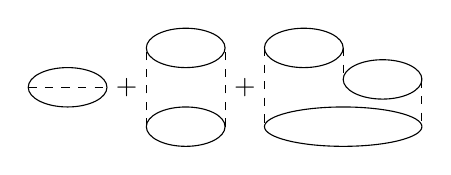
\begin{tikzpicture}
        \draw (0,0) ellipse (0.5 and 0.25);
        \draw [dashed] (-0.5,0)--(0.5,0);
        \node at (0.75,0) {$+$};
        \draw (1.5,0.5) ellipse (0.5 and 0.25);
        \draw (1.5,-0.5) ellipse (0.5 and 0.25);
        \draw [dashed] (1,-0.5)--(1,0.5);
        \draw [dashed] (2.,-0.5)--(2.,0.5);
        \node at (2.25,0) {$+$};
        \draw (3.,0.5) ellipse (0.5 and 0.25);
        \draw (4.,0.1) ellipse (0.5 and 0.25);
        \draw (3.5,-0.5) ellipse (1 and 0.25);
        \draw [dashed] (2.5,0.5)--(2.5,-0.5);
        \draw [dashed] (4.5,0.1)--(4.5,-0.5);
        \draw [dashed] (3.5,0.5)--(3.5,0.1);
    \end{tikzpicture}
    \caption{Link cluster diagram.}%
    \label{fig:3.9}
\end{figure}
They can be summed to give an approximate simple answer.
The rules for constructing diagrams for the terms in the thermodynamic potential are similar to those in Sec~\ref{s3.4}.
One follows all those rules and then multiplies the result by $\frac{\beta}{l}$.
The $ \frac{1}{l} $ factor is just the one which occurs in \eqref{3.265}.
For the first bubble in Fig.~\ref{fig:3.9},
\begin{equation}
    U_2 = \frac{\beta}{2} \frac{\lambda^2}{\beta} \sum_{\bq,iq_n} M^2_\bq \cd^0(\bq,iq_n) P^1(\bq,iq_n)   \label{3.280}
\end{equation}
where the polarization diagram $P^1(\bq,iq_n)$ is for the single bubble, which was already evaluated
\begin{equation}
    P^1(\bq,iq_n) = \frac{2}{\beta V} \sum_{\bp,ip_m} \cg^0(\bp,ip_m) \cg^0(\bp+\bq,ip_m+iq_n)  \label{3.281}
\end{equation}
The second term in Fig.~\ref{fig:3.9} has two bubbles connected by two phonon lines. Using the rules for constructing diagrams gives
\begin{equation}
    U_4 = \frac{\beta}{4} \frac{\lambda^4}{\beta} \sum_{\bq,iq_m} \left[ M_\bq^2 \cd^0(\bq,iq_n) \mathcal{P}^1(\bq,iq+n) \right]^2  \label{3.282}
\end{equation}
Momentum and frequency conservation requires both phonons to have the same variables $(\bq,iq_n)$ and both polarization diagrams are also just functions of combination.
The term with $n$ bubbles and $n$ phonon lines is
\begin{equation}
    U_{2n} = \frac{\beta}{2n} \frac{\lambda^{2n}}{\beta} \sum_{\bq,iq_n} \left[ M^2_\bq \cd^0(\bq,iq_n) \mathcal{P}^1(\bq,iq_n) \right]^n   \label{3.283}
\end{equation}
It is simple to sum the series
\begin{equation}
    \Omega - \Omega_0 = - \frac{1}{\beta} \sum_{n=1}^\infty U_{2n} = \frac{1}{2\beta} \sum_{\bq,iq_n} \ln \left[ 1-\lambda^2 M^2_\bq \cd^0(\bq,iq_n) \mathcal{P}^1(\bq,iq_n)  \right]        \label{3.284}
\end{equation}
This is the correction to the thermodynamic potential.
The right-hand side is proportional to the volume $V$, as is obvious when the summation over $\bq$ is changed to an integration.
The argument of the logarithm is not dependent on $V$, and $V$ enters only by multiplying the result.

The answer in \eqref{3.284} is a logarithm.
The summation over $iq_n$ needs to the evaluated.
A standard trick for eliminating the logarithm, although it does not eliminate it but just disguises it.
Treat $\eta = \lambda^2$ as a variable of integration
\begin{eqnarray}
    &&\int_0^{\lambda^2} d\eta \frac{\Lambda}{1 - \eta\Lambda} = -\ln \left[1 -\lambda^2 \Lambda \right] \label{3.286} \\
    && \Lambda = M^2_\bq \cd^0(\bq,iq_n) \mathcal{P}^1(\bq,iq_n) \label{3.287}
\end{eqnarray}
Then for $\lambda =1$
\begin{equation}
    \Omega- \Omega_0 = - \frac{V}{2\beta} \sum_{iq_n} \int \frac{d^3 q}{(2\pi)^3} \int_0^1 d\eta \frac{M_\bq^2 \cd^0 \mathcal{P}^1}{1 - \eta M^2_\bq \cd^0 \mathcal{P}^1} \label{3.288}
\end{equation}
The logarithm has been eliminated, but now the right-hand side must be evaluated for each value of $\eta$ and then the integral is taken over $\eta$.
\textit{Since $\eta$ enters in the same way as a coupling constant}, this step is called a \textbf{coupling constant integration}.
The integration can be taken outside of the summation over $iq_n$, which makes this summation easier in some case.

Further, define the phonon self-energy as
\begin{equation}
    \pi^1(\eta,\bq,iq_n) = \eta M^2_\bq \mathcal{P}^1(\bq,iq_n) \label{3.289}
\end{equation}
where the coupling constant $\eta$ is included in the definition.
The superscript indicates that this expression is an approximate self-energy, which only includes the single-electron bubble.
The phonon Green's function is
\begin{equation}
    \cd^1(\eta,\bq,iq_n) = \frac{\cd^0}{1-\cd^0 \pi^1}  \label{3.290}
\end{equation}
The Green's function is also a function of the coupling constant strength $\eta$.
Equation \eqref{3.288} is rewritten as
\begin{equation}
    \Omega - \Omega_0 = - \frac{V}{2\beta} \sum_{iq_n} \int \frac{d^3q}{(2\pi)^3} \int_0^1 \frac{d \eta}{\eta} \pi^{(1)}(\eta,\bq,iq_n) \cd^{(1)}(\eta,\bq,iq_n)    \label{3.291}
\end{equation}
This expression is an approximation to $\Omega$ since it employs an approximate self-energy $\pi^{(1)}$.
According the \cite{abrikosov1963methods}, the exact correction to the themodynamic potential from electron-phonon interactions is
\begin{equation}
    \Omega - \Omega_0 = - \frac{V}{2\beta} \sum_{iq_n} \int \frac{d^3q}{(2\pi)^3} \int_0^1 \frac{d \eta}{\eta} \pi(\eta,\bq,iq_n) \cd(\eta,\bq,iq_n)    \label{3.292}
\end{equation}
where $\pi(\eta,\bq,iq_n)$ is the exact phonon self-energy and $\cd(\eta,\bq,iq_n)$ is the exact phonon Green's function evaluated withe excat self-energy.
\begin{figure}[ht]
    \centering
    \includegraphics[width=0.8\linewidth]{fig/fig3-10.jpg}
    \caption{The exact phonon self-energy $\pi(\eta,\bq,iq_n)$ is the summation of this infinite number of diagrams. There are bubbles with internal phonon lines and also several bubbles connected by more then on phonon line.}%
    \label{fig:3.10}
\end{figure}

If electron-electron interactions are included, then the phonon self-energy can also contain internal Coulomb interactions, etc.
The effect of Coulomb interaction on the thermodynamic potential should also be included.
THe general theorem \eqref{3.265} and \eqref{3.266} is true for all interactions: Coulomb, phonon, or others.

It is possible to combine the effects of phonons and Coulomb interaction in a simple way.
Consider electrons interacting by either or both interactions, and then the single-bubble diagram appears twices.
The two electron vertives can be connected by a single Coulomb line or a single phonon line. The sum of these contributions is

It is possible to combine the effects of phonons and Coulomb interaction in a simple way.
Consider electrons interacting by either or both interactions, and then the single-bubble diagram appears twices.
The two electron vertives can be connected by a single Coulomb line or a single phonon line. The sum of these contributions is
\begin{equation}
    U_2 = \frac{\eta}{2} \sum_{\bq,iq_n} \mathcal{P}^{(1)}(\bq,iq_n) \left[ M_\bq^2 \cd^{(0)}(\bq,iq_n)\right] \label{3.293}
\end{equation}
By introduce a combined interaction propagator, Coulomb plus phonon, which is
\begin{equation}
    W^{(0)} (\bq,iq_n) = v_q + M_\bq^2 \cd^{(0)}(\bq,iq_n)  \label{3.295}
\end{equation}
with the Dyson equation
\begin{equation}
    W(\bq,iq_n) = \frac{W^{(0)}(\bq,iq_n)}{1-W^{(0)}(\bq,iq_n)\mathcal{P}^{(1)}}     \label{3.296}
\end{equation}
The generalization of \eqref{3.292} to include both Coulomb and phonon effect is
\begin{eqnarray}
    \Omega- \Omega_0 &=& - \frac{V}{2\beta} \sum_{iq_n} \int \frac{d^3 q}{(2\pi)^3} \int_0^1 \frac{d\eta}{\eta} \pi(\eta,\bq,iq_n) W(\eta,\bq,iq_n) \nonumber\\
    &+& \frac{\eta}{2} \int \frac{d^3q}{(2\pi)^3} v_q \label{3.297}
\end{eqnarray}
The first term contains the Coulomb self-energy of an electron interacting with itself, and this unwanted contribution is substracted out in the second term.
The expression \eqref{3.292} is in the expression of phonon self-energies.
It is also posibble to use electron self-energy, considering \eqref{3.272}
\begin{equation}
    U_2 = \frac{\lambda}{2} \sum_{ip_n,\bp,\sigma} cg^{(0)}(\bp,ip_n) \Sigma^{(1)}(\bp,ip_n)    \label{3.298}
\end{equation}
where $\Sigma^{(1)}$ is the electron self-energy from one-phonon processes, which gives
\begin{equation}
    \Sigma^{(1)}(\bp,ip_n) = \frac{1}{\beta V} \sum_{\bq,iq_m} M^2_\bq \cg^{(0)}(\bq+\bp,ip_n+iq_m) \cd^{(0)}(\bq,iq_m)
\end{equation}

These formulas are often used to calculate the ground state energy in the limit of $T\to0$.
There are two limits which are taken: $V\to\infty$ and $T\to0$.
In studying the electron gas, to get the right answer one needs to take the limit of $V\to\infty$ first.
The reverse order omits important terms,
\begin{equation}
    \beta \eta_F(\xi_\bp) \left[ 1-\eta_f(\xi_\bp)\right]   \label{3.300}
\end{equation}
If $V\neq \infty$, then all levels are discrete in finite volume and as $T\to0$ these terms give zero since either $\eta_F$ or $\left[1-\eta_F\right]$ is zero.
However, if one first takes $V\to\infty$, so that the levels are continuous, then the limit $T\to 0$ gives
\begin{equation}
    \lim_{T\to0} \beta eta_F(\xi_\bp)\left[1 -\eta_F(\xi_\bq)\right] = \lim_{T\to0} \frac{d}{d \xi_\bp} \left[ -\eta_F(\xi_\bp) \right] = \delta(\xi_\bp)   \label{3.301}
\end{equation}
There are many terms of this kind in perurbation expansion for the ground state energy of the electron gas.
They are called \textbf{dangerous diagrams}.

Here we show a simple example of evaluating the thermodynamic potntial.
Assume that the onley effect of the phonon self-energy is to change the unperturbed frequencies $\omega_\bq^2$ to a new set of renormalized frequencies $\Omega^2_\bq$.
Since the Green's function is
\begin{equation}
    \cd = \frac{2\omega_\bq}{(i\omega_n)^2 - \omega_\bq^2 - 2\omega_\bq \pi(\bp,i\omega_n)} = \frac{2\omega_\bq}{(i\omega_n)^2 - \Omega_\bq^2} \label{3.302}
\end{equation}
This form for $\cd$ can be accomplished choosing
\begin{equation}
    2\omega_\bq \pi(\eta,\bp,i\omega_n) = \eta(\Omega_\bq^2 - \omega_\bq^2)     \label{3.303}
\end{equation}
The choice \eqref{3.303} is not the only possible one to renormalize the frequencies.
It is the choice one gets by assuming that the change from $\omega_\bq$ to $\Omega_\bq$ is accomplished by the one-bubble polarization diagram given in \eqref{3.289}.
Then the coupling constant $\eta$ enters as just a mulitplicative factor, as shown in \eqref{3.303}.
If further self-energy diagrams are needed to get a good phonon $\pi$, then $\eta$ would enter in a more complicated fashion.
But usually the single-bubble approximation is often adequate.

Consider the \eqref{3.292}, the expression to be evaluated is
\begin{equation}
    \Omega-\Omega_0 = - \frac{1}{2\beta} \sum_{\bq,iq_n} \int_0^1 d\eta \frac{\Omega_\bq^2 -\omega_\bq^2}{(iq+n)^2 -\omega_\bq^2 -\eta(\Omega_\bq^2-\omega_\bq^2)}  \label{3.304}
\end{equation}
Introduce the frequency
\begin{equation}
    \Omega_\eta^2 = \omega^2_\bq + \eta(\Omega_\bq^2 - \omega_\bq^2)    \label{3.305}
\end{equation}
The summation over Matsubara frequencies can be done easily since,
\begin{equation}
    \frac{1}{\beta} \sum_{iq_n} \frac{1}{(iq_n)^2 - \Omega_\eta^2} = \frac{1}{2\Omega_\eta} \cd_\eta(\tau=0) = - \frac{1}{2\Omega_\eta} \left[ 2\eta_B(\Omega_\eta)+1 \right]   \label{3.306}
\end{equation}
Then the evaluaion of \eqref{3.304} is just the coupling constant integral,
\begin{eqnarray}
    &&\Omega-\Omega_0 = \frac{1}{2} \sum_\bq (\Omega_\bq^2 - \omega_\bq^2) \int_0^1 \frac{d\eta}{2\Omega_\eta} \left(1 + \frac{2}{e^{\beta\Omega_\eta}-1}\right) \nonumber \\
    &&= \frac{1}{2} \sum_\bq \left[ \Omega_\eta + \frac{2}{\beta} \ln \left(1-e^{-\beta\Omega_\eta} \right) \right]^{\eta=1}_{\eta=0} \nonumber \\
    &&= \sum_\bq \left[ \frac{1}{2} \left( \Omega_\bq - \omega_\bq \right) + \frac{1}{\beta} \ln \left( \frac{1-\exp (-\beta \Omega_\bq) }{1- \exp(-\beta \omega_\bq)} \right)\right] \label{3.310}
\end{eqnarray}
The right-hand side is the thermodynamic potential from the phonons at the new frequency $\Omega_\bq$ minus the contribution from the phonons at the old frequencies $\omega_\bq$.
When this result is combined with \eqref{3.260} for $\Omega_0$, the terms with $\omega_\bq$ all cancel. THe final answer is
\begin{equation}
    \Omega = -\frac{2V}{\beta} \int \frac{d^3 p}{(2\pi)^3} \ln \left( 1 + e^{-\beta \xi_\bp} \right) + \frac{V}{\beta} \int \frac{d^3 q}{(2\pi)^2} \left[ \frac{1}{2} \beta \Omega_\bq + \ln\left( 1-e^{-\beta \Omega_\bq}  \right) \right]      \label{3.311}
\end{equation}

\section{Real-Time Green's Function} \label{s.3.7}
For six different Green's function of time, the retarded and advanced function have been discussed at nonzero temperature.
The usefulness of the real-time functions is in the treatment of non-equilibrium phenomena.

The Matsubara method is unsuitable for the non-equilibrium since there is no thermodynamic basis for a system out of equilibrium.
The entire Matsubara method is based on temperature, and no method has been found so far for extending it to nonequilibrium processes.

The real-time functions at nonzero temperature have formal definitions very similar to those at zero temperature.
Comparing with \eqref{2.144}, the Green's functions for electrons of momentum $\bp$ are
\begin{eqnarray}
    \cg^<(\bp,t_1,t_2) &=& i\langle C^\dagger_{\bp\sigma}(t_2) C_{\bp\sigma}(t_1) \rangle \nonumber \\
    \cg^>(\bp,t_1,t_2) &=& -i\langle C_{\bp\sigma}(t_1) C_{\bp\sigma}^\dagger(t_2) \rangle \nonumber \\
    \cg_t(\bp,t_1,t_2) &=& \Theta(t_1-t_2) \cg^>(\bp,t_1,t_2) + \Theta(t_2-t_1) \cg^<(\bp,t_1,t_2) \nonumber \\
    \cg_{\bar{t}}(\bp,t_1,t_2) &=& \Theta(t_2-t_1) \cg^>(\bp,t_1,t_2) + \Theta(t_1-t_2) \cg^<(\bp,t_1,t_2)  \label{3.322}
\end{eqnarray}
These definitions appear to be identical to those at zero temperature.
The definition of $\langle \dots \rangle$ have different meanings, depending on the circumstance:
\begin{itemize}
    \item At zero temperature, and in equilibrium, $\langle \dots \rangle$ denote the ground state of the interacting system
    \item At nonzero temperature, and in equilibrium, the brackets denote the thermodynamic average as in \eqref{3.25} and \eqref{3.82}
    \item When not in equilibrium, the brackets denote an average over the accessible phase space. However, the available phase space depends upon the recent history of the system, and kinetic constrains such as energy conservation. The meaning of brackets is poorly understood for system out of equilibrium.
\end{itemize}
Note in \eqref{3.322} that the Green's functions are not expressed on the difference of the time.
This is only true for equilibrium system.

In thermal equilibrium, the real-time functions each have a simple relation to the retarded function.
Using the state $\ket{n}$ and $\ket{m}$, which are exact eigenstates of the Hamiltonian, we have\footnote{P120 and P155 in Mahan's book}
\begin{eqnarray}
    \cg^<(\bp,\omega) &=& i\eta_F(\omega) A(\bp,\omega) \label{3.325} \\
    \cg^>(\bp,\omega) &=& - i \left[ 1-\eta_F(\omega) \right] A(\bp,\omega) \label{3.326} \\
    \cg_t(\bp,\omega) &=& \left[ 1-\eta_F(\omega)\right] \cg_{ret}(\bp,\omega) + \eta_F(\omega) \cg_{adv}(\bp,\omega) \label{3.327} \\
    \cg_{\bar{t}} (\bp,\omega) &=& -\left[1-\eta_F(\omega)\right] \cg_{adv}(\bp,\omega) - \eta_F(\omega) \cg_{ret}(\bp,\omega) \label{3.328}
\end{eqnarray}
These expression are identical to \eqref{2.160}.

The primary usefulness of the real-time Green's functions is in the theory of non-equilibrium phenomena.
The Dyson's equation is same as the result in zero temperature in \eqref{2.157}, and the matrices have the definition as in \eqref{2.156}.
\marginnote{The \eqref{2.156},
    \begin{eqnarray}
        \tilde{G} =
        \begin{bmatrix}
            G_t & -G^<\\
            G^> & -G_{\bar{t}}
        \end{bmatrix}
        ~ ~ ~ ~
        \tilde{\Sigma} =
        \begin{bmatrix}
            \Sigma_t & -\Sigma^< \\
  \Sigma^> & -\Sigma_{\bar{t}}
  \end{bmatrix} \nonumber
\end{eqnarray}
and \eqref{2.157}
\begin{eqnarray}
    \tilde{G}(x_1,x_2) &=& \tilde{G}_0(x_1-x_2) \nonumber\\
    &+& \int_{-\infty}^\infty dx_3 \int_{-\infty}^\infty dx_4 \tilde{G}_0(x_1-x_3) \nonumber \\
    &\times& \tilde{\Sigma}(x_3,x_4) \tilde{G}(x_4,x_2) \nonumber
\end{eqnarray}
we use the $\tilde{tilde}$ to note this is a matrix.
}

Equation \eqref{2.157} is generally regarded as being the correct form for Dyson's equation, even for systems out of equilibrium.
For systems in equilibrium, one can derive \eqref{2.157} at nonzero temperature by starting from Dyson's equation for the Matsubara Green's functions.
Treating $\tau$ as a complex variable, on can deform the contour of integration, and end up with \eqref{2.157} \cite{Langreth1976}.
Generally, \eqref{2.157} is used for Dyson's equation for nonzero temperature, for equilibrium and nonequilibrium, since there is nothing else available.

Nonequilibrium theory usually proceeds by deriving equations of motion for the Green's function, which is similar to Boltzmann equation.
The first step is to find an equation of motion for the interacting Green's function when it is not in equilibrium.
Such an equation can be found from \eqref{2.157} by operating by $\left(i \frac{\partial}{\partial t} -H \right)$ on both sides of equation.
By the form \eqref{2.144} and \eqref{2.148}, we have (by noting $\tilde{G}$ and the matrix form)
\begin{eqnarray}
    \left( i \frac{\partial}{\partial t} - \varepsilon_\bk \right) \tilde{G}_0 (\bk,t)  &=& \delta(t) \tilde{I}     \label{3.329} \\
    \left( i \frac{\partial}{\partial t} - H_0(x) \right) \tilde{G}_0(x) &=& \delta^4(x) \tilde{I}      \label{3.330}
\end{eqnarray}
On the right-hand side of \eqref{2.157}, this operator acts only upon $\tilde{G}_0$ for which the above result is used to find
\begin{equation}
    \left( i \frac{\partial}{\partial t} - H_0(x) \right) \tilde{G}(x_1,x_2) = \delta^4(x_1-x_2) \tilde{I} + \int dx_3 \tilde{\Sigma}(x_1,x_3) \tilde{G}(x_3,x_2)       \label{3.331}
\end{equation}
This formula provides the equation of motion for the interacting Green's function.
\textbf{It is the basis for the nonequilibrium theory of interacting systems}.
For \eqref{3.331}, on the left-hand side, only the noninteracting terms are contained in the Hamiltonian $H_0$.
The contribution from the interactions is provided by the self-energy functions on the right-hand side.

It is useful to have an equation of motion for the variable $x_2$.
Since the definition \eqref{2.144} of the Green's functions contains the conjugate wave function $\phi^\dagger(x_2)$, the equation of motion on this variable is the complex conjugate of Schrodinger's equation.
Further, Dyson's equation can be written in an alternate form
\begin{equation}
    \tilde{G}(x_1,x_2) = \tilde{G}_0(x_1-x_2) + \int dx_3 \int dx_4 \tilde{G}(x_1,x_3) \tilde{\Sigma}(x_3,x_4) \tilde{G}_0 (x_4-x_2)
\end{equation}
and the alternate equation of motion for the Green's function
\begin{equation}
    \left( -i \frac{\partial}{\partial t}  - H_0(\mathbf{r}_2,-\bp_2) \right) \tilde{G}(x_1,x_2) = \delta^4(x_1-x_2) \tilde{I} + \int dx_3 \tilde{G}(x_1,x_3) \tilde{\Sigma}(x_3,x_2)   \label{3.332}
\end{equation}
The sign change on $\mathbf{p}_2$ comes from the complex conjugate of Schrodinger's equation.
The operator $\mathbf{p}=-i\nabla$ changes sign under complex conjugation.
This behavior is different from the Hermitian conjugate, where $H_0$ acts to the left on $\phi^\dagger(x_2)$ and $\mathbf{p}$ does not change sign.
These two equations of motion will be used to develop a quantum Boltzmann equation for nonequilibrium phenomena.

\subsection{Wigner Distribution Function}
The traditional Boltzmann equation is expressed in terms of the distribution function $f(\mathbf{r},\mathbf{v},t)$.
This is the semiclassical view since it is assumed that the position and velocity of the particle can be defined simultaneously.
In order to use the distribution for quantum systems, it is necessary  to perform some averaging in order to remove effects due to the uncertainty principle.

If quantum effects are important, it is necessary to introduce another variable into the distribution function.
This is called \textbf{Wigner distribution function} $f(\bk,\omega;\mathbf{r},t)$.
This distribution function is derived from the Green's function $G^<(x_1,x_2)$ defined in \eqref{2.144}.
The Wigner distribution is derived by center-of-mass coordinate system
\begin{eqnarray}
    (\mathbf{R},T) &=& \frac{1}{2} (x_1+x_2)  \label{3.333} \\
    (\br,t) &=& x_1 -x_2 \label{3.334}
\end{eqnarray}
with this notation
\begin{equation}
    G^<(\br,t; \mathbf{R},T) = i \langle \psi^\dagger(\mathbf{R}- \frac{1}{2} \br, T- \frac{1}{2} t) \psi(\mathbf{R}+ \frac{1}{2} \br,T + \frac{1}{2} t) \rangle      \label{3.335}
\end{equation}
with Fourier transformation
\begin{equation}
    f(\bk,\omega;\mathbf{R},T) = -i G^<(\bk,\omega;\mathbf{R},T)       \label{3.337}
\end{equation}
For the macroscopic quantities of particle density, particle current and energy density
\begin{eqnarray}
    n(\mathbf{R},T) &=& \int \frac{d^3 k}{(2\pi)^3} \int_{-\infty}^\infty \frac{d\omega}{2\pi}  f(\bk,\omega;\mathbf{R},T) \\
    j(\mathbf{R},T) &=& \int \frac{d^3 k}{(2\pi)^3} \frac{\bk}{m} \int_{-\infty}^\infty \frac{d\omega}{2\pi}  f(\bk,\omega;\mathbf{R},T) \label{3.338} \\
 n_E(\mathbf{R},T) &=& \int \frac{d^3 k}{(2\pi)^3} \int_{-\infty}^\infty \frac{d\omega}{2\pi} \omega f(\bk,\omega;\mathbf{R},T) \nonumber \\
    &=&i\left[ \frac{\partial}{\partial t} \langle \psi^\dagger(\mathbf{R},T- \frac{1}{2} t) \psi(\mathbf{R},T+ \frac{1}{2} t) \rangle \right]_{t=0} \nonumber \\
    &=& \langle \psi^\dagger(\mathbf{R},T) H \psi(\mathbf{R},T) \rangle     \label{3.339}
\end{eqnarray}
Then the technique for solving nonequilibrium problems is simple.
The equation of motion in \ref{3.331} and \ref{3.332} for $G^<(\bk,\omega;\mathbf{R},T)$ is just the \textbf{quantum Boltzmann equation}.
With solving the equations, the Wigner distribution function is yielded and the macroscopic variables can be calculate by the integrals above.\footnote{The current is 0 if the system in equilibrium state, since a system carrying current in steady state but not in equilibrium state.}

The semiclassical Boltzmann distribution function $f(\mathbf{R},\mathbf{v},T)$ is found by taking the frequency integral
\begin{equation}
    f(\mathbf{R},\mathbf{v},T) = \int_{-\infty}^\infty \frac{d \omega}{2\pi} f(m\mathbf{v},\omega;\mathbf{R},T)     \label{3.340}
\end{equation}
This method of deriving the semiclassical Boltzmann equation is an alternative to the usual technique of \textbf{coarse grain averaging}.

The matrix equation in \eqref{3.331} and \eqref{3.332} can be untangled to present the individual equation of motion for separate Green's function.\footnote{P159}

The Wigner density function is not positive definite and can not interpreted as a probability density.
This feature can be shown by a simple example, a particle in one dimensional box of length $L$.
The eigenvalues and eigenfunction are
\begin{eqnarray}
    &&\phi_n(x) = \sqrt{ \frac{2}{L} } \sin(k_n x), ~ ~ \varepsilon_n = \varepsilon n^2 \label{3.343} \\
    && k_n = \frac{n\pi}{L} , ~ ~ \varepsilon = \frac{\pi^2}{2mL^2}  \label{3.344}
\end{eqnarray}
Using the representation in \eqref{2.147} and setting $t = t_1 -t_2$, gives
\begin{equation}
    G^<(x_1,x_2,t) = \frac{2i}{L} \sum_n \eta_F(\varepsilon_n) \sin(k_n x_1) \sin(k_nx_2) e^{-it \varepsilon n^2}   \label{3.345}
\end{equation}
With the Fourier transform of time gives the function of frequency.
Since the system is equilibrium, write $G^< = i\eta_F(\omega)A$.
In the center-of-mass notation
\begin{eqnarray}
    f(x,\omega;X) &=& \eta_F(\omega) A(x,\omega;X)  \label{3.346} \\
    A(x,\omega;X) &=& \frac{2\pi}{L} \sum_n \left[ \cos(k_n x) - \cos(2k_n X) \right] \delta(\omega-\varepsilon n^2)    \label{3.347}
\end{eqnarray}
where $x= x_1-x_2$ and $X= (x_1+ x_2)/2$.
The function $A$ is a sum of delta function with different sign.

\section{Kubo Formula For Electrical Conductivity} \label{s3.8}
Many Experiments in condensed matter physics measure the linear response to an external perturbation.
Linear response means that the signal is directly proportional to the intensity of the external perturbation.
Kubo formulas are the name applied to the correlation function which describes the linear response.

For conductivity response, as an example, the applied or external field $E_\alpha^{ext}$ induces currents which in turn make other electric fields.
The summation of all these fields is the total electric field, which is called $E_\alpha(\br,t)$.
The conductivity $\sigma$ is the one which responds tot he actual electric field in solid
\begin{eqnarray}
    J_\alpha (\br,t) &=& \sum_\beta \sigma_{\alpha\beta} (\bq,\omega) E_\beta(\br,t)    \label{3.350} \\
    E_\alpha (\br,t) &=& \Xi_\alpha \exp \left[ i(\bq \br - \omega t)  \right]   \label{3.351}
\end{eqnarray}
Take \eqref{3.350} as the fundamental definition of the microscopic conductivity.
And implies the spacetime response as
\begin{equation}
    J_\alpha (\br,t) = \int d^3 \br' \int_{-\infty}^t dt' \sigma_{\alpha\beta}(\br-\br',t-t') E_\beta (\br',t')     \label{3.352}
\end{equation}
In solids, it is permissible to use \eqref{3.350} only when it is understood that the current is to be averaged over many unit cells of the solid.
Usually it is applied when $\bq$ is small and long-wavelength excitations are being studied.

Considering the dc conductivity, where $\bq\to 0$ and $\omega \to 0$ and assuming that the system is linear and perturbations at different frequencies act independently.
Then the total current is the summation of the responses at different frequencies.

The Hamiltonian for the system is taken to have $H+H'$.
The term $H'$ contains the interaction between the total electric field and the particles of the system.
Equation \eqref{2.161} is used as the basic form of the interaction between electromagnetic fields and charges, in the expression of vector potential
\begin{eqnarray}
    H' &=& - \frac{1}{c} \int d^3 r j_\alpha(\br) A_\alpha (\br,t)    \label{3.354} \\
    \frac{1}{c} A_\alpha (\br,t) &=& - \frac{i}{\omega} E_\alpha (\br,t)    \label{3.355}
\end{eqnarray}
with the Coulomb gauge $\nabla \cdot \mathbf{A} = 0$, also the electric and vector potential are taken to be transverse, so the scalar potential $\phi$ is set equal to zero.
The terms in \eqref{2.161} with $A^2$ are dropped, since their effects are nonlinear in the electric field.
\footnote{ The equation \eqref{2.161}
\begin{equation}
      H=\sum_i \frac{1}{2m}[\bp_i - \frac{e}{c} \mathbf{A}(\br_i)]^2 + \frac{1}{2} \sum_{i\neq j}\frac{e_i e_j}{r_{ij}} + \sum_{\bk \lambda} \omega_{\bk \lambda} a^\dagger_{\bk \lambda} a_{\bk \lambda} \nonumber
\end{equation}
}
The term $H$ contains all the other terms and interactions in the solid or liquid.
There are interactions such as electron-electron, electron-phonon, spin-spin, with impurities, etc.
The goal is to calculate the electrical conductivity when all these interactions are present.

The current operator in \eqref{3.354} was discussed earlier in Chapter one.
\begin{equation}
    j_\alpha = \frac{1}{2m} \sum_i e_i \left[ \bp_{i\alpha} \delta(\br-\br_i) + \delta(\br- \br_i) \bp_{i\alpha}  \right] \label{3.356}
\end{equation}
With \eqref{3.351}, \eqref{3.354} and \eqref{3.355} we have
\begin{eqnarray}
    H' &=& \frac{i}{\omega} j_\alpha (\bq) \Xi_\alpha e^{-i\omega t}    \label{3.357} \\
    j_\alpha (\bq) &=& \frac{1}{2m} \sum_i e_i \left[ \bq_{i\alpha} e^{i\bq \br_i} + e^{i \bq \br_i} \bp_{i\alpha}  \right]     \label{3.358}
\end{eqnarray}
In terms of creation and destruction operators, the current operator is conventionally written as
\begin{equation}
    j_\alpha (\bq) = \sum_{\lambda \delta} p_\alpha^{\lambda \delta} C^\dagger_\lambda C_\delta     \label{3.359}
\end{equation}
where $\lambda, \delta$ are the states associated with some unperturbed Hamiltonian $H_0$ which is chosen as the basis for the perturbation expansion.
A distinction is make between the current operator $j_\alpha$ in \eqref{3.358} and the induced current $J_\alpha$ in \eqref{3.350}.
The operator $j_\alpha$ is used in the Hamiltonian, while $J_\alpha$ is the actual current measured by experiment.
The measured value of the current is the average value for the velocity of the particles in the system, which is taken as the summation over all the particle velocities divided by the volume
\begin{equation}
    J_\alpha(\br,t) = \frac{e}{V} \langle \sum_i v_{i\alpha} \delta(\br-\br_i) \rangle = \frac{e}{V} \sum_i \langle v_{i\alpha} \rangle     \label{3.360}
\end{equation}
When quantizing the particle velocity in \eqref{1.410}, the velocity is momentum minus the vector potential
\begin{eqnarray}
    \mathbf{v}_i &=& \left[ \mathbf{p}_i - \frac{e}{c} \mathbf{A}(\br_i) \right]    \label{3.361} \\
    J_\alpha &=& \frac{e}{mV} \sum_i \langle p_{i\alpha} \rangle - \frac{e^2}{mcV} \sum_i A_\alpha (\br_i)  \label{3.62}
\end{eqnarray}
The momentum operator $\mathbf{p}_i$ is proportional to the current operator, $\mathbf{j} = e \frac{\mathbf{p}_i}{m} $.
The last term uses the relationship \eqref{3.355} between the vector potential and the electric field.
For the long-wavelength disturbance
\begin{equation}
    J_\alpha (\br,t) = \langle j_\alpha (\br,t) \rangle + i \frac{n_0 e^2}{m\omega} E_\alpha(\br,t) \label{3.363}
\end{equation}
The second term in the current is proportional to the electric field and the first term given by the expectation value of the local current operator.
Later it is shown that the constant of proportionality is given by the Kubo formula.
Usually these two terms are called
\begin{eqnarray}
    \mathbf{J} &=& \mathbf{J}^{(1)} + \mathbf{J}^{(2)}    \label{3.364} \\
    \mathbf{J}^{(1)} &=& \frac{in_0 e^2}{m\omega} \mathbf{E}( \br,t)    \label{3.365} \\
    \mathbf{J}^{(2)} &=& \langle \mathbf{j}(\br,t) \rangle  \label{3.366}
\end{eqnarray}

\subsection{Transverse Fields, Zero Temperature}
The following derivation of the Kubo formula is valid at zero temperature.
Consider the expectation value of the current operator as a function of time
\begin{equation}
    J_\alpha^{(2)}(\br,t) = \bra{\psi'} e^{i(H+H')t} j_\alpha(\br) e^{-i(H+H')t}  \ket{\psi}    \label{3.367}
\end{equation}
The \textbf{Heisenberg representation} is used here, as explained in \ref{s2.2}.
Next go to the interaction representation, where $H'$ is treated as the perturbation.
\begin{eqnarray}
    e^{-i(H+H')t} &=& e^{-itH}U(t)  \label{3.368}   \\
    U(t) &=& e^{itH} e^{-i(H+H')t}  \label{3.369}   \\
    J^{(2)}_\alpha (\br,t) &=& \bra{\psi'} U^\dagger(t) e^{itH} j_\alpha(\br) e^{-itH} U(t) \ket{\psi'}  \label{3.370}
\end{eqnarray}
The operator $U(t)$ was defined in \eqref{2.14} and with a formal solution in \eqref{2.27} where the usual definitions are
\begin{eqnarray}
    H'(t) &=& e^{itH} H' e^{-itH}   \label{3.372}   \\
    j(t) &=& e^{itH} j e^{-itH},~ etc     \label{3.373}
\end{eqnarray}
The wave function $\ket{\psi'}$ in \eqref{3.367} is the Schr{\"o}dinger wave function at $t=0$ for an interacting system with both $H+H'$ as the Hamiltonian.
As discussed in Sec.\ref{s3.1}, the wave function $\ket{\psi}$ is accurate when $H'$ is absent.
Using the relation \eqref{2.36}
\begin{equation}
    \ket{\psi'} = T \exp \left[ -i \int_{-\infty}^0 dt' H'(t') \right] \ket{\psi}    \label{3.374}
\end{equation}
Then the time development of the system is given by combining these result
\begin{equation}
    U(t) \ket{\psi'} = T \exp \left[ -i \int_{-\infty}^t dt' H'(t') \right] \ket{\psi} = S(t,-\infty) \ket{\psi}    \label{3.376}
\end{equation}
The expectation value of the current is
\begin{equation}
    J_\alpha^{(2)} = \bra{\psi} S^\dagger(t,-\infty) j_\alpha(\br,t) S(t,-\infty) \ket{\psi}    \label{3.377}
\end{equation}
For Kubo formula, only terms linear in $H'$ is required, then
\begin{equation}
    S(t,-\infty) \ket{\psi} = \left[ 1 - i \int_{-\infty}^t d t' H'(t') \right] \ket{\psi} + O(H')^2    \label{3.379}
\end{equation}
From \eqref{3.377}, we have the expectation value of the current operator.
The first term is assumed to vanish
\begin{equation}
    \bra{\psi} j_\alpha(\br,t) \ket{\psi} = 0       \label{3.380}
\end{equation}
since there is usually no current in the solid in the absence of an electric field.
The first nonzero term is the one linear in $H'$, which is the important contribution, and can be expressed as commutator
\begin{equation}
    J_\alpha^{(2)} (\br,t) = -i \int_{-\infty}^t dt' \bra{\psi} \left[ j_\alpha(\br,t), H'(t') \right] \ket{\psi}       \label{3.381}
\end{equation}
With $H'$ given in \eqref{3.358}, the integrand have
\begin{eqnarray}
    \left[ j_\alpha(\br,t), H'(t') \right] &=& \frac{i}{\omega} \Xi_\beta e^{-i \omega t'} \left[j_\alpha(\br,t), j_\beta(\bq,t') \right] \label{3.382}\\
    &=& \frac{i}{\omega} E_\beta(\br,t) e^{-i \bq \br} e^{i\omega(t-t')} \left[ j_\alpha(\br,t) , j_\beta(\bq,t')\right]   \nonumber
\end{eqnarray}
Comparing the result with \eqref{3.350} shows that
\begin{equation}
    \sigma_{\alpha\beta} = \frac{1}{\omega} e^{-i\bq\br} \int_{-\infty}^t dt' e^{i\omega(t-t')} \bra{\psi} \left[ j_\alpha(\br,t),j_\beta(\bq,t')\right] \ket{\psi} + i \frac{n_0 e^2}{m\omega} \delta_{\alpha\beta}    \label{3.383}
\end{equation}
The final step is to average over the space variable $\br$ in order to eliminate atomic fluctuations.
Take this average by integrating over all volume $d^3r$ and then divide by $V$.
Take the $r$ dependence of the expression\footnote{Not Fourier transformation, check \eqref{3.356} and \eqref{3.358}.}
\begin{equation}
    \int d^3 r e^{-i\bq \br} j_\alpha(\br,t) = j_\alpha(-\bq,t) = j_\alpha^\dagger(\bq,t)   \label{3.384}
\end{equation}
Then by change the notation of $t$, the Kubo formula
\begin{equation}
    \sigma_{\alpha\beta}(\bq,\omega) = \frac{1}{\omega V} \int_0^\infty dt e^{i\omega t} \bra{\psi} \left[j^\dagger_\alpha(\bq,t),j_\beta(\bq,0) \right] \ket{\psi} + i \frac{n_0 e^2}{m\omega} \delta_{\alpha \beta}   \label{3.385}
\end{equation}

The wave function $ket{\psi}$ in \eqref{3.385} is the ground state of the many-body Hamiltonian $H$, which contains all the possible interaction in the solid except the interaction with the vector potential $H'$.
In \eqref{3.385}, the conductivity has no mention of photon field, since conductivity is an intrinsic property of the ground state of the system.
Equation \eqref{3.350} can be viewed as a Taylor series in the applied electric field
\begin{equation}
    J_\alpha(\Xi_\beta) = J_\alpha(0) + \left( \frac{\partial J_\alpha}{\partial \Xi_\beta} \right) \Xi_\beta^{(ext)} + O^2 \label{3.386}
\end{equation}
Where the conductivity is $\sigma_{\alpha\beta} = (\partial J_\alpha /\partial \Xi_\beta)$.
It is a characteristic of all linear response correlation functions that they are ground state properties.

The Kubo formulas contain a retarded, two-particle correlation function.
The retarded correlation function the current operator based on \eqref{3.88}
\begin{equation}
    \Pi_{\alpha\beta}(\bq,t-t') = - \frac{i}{v} \theta(t-t') \bra{\psi} \left[j^\dagger_\alpha(\bq,t),j_\beta(\bq,t') \right] \ket{\psi}    \label{3.387}
\end{equation}
With Fourier transformation,
\begin{equation}
    \Pi_{\alpha\beta}(\bq,\omega) = - \frac{i}{v} \int_{-\infty}^\infty dt e^{i\omega(t-t')} \theta(t-t') \bra{\psi} \left[j^\dagger_\alpha(\bq,t),j_\beta(\bq,t') \right] \ket{\psi}
\end{equation}
we have
\begin{equation}
    \sigma_{\alpha\beta}(\bq,\omega) = \frac{i}{\omega} \left[\Pi_{\alpha\beta}(\bq,\omega) + \frac{n_0e^2}{m} \delta_{\alpha\beta} \right] \label{3.388}
\end{equation}
The conductivity is the \textbf{retarded correlation function} of the current multiplied by $i$ and divided by $\omega$.
The correlation function $\Pi_{\alpha\beta}(\bq,\omega)$ is usually called the \textbf{current-current correlation function}.
These quantities usually by the Matsubara method and with analytic extension.

The dc conductivity is obtained by taking the limit $\bq \to 0$ and then the limit $\omega \to 0$.
Be careful that wrong answer may be obtained if the order of these limits is reversed.
\begin{equation}
    \lim_{\bq \to 0}
    \begin{cases}
        \sigma_{\alpha\beta}(\bq,\omega) &= \sigma_{\alpha\beta}(\omega) \\
        \Pi_{\alpha\beta}(\bq,i\omega_n) &= \Pi_{\alpha\beta}(i\omega_n) \\
        \Pi_{\alpha\beta}(\bq,\omega) &= \Pi_{\alpha\beta}(\omega)\\
        j_\alpha(\bq,\tau) &=j_\alpha(\tau)
    \end{cases}
    \label{3.392}
\end{equation}

The limit of $\omega \to 0$ is more delicate.
Here the conductivity is real,
\begin{equation}
    \Re \sigma_{\alpha\beta} = - \lim_{\omega\to 0} \frac{1}{\omega} \Im \left[\Pi_{\alpha\beta}(\omega) \right]    \label{3.393}
\end{equation}
The right-hand side contains the imaginary part of the retarded correlation function which is related to the spectral function of that operator.
One thing is that \eqref{3.385} is the right Kubo formula at nonzero temperatures.

The current-current correlation function is a \textbf{two-particle correlation function}.
This correlation function describes how two particles are created and destroyed.
The conductivity arises from correlations between these two events.
Measure quantities always involve retarded correlation functions of at least two particles.
The one-particle Green's function can never be measured in the rigorous sense, since real particles cannot be created or destroyed.

The two-particle correlation function, wherein a particle changes its state, is always found in the correlation functions of linear response.
In elementary particle physics, a particle can be absolutely destroyed or created.
But this event always happens in conjunction with some other event which involves other particles.
For example,and electron and positron can mutually annihilate and make several photons.
Then one would have terms in the current operator involving the creation or destruction of two particles
\begin{equation}
    j_\alpha(\bq) = \sum \left[ p_\alpha^{(\lambda\delta)} C_\lambda d_\delta + h.c. \right]    \label{3.399}
\end{equation}
If the particles interact, then the correlation function may not be divided into two independent Green's function
\begin{equation}
    \langle T_\tau C_\lambda(\tau) d_\delta(\tau) d^\dagger_\delta(0) C^\dagger_\lambda(0)\rangle \neq \langle T_\tau C_\lambda(\tau) C^\dagger_\lambda(0) \rangle \langle T_\tau d_\delta(\tau) d^\dagger_\delta(0) \rangle    \label{3.400}
\end{equation}
When taking an electron from a filled band and moving it to an empty or partially filled band, then one has a current operator of the form \eqref{3.399}, which is used to describe the electron-hole excitation process.

\subsection{Nonzero Temperature}
As time-varying perturbation $H'(t)$ is put into the system at nonzero temperature.
The central question concerns the degree to which the thermodynamic averaging is influenced by the time-varying interaction.
In Kubo's derivation, the density matrix $\rho_0 = \exp\left[\beta (\Omega-H+\mu N)\right]$ applies to the equilibrium system in the absence of $H'(t)$.
It is assumed that the system is described by the density matrix at the initial point in the time, $t\to -\infty$.
The perturbation $H'$ is \textbf{adiabatically} switched on as the system is brought forward in time to the present.
Now the time-dependent density matrix, have the following result
\begin{eqnarray}
    \frac{d}{dt} \rho(t) &=& -i \left[H + H'(t), \rho(t) \right]    \label{3.406}   \\
    J^{(2)}_\alpha &=& \Tr\left[ \rho(t) j_\alpha \right]   \label{3.407}
\end{eqnarray}
Kubo's staring point is tantamount to not including $H'(t)$ in the thermodynamic weighting factor.
The density matrix is defined as $\rho(t) = \rho_0 + f(t) $, where $\rho_0$ is the density matrix in the absence of $H'$.
The equilibrium density matrix $\rho_0$ is time independent,
\begin{eqnarray}
    i \frac{d}{dt} f &=& \left[ H,\rho_0 \right] + \left[ H,f \right] + \left[ H',\rho_0 \right] + \left[ H', f \right] \label{3.408}   \\
    \left[ H, \rho_0 \right] &=& 0  \label{3.409}
\end{eqnarray}
The objective is to solve for the term in $J^{(2)}$, which is proportional to $H'$, which is treated as infinitesimal.
Since $f$ is proportional to $H'$, it follows that $f$ is small.
Terms proportional to $O(H')^2$, such as $\left[ H', f \right]$ are neglected, then
\begin{equation}
    e^{-itH} \left[ i \frac{d}{dt} (e^{itH} f e^{-itH}) \right] e^{itH} = i \frac{d}{dt} f - \left[ H, f\right] = \left[ H' , \rho_0 \right]    \label{3.412}
\end{equation}
The linear differential equation may be integrated to give
\begin{equation}
    f(t) = -i e^{-itH} \left[ \int_{-\infty}^t dt' \left[ H'(t'), \rho_0 \right] \right] e^{itH}    \label{3.414}
\end{equation}
Then the evaluation of \eqref{3.407} is \footnote{ The derivation in P169 is not so clear to me still}
\begin{equation}
    J^{(2)}_\alpha = \Tr \left[ \rho_0 j_\alpha \right] + \Tr \left[ f(t) j_\alpha \right] \label{3.415}
\end{equation}
The first term is zero, since it is equilibrium.
By changing the terms in the trace, we get the Kubo formula \eqref{3.385}
\begin{equation}
    J^{(2)}_\alpha (\br,t) = -i \int_{-\infty}^t dt' \langle \left[j_\alpha(\br,t),H'(t') \right] \rangle   \label{3.420}
\end{equation}

\chapter{Quantum mecahnics in three dimensions}
\section{Schr\"odinger equation in spherical coordinates}
The generalization to three dimsnison is straightforward.
\begin{equation}
  \label{eq:4-1}
  i\hbar \frac{\partial \Psi}{\partial t} = - \frac{\hbar^{2}}{2m} \nabla^{2} \Psi + V\Psi
\end{equation}
where the \textbf{Laplacion} is
\begin{equation}
  \label{eq:4-2}
  \nabla^{2} \equiv \frac{\partial^{2}}{\partial x^{2}} + \frac{\partial^{2}}{\partial y^{2}} + \frac{\partial^{2}}{\partial z^{2}}
\end{equation}
in cartesian coordinates.
With the separation of the variables the general solution gives
\begin{equation}
  \label{eq:4-3}
  \Psi \left( \mathbf{r},t \right) = \sum c_{n} \psi_{n} \left( \mathbf{r} \right) e^{-i E_{n}t/\hbar}.
\end{equation}

\subsection{Separation of variables}
Typically, the potential is a function only of the distance from the origin.
In that case it is natural to adopt \textbf{spehrical coordinates}, as shown in Fig.~\ref{fig:4-1}, the Laplacian takes the form for our time-independent Schr\"odinger equation
\begin{equation}
  \label{eq:4-4}
  \nabla^{2} = \frac{1}{r^{2}} \frac{\partial }{\partial r} \left( r^{2} \frac{\partial}{\partial r} \right) + \frac{1}{r^{2}\sin\theta} \frac{\partial}{\partial \theta} \left( \sin\theta \frac{\partial}{\partial \theta} \right) + \frac{1}{r^{2} \sin^{2} \theta} \left( \frac{\partial^{2}}{\partial \phi^{2}} \right).
\end{equation}
\begin{figure}[h]
  \centering
  \includegraphics[width=0.45\textwidth]{fig/fig4-1.png}
  \caption{Spherical coordinates.}
  \label{fig:4-1}
\end{figure}

We begin by looking for solutions that are separable into products
\begin{equation}
  \label{eq:4-5}
  \psi \left( r,\theta,\phi \right) = R \left( r \right) Y \left( \theta, \phi \right).
\end{equation}
With this ansatz, we have
\begin{equation}
  \label{eq:4-6}
  \left\{ \frac{1}{R} \frac{\dd}{\dd r} \left( r^{2} \frac{\dd R}{\dd r} \right) - \frac{2mr^{2}}{\hbar^{2}} \left[ V \left( r \right) -E \right] \right\}  + \frac{1}{Y} \left\{  \frac{1}{\sin\theta} \frac{\partial}{\partial \theta} \left( \sin\theta \frac{\partial Y}{\partial \theta} \right) + \frac{1}{ \sin^{2} \theta} \frac{\partial^{2} Y}{\partial \phi^{2}} \right\} = 0
\end{equation}
again each curly bracket should equal to a constant $l \left( l+1 \right)$
\begin{align}
  \label{eq:4-7}
  \left\{ \frac{1}{R} \frac{\dd}{\dd r} \left( r^{2} \frac{\dd R}{\dd r} \right) - \frac{2mr^{2}}{\hbar^{2}} \left[ V \left( r \right) -E \right] \right\} &= l \left( l+1 \right) \\
  \label{eq:4-8}
  \frac{1}{Y} \left\{  \frac{1}{\sin\theta} \frac{\partial}{\partial \theta} \left( \sin\theta \frac{\partial Y}{\partial \theta} \right) + \frac{1}{ \sin^{2} \theta} \frac{\partial^{2} Y}{\partial \phi^{2}} \right\} &= - l \left( l+1 \right).
\end{align}

\subsection{The angular equation}
We first consider Eq.~\eqref{eq:4-8}, which it equals
\begin{equation}
  \label{eq:4-9}
  \sin\theta \frac{\partial}{\partial \theta} \left( \sin\theta \frac{\partial Y}{\partial \theta} \right) + \frac{\partial^{2} Y}{\partial \phi^{2}} = -l \left( l+1 \right) \sin^{2} \theta Y.
\end{equation}
Once again we separate the variables $Y \left( \theta,\phi \right) = \Theta \left( \theta \right) \Phi \left( \phi \right) $.
Equation~\eqref{eq:4-9} can be further separate into two by setting a new constant $m^{2}$
\begin{align}
  \label{eq:4-10}
  \frac{1}{\Theta} \left[ \sin\theta \frac{\dd}{\dd \theta} \left( \sin\theta \frac{\dd \Theta}{\dd \theta} \right) \right] + l \left( l+1 \right) \sin^{2} \theta &= m^{2} \\
  \label{eq:4-11}
  \frac{1}{\Phi} \frac{\dd^{2} \Phi}{\dd \phi^{2}} = - m^{2}
\end{align}
This $\phi$ equation is easy, we have the general solution
\begin{equation}
  \label{eq:4-12}
  \Phi \left( \phi \right) = e^{im\phi}.
\end{equation}
Again we could absorb the canstant into $\Theta$ function.
Since when we rotate $\phi$ by $2\pi$ angle, it back to the same point, it is nature to require that $\Phi \left( \phi + 2\pi \right) = \Phi \left( \phi \right)$.
In other words, we have the constrain such that $\exp \left( 2\pi i m \right)=1$, which means $m$ must be an integer
\begin{equation}
  \label{eq:4-13}
  m = 0, \pm 1, \pm 2, \ldots.
\end{equation}

For the $\theta$ equation in Eq.~\eqref{eq:4-10}, the solution is
\begin{equation}
  \label{eq:4-14}
  \Theta \left( \theta \right) = A P_{l}^{m} \left(\cos \theta \right)
\end{equation}
where $P_{l}^m$ is the \textbf{associated Legendre function}, defined by
\begin{equation}
  \label{eq:4-15}
  P_l^m \left( x \right) \equiv \left( 1-x^2 \right)^{\abs{m}/2} \left( \frac{\dd}{\dd x} \right)^{\abs{m}} P_l \left( x \right) ,
\end{equation}
and $P_l \left( x \right)$ is the $l-$th \textbf{Legendre polynomial}, defined by the \textbf{Rodigures formuale}
\begin{equation}
  \label{eq:4-16}
  P_l \left( x \right) \equiv \frac{1}{2^{l} l!} \left( \frac{\dd}{\dd x} \right)^l \left( x^2 -1 \right)^l.
\end{equation}
Some result of $P_l^m \left( \cos \theta \right)$ is listed in Tab.~\ref{tab:4-1}.
\begin{table}[h]
  \centering
  \begin{tabular}{c c c}
    \toprule
    $P_0^0 = 1$ &  &  \\
    \midrule
    $P_1^0 = \sin \theta$ & $P_1^1= \sin \theta$ & \\
    \midrule
    $P_2^0 = \frac{1}{2} \left( 3 \cos^2 \theta -1 \right)$ & $P_2^1 = 3\sin \theta \cos \theta$ & $P_2^2 = 3 \sin^2\theta$ \\
    \bottomrule
  \end{tabular}
  \caption{Some associated Legendre functions}
  \label{tab:4-1}
\end{table}
Noticee that $l$ must be a nonegation integer because of senseness of the Rodrigues formula in Eq.~\eqref{eq:4-16}.
Moreover, for any $\abs{m}>l$, Eq.~\eqref{eq:4-14} always says $P_l^m=0$.
Then for any given $l$, there are $\left( 2l+1 \right)$ possible value of $m$,\footnote{Notice Eq.~\eqref{eq:4-10} is a second-order differential equation: It should have two linearly independent solutions, for any old values of $l$ and $m$. However the rest of the solution are not physical, because they blow up at $\theta=0, \pi$.}
\begin{equation}
  \label{eq:4-17}
  l = 0, 1, 2, \ldots; ~ ~ m = -l, -l+1, \ldots, -1, 0, 1, \ldots, l-1, l.
\end{equation}

For normalization condition, we have
\begin{equation}
  \label{eq:4-18}
  \int \abs{\psi}^2 r^2 \sin\theta \dd r \dd \theta \dd \phi = \int \abs{R}^2 r^2 \dd r \int \abs{Y}^2 \sin\theta \dd \theta \dd \phi = 1.
\end{equation}
It is convenient to normalize $R$ and $Y$ separately
\begin{equation}
  \label{eq:4-19}
  \int_0^{\infty} \abs{R}^2 r^2 \dd r =1 ~ ~ ~ \text{and} ~ ~ ~ \int_0^{2\pi}\int_0^{\pi} \abs{Y}^2 \sin\theta \dd \theta \dd \phi =1.
\end{equation}
The normalized angular wave functions are called \textbf{spherical harmonics}
\begin{equation}
  \label{eq:4-20}
  Y_l^m \left( \theta,\phi \right) = \epsilon \sqrt{ \frac{\left( 2l+1 \right)}{4\pi} \frac{\left( l-\abs{m} \right)!}{\left( l+\abs{m} \right)!}} e^{im\phi} P_l^m \left( \cos\theta \right),
\end{equation}
where $\epsilon=\left( -1 \right)^{m}$ for $m \geq 0$ and $\epsilon=1$ for $m \leq 0$.
As expected these spherical harmonics function are orthogonal to each other
\begin{equation}
  \label{eq:4-21}
  \int_0^{2\pi} \int_0^{\pi} \left[ Y_l^m \left( \theta,\phi \right) \right]^{*} \left[ Y_{l'}^{m'} \left( \theta,\phi \right) \right] \sin \theta \dd \theta \dd \phi = \delta_{ll'} \delta_{mm'}
\end{equation}
For historical reason, $l$ is called the \textbf{azimuthal quantum number}, and $m$ is the \textbf{magnetic quantum number}.

\subsection{The radial equation}
Notice that the angular part of the wavefunctino, $Y \left( \theta,\phi \right)$, is the same for all spherically symmetric potentials;
The actual shape of the potential affects only the radial part of the wave function, $R \left( r \right)$, which is
\begin{equation}
  \label{eq:4-22}
  \frac{\dd }{\dd r} \left( r^2 \frac{\dd R}{\dd r} \right) - \frac{2mr^{2}}{\hbar^{2}} \left[ V \left( r \right) - E \right] R = l \left( l+1 \right) R.
\end{equation}
One can simplifies this equation if we change the variables
\begin{equation}
  \label{eq:4-23}
  u \left( r \right)  \equiv r R \left( r \right) ,
\end{equation}
and hence we have
\begin{equation}
  \label{eq:4-24}
  - \frac{\hbar^{2}}{2m} \frac{\dd^{2} u}{d r^2} + \left[ V + \frac{\hbar^{2}}{2m} \frac{l \left( l+1 \right)}{r^2} \right] u = Eu.
\end{equation}
This is called the \textbf{radial equation}; it is identical in form to the one-dimentional Schr\"odinger equation Eq.~\eqref{eq:2-5}, except that the \textbf{effective potential},
\begin{equation}
  \label{eq:4-25}
  V_{eff} = V + \frac{\hbar^{2}}{2m} \frac{l \left( l+1 \right)}{r^{2}}.
\end{equation}
Meanwhile the normalization in Eq.~\eqref{eq:4-19} becomes to the form
\begin{equation}
  \label{eq:4-26}
  \int_0^{\infty} \abs{u}^2 \dd r = 1.
\end{equation}
This is as far as we can go before the potential is provoided.

\section{The Hydrogen atom}
The hydrogen atom consists of a heavy motionless proton of charge $e$ together with a light electron that orbits around it.
Forom the Coulomb's law, the potential energy is
\begin{equation}
  \label{eq:4-27}
  V \left( r \right) = - \frac{e^{2}}{4\pi \epsilon_{0}} \frac{1}{r}
\end{equation}
and the radial equation Eq.~\eqref{eq:4-24} reads
\begin{equation}
  \label{eq:4-28}
  - \frac{\hbar^{2}}{2m} \frac{\dd^{2} u}{d r^2} + \left[ - \frac{e^{2}}{4\pi \epsilon_{0}} \frac{1}{r} + \frac{\hbar^{2}}{2m} \frac{l \left( l+1 \right)}{r^2} \right] u = Eu.
\end{equation}
In principle, the Coulomb potential admits continuum sates, (for $ E>0 $ ), describing electron-proton scattering, as wellas discrete bond states, representing the hydrogen atom.
We will focus on the latter case.

\subsection{The radial wave function}
With the new notation\footnote{For bound states, $E$ is negative, so $\kappa$ is real.}
\begin{equation}
  \label{eq:4-29}
  \kappa \equiv \frac{\sqrt{-2mE}}{\hbar},
\end{equation}
then Eq.~\eqref{eq:4-28} reads
\begin{equation}
  \label{eq:4-30}
  \frac{1}{\kappa^{2}} \frac{\dd^{2} u}{\dd r^{2}} = \left[ 1 - \frac{m e^{2}}{2 \pi \epsilon_{0} \hbar^{2} \kappa} \frac{1}{\left(\kappa r\right)} + \frac{l \left( l+1 \right)}{\left( \kappa r \right)^2} \right] u.
\end{equation}
This furter suggests that we have
\begin{equation}
  \label{eq:4-31}
  \rho \equiv \kappa r, ~ ~ ~  \text{and} ~ ~ ~ \rho_0 \equiv \frac{me^{2}}{2\pi \epsilon_{0} \hbar^{2} \kappa},
\end{equation}
so that
\begin{equation}
  \label{eq:4-32}
  \frac{\dd^{2} u}{\dd \rho^{2}} = \left[ 1 - \frac{\rho_{0}}{\rho} + \frac{l \left(l+1\right)}{\rho^{2}} \right] u.
\end{equation}

Let us exame the asymptotic form of the solutions.
As $\rho \to \infty$, the Eq.~\eqref{eq:4-32} can be approximated to
\begin{equation}
  \label{eq:4-33}
  \frac{\dd^{2} u}{\dd \rho^2} = u.
\end{equation}
The general solution is $u \left( \rho \right) = A e^{-\rho} + B e^{\rho}$.
In order to get a finite solution at $\rho \to \infty$, we have to require $B=0$.
So, for large $\rho$ we have
\begin{equation}
  \label{eq:4-34}
  u \left( \rho \right) \sim A e^{-\rho}.
\end{equation}
On the other hand, as $\rho \to 0$ the centrifugal term dominates\footnote{This argument does not apply when $l=0$, although the result we got, Eq.~\eqref{eq:4-36}, is also valid for the case with $l=0$. Here we provides some motivation for Eq. }
\begin{equation}
  \label{eq:4-35}
  \frac{\dd^{2} u}{\dd \rho^{2}} = \frac{l \left( l+1 \right)}{\rho^{2}}  u
\end{equation}
The general solution is $u \left( \rho \right) = C \rho^{l+1} + D \rho^{-l}$.
But we have $D = 0$ since $\rho^{-l}$ blow up as $ \rho \to 0$.
Then the solution is
\begin{equation}
  \label{eq:4-36}
  u \left( \rho \right) \sim C \rho^{l+1}
\end{equation}
for small $\rho$.

The next step is to peel off the asymptotic behavior, introducing a new function $v \left( \rho \right)$
\begin{equation}
  \label{eq:4-37}
  u \left( \rho \right) = \rho^{l+1} e^{-\rho} v \left( \rho \right),
\end{equation}
in the hope that $v \left( \rho \right)$ will turn out to be simpler than $u \left( \rho \right)$.
By calculating $\frac{\dd u}{\dd \rho}$ and $\frac{\dd^{2} u}{\dd \rho^{2}}$, the radial equation, Eq.~\eqref{eq:4-32}, reads
\begin{equation}
  \label{eq:4-38}
  \rho \frac{\dd^{2} v}{\dd \rho^{2}} + 2 \left( l+1 -\rho \right) \frac{\dd v}{\dd \rho} + \left[ \rho_0 - 2 \left( l+1 \right) \right]v =0
\end{equation}
Finally, we assume that $v \left( \rho \right)$ can be expressed as a power series in $\rho$
\begin{equation}
  \label{eq:4-39}
  v \left( \rho \right) = \sum_{j=0}^{\infty} c_j \rho^j.
\end{equation}
Then the problem is boiled down to determine the coefficients.
Differentating term by term, we have
\begin{align*}
  \frac{\dd v}{\dd \rho} &= \sum_{j=0}^{\infty} \left( j+1 \right) c_{j+1} \rho^{j} \\
  \frac{\dd^{2} v}{\dd \rho^2} &= \sum_{j=0}^{\infty} j \left( j+1 \right) c_{j+1} \rho^{j-1}
\end{align*}
Inserting in the Eq.~\eqref{eq:4-38}, we have
\begin{align*}
  &\sum_{j=0}^{\infty} j \left( j+1 \right) c_{j+1} \rho^j + 2 \left( l+1 \right) \sum_{j=0}^{\infty} \left( j+1 \right) c_{j+1} \rho^j \\
  &- 2 \sum_{j=0}^{\infty} j c_j \rho^j + \left[ \rho_0 -2 \left( l+1 \right) \right] \sum_{j=0}^{\infty} c_j\rho^j =0
\end{align*}
Equating the coefficients of the powers yields
\begin{equation}
  \label{eq:4-40}
  c_{j+1} = \left\{ \frac{2 \left(j+l+1\right) - \rho_{0}}{\left(j+1\right) \left(j+2l+2\right)} \right\} c_{j}.
\end{equation}
Form $c_{0}$ whcich is fixed by normalization condition, we can get $c_{j}$.

However, the story is not finished yet!.
For large $j$ (this correspond to large $\rho$, where higher powers dominate), according to Eq.~\eqref{eq:4-40}, we have
\begin{equation*}
  c_{j+1} \cong \frac{2}{j+1} c_{j}.
\end{equation*}
Suppores for a moment that this solution was exact.
Then we have\footnote{That is the reason we keep the term $j+1$.}
\begin{equation}
  \label{eq:4-41}
  c_j= \frac{2^{j}}{j!} c_{0},
\end{equation}
and hence $v \left( \rho \right) = c_0 \sum_{j=0}^{\infty} \frac{2^{j}}{j!} \rho^j = c_0 e^{2\rho}$, whcih result to $u \left( \rho \right) = c_0 \rho^{l+1} e^{\rho}$.
This again blows up at large $\rho$.
To avid this positive exponential, the series must terminate.
There must occur some maximal integer, $j_{max}$, such that
\begin{equation}
  \label{eq:4-42}
  c_{j_{max}+1} = 0.
\end{equation}
This tells us that in Eq.~\eqref{eq:4-40}, we have
\begin{equation*}
  2 \left( j_{max} +l+1 \right) -\rho_0=0.
\end{equation*}
By defining
\begin{equation}
  \label{eq:4-43}
  n \equiv j_{max} + l +1,
\end{equation}
the so-called \textbf{principal quantum number}, we have $\rho_0 = 2n$.
From Eq.~\eqref{eq:4-29} and ~\eqref{eq:4-31}, we know $\rho_0$ is related to the energy $E$.
So the allowed energies are
\begin{equation}
  \label{eq:4-44}
  E_n = - \left[ \frac{m}{2\hbar^{2}} \left( \frac{e^{2}}{4\pi \epsilon_{0}} \right)^2 \right] \frac{1}{n^{2}} = \frac{E_{1}}{n^{2}}, ~ ~ ~ n = 1,2,3,\ldots
\end{equation}
This is the famous \textbf{Bohr formula}.

Considering Eq.~\eqref{eq:4-31}, we have
\begin{equation}
  \label{eq:4-45}
  \kappa = \left( \frac{me^{2}}{4\pi \epsilon_{0} \hbar^{2}} \right) \frac{1}{n} = \frac{1}{an}
\end{equation}
where
\begin{equation}
  \label{eq:4-46}
  a_{0} \equiv \frac{4\pi \epsilon_{0} \hbar^{2}}{m e^{2}} = 0.529 \times 10^{-10} \text{m}
\end{equation}
is the so-called \textbf{Bohr radius}\footnote{Again from Eq.~\eqref{eq:4-31}, we have $\rho = \frac{r}{a_{0} n}$.}.

Now, we can talk about eht spatial wave functions for hydrogen which lateled by three quantum numbers, $n$, $l$, and $m$
\begin{equation}
  \label{eq:4-47}
  \psi_{nlm} \left( r, \theta, \phi \right) = R_{nl} \left( r \right) Y_l^m \left( \theta,\phi \right),
\end{equation}
where from Eq.~\eqref{eq:4-37} and Eq.~\eqref{eq:4-23} we have
\begin{equation}
  \label{eq:4-48}
  R_{nl} \left( r \right) = \frac{1}{r} \rho^{l+1} e^{-\rho} v \left( \rho \right)
\end{equation}
and $v \left( \rho \right)$ is a polynomial of degree $j_{max}= n-l-1$ in $\rho$, whose coefficients are determined by the recursion formula from Eq.~\eqref{eq:4-40} and Eq.~\eqref{eq:4-43},
\begin{equation}
  \label{eq:4-49}
  c_{j+1} = \frac{2 \left( j+l+1-n \right)}{ \left( j+1 \right) \left( j+2l+2 \right)} c_{j} .
\end{equation}

The \textbf{ground state} is in teh case $n=1$; putting in the accepted values for the physical constants, we have
\begin{equation}
  \label{eq:4-50}
  E_1 = - \left[ \frac{m}{2\hbar^{2}} \left( \frac{e^{2}}{4 \pi \epsilon_{0}} \right)^2 \right] = -13.6 ~ \text{eV}.
\end{equation}
So, the \textbf{binding energy} of hydrogen (the amount of energy you would have to impact to the electron in the ground state in order to ionize the atom) is $13.6$ eV.
In ground state, $n=1$, from Eq.~\eqref{eq:4-43} and Eq.~\eqref{eq:4-17} we have
\begin{equation}
  \label{eq:4-51}
  \psi_{100} \left( r,\theta,\phi \right) = R_{10} (r) Y_0^0 \left( \theta,\phi \right).
\end{equation}
Sine $n=1$, we have to force $j_{max}=0$ to get the sensable quantum number in Eq.~\eqref{eq:4-51}.
This, in turn, define the truncate of the recursion formula in Eq.~\eqref{eq:4-49}.
As the result, we have $c_1=0$, so the radical part of the wave function is
\begin{equation}
  \label{eq:4-52}
  R_{10} \left( r \right) = \frac{c_{0}}{a_{0}} e^{- \frac{r}{a_{0}}}
\end{equation}
Normalizaing this the radius part of wavefunction according to Eq.\eqref{eq:4-19}, we have
\begin{equation*}
  \int_0^{\infty} \abs{R_{10}}^{2} r^2 \dd r = 1.
\end{equation*}
So we have $c_0= \frac{2}{\sqrt{a_{0}}}$, and we also have $Y_0^0= \frac{1}{\sqrt{4\pi}}$ from Eq.~\eqref{eq:4-20}.
Then the ground state of hydrogen is
\begin{equation}
  \label{eq:4-53}
  \psi_{100} \left( r,\theta,\phi \right) = \frac{1}{\sqrt{\pi a_{0}^{3}}} e^{- \frac{r}{a_{0}}}.
\end{equation}

For the first excited state, $n=2$, the energy is
\begin{equation}
  \label{eq:4-54}
  E_2 = \frac{-13.6}{2^{2}} ~ \text{eV} = -3.4 ~ \text{eV}.
\end{equation}
Since $n=2$, the posssible quantum numbers are $l=0, m=0$ and $l=1, m=0, \pm 1$, these four different states share this same energy.
If $l=0$, with $n=2$ we know the $j_{max}=1$ and the coefficients are $c_1 = - c_0$ and $c_{2}=0$.
Therefore, we have the radius part of the wavefunction
\begin{equation}
  \label{eq:4-55}
  R_{20} \left( r \right) = \frac{c_{0}}{2a_{0}} \left( 1 - \frac{r}{2a_{0}} \right) e^{- \frac{r}{2a_{0}}} .
\end{equation}
If $l=1$, the recursion formula Eq.~\eqref{eq:4-49} terminate imedinately (since $j_{max}=0$).
Then we have the following result
\begin{equation}
  \label{eq:4-56}
  R_{21} \left( r \right) = \frac{c_{0}}{4 a_{0}^{2}} r e^{- \frac{r}{2a_{0}}} .
\end{equation}

More general, for arbitrary $n$, the possible values of $l$ from Eq.~\eqref{eq:4-43} are
\begin{equation}
  \label{eq:4-57}
  l = 0,1,2,\ldots, n-1,
\end{equation}
and for each $l$ from Eq.~\eqref{eq:4-17} there are $\left( 2l+1 \right)$ possible values of $m$.
Then the total degeneracy of the energy level $E_n$ is
\begin{equation}
  \label{eq:4-58}
  d \left( n \right) = \sum_{l=0}^{n-1} \left( 2l+1 \right) = n^{2}.
\end{equation}
The polynomial $v \left( \rho \right)$ defined in Eq.~\eqref{eq:4-39} and Eq.~\eqref{eq:4-49} is a well known functiion
\begin{equation}
  \label{eq:4-59}
  v \left( \rho \right) = L_{n-l-1}^{2l+1} \left( 2\rho \right)
\end{equation}
where
\begin{equation}
  \label{eq:4-60}
  L_{q-p}^p \left( x \right) \equiv \left( -1 \right)^p \left( \frac{\dd}{\dd x} \right)^p L_q lr(x)
\end{equation}
is the \textbf{associated Laguerre polynomial}, and
\begin{equation}
  \label{eq:4-61}
  L_q \left( x \right) \equiv e^x \left( \frac{\dd }{\dd x} \right)^q \left( e^{-x} x^q \right)
\end{equation}
is the $q$th \textbf{Laguerre polynomial}.
The normalized hydrogen wave function are
\begin{equation}
  \label{eq:4-62}
  \psi_{nlm} = \sqrt{ \left(\frac{2}{n a_{0}}\right)^{3} \frac{\left(n-l-1\right)!}{2n \left[\left(n+l\right)!\right]^3} } e^{- \frac{r}{n a_{0}}} \left( \frac{2r}{n a_{0}} \right)^l \left[ L_{n-l-1}^{2l+1} \left( \frac{2r}{na_{0}} \right) \right] Y_l^m \left( \theta,\phi \right)
\end{equation}
The density plots are shown in Fig.~\ref{fig:4-2}.
\begin{figure}[h]
  \centering
  \includegraphics[width=1.\textwidth]{fig/fig4-2.png}
  \caption{Density plot of the wavefunction $\abs{\psi}^2$ for different quantum number.}
  \label{fig:4-2}
\end{figure}

Notice that the wave functions depend on all three quantum numbers, the energy in Eq.~\eqref{eq:4-44} are determined by $n$ alone.
This is a peculiarity of the Coulomb poential\footnote{For the case of infinity spherical well, the energy depend also on $l$.}.
The wave function are mutually orthogonal inherit from the spherical harmonic function in Eq.~\eqref{eq:4-21}
\begin{equation}
  \label{eq:4-63}
  \int \psi^{*}_{nlm} \psi_{n'l'm'} r^2 \sin \theta \dd  \dd \theta \dd \phi = \delta_{nn'} \delta_{ll'} \delta_{mm'},
\end{equation}
where $\delta_{n n'}$ is from the fact that they are eigenfunction of different eigenvalues from the Hamiltonian.

\subsection{The spectrum of Hydrogen}
In principle, if you put a hydrogen atom into some station state $\Psi_{nlm}$, is should stay there forever.
However if you tickle it silghtly (by collision with other atom, or by shining light on it), the electron may undergo a \textbf{transition} to some other station state --- either by absorbing energy and moving up to a higher-energy state, or by giving off energy and moving down.
In practice such perturbations are always present; transitions are constantly occurring, and the result is that a container of hydrogen gives off phonons, whose energy corresponds to the difference in energy between the initial and final states
\begin{equation}
  \label{eq:4-64}
  E_{\gamma} = E_i-E_f = -13.6 \left( \frac{1}{n_{i}^2} - \frac{1}{n_{f}^{2}} \right) .
\end{equation}

According to \textbf{Planck formula}, the energy of a photon is proportional to its frequency
\begin{equation}
  \label{eq:4-65}
  E_{\gamma}  = h \nu
\end{equation}
Meanwhile, the wavelength is given by $\lambda = \frac{c}{\nu}$, so
\begin{equation}
  \label{eq:4-66}
  \frac{1}{\lambda}= R \left( \frac{1}{n_{f}^{2}} - \frac{1}{n_{i}^{2}} \right)
\end{equation}
where
\begin{equation}
  \label{eq:4-67}
  R \equiv \frac{m}{4\pi c \hbar^{2}}  \left( \frac{e^{2}}{4 \pi \epsilon_{0}} \right)^2 = 1.097 \times 10^7 \text{m}^{-1}
\end{equation}
is known as the \textbf{Rydberg constant}.
Equation ~\eqref{eq:4-66} is the \textbf{Rydberg formula} for the spectrum of hydrogen.
This is discovered empiically in the nineteenth centry, and it was Bohr's theory to explain the result and calculate $R$ in terms of the fundamental constants of nature.

\section{Angular momentum}
For stationary state, the hydrogen atom are labeled by three quantum numbers: the principal quantum number, $n$, determines the energy of the state; for $l$ and $m$ are related to the orbital angular momentum.
In classical theory of central forces, energy and angular momentum are the fundamental conserved quantities, and it it not supersing that angular momentum plays a significant role in the quantum theory.

Classically, the angular momentum of a particle is given by
\begin{equation}
  \label{eq:4-68}
  \mathbf{L}  = \br \times \bp.
\end{equation}
The corresponding quantum operaors are obtained by the standard prescrition with $p_x \to - i\hbar \frac{\partial}{\partial x}$ and so on.

\subsection{Eigenvalues}
First the operators are not commute with each other
\begin{equation}
  \label{eq:4-69}
  \left[ L_x, L_y \right] = i\hbar L_{z} .
\end{equation}
We could cycly permutate the subindices to get the similar result for other directions.
They are the fundamantal commutation relations for angular momentum

Notice that $L_x$, $L_y$, and $L_z$ are \textit{incompatible} observables, the generalized uncertainty principle indicates that $\sigma_{L_x} \sigma_{L_y} \geq \frac{\hbar}{2} \abs{\expval{L_{z}}}$.
It would therefore be futile to look for states that are simultaneously eigenfunctions of $L_x$ and $L_y$.
On the other hand, the \textit{square of the total angular momentum}
\begin{equation}
  \label{eq:4-70}
  L^2 \equiv L_x^2 + L_y^2 + L_z^2
\end{equation}
does commute with $L_{i=x,y,z}$
\begin{equation}
  \label{eq:4-71}
  \left[ L^2, L_{i=x,y,z} \right] =0.
\end{equation}
or, in a more compact way\footnote{To prove the relation, we use the follow identity $\left[ AB,C \right] = A \left[ B,C \right] + \left[ A,C \right]B$.}
\begin{equation}
  \label{eq:4-72}
  \left[ L^2, \bL \right] =0.
\end{equation}
So $L^2$ is compatible with each component of $\bL$, and we can hope to find simultaneous eigenstates of $L^2$ and $L_z$ for example,
\begin{equation}
  \label{eq:4-73}
  L^2 f = \lambda f ~ ~ ~ \text{and} ~ ~ ~ L_z f = \mu f.
\end{equation}

Using the ladder operator technique
\begin{equation}
  \label{eq:4-74}
  L_{\pm} \equiv L_x \pm i L_{y}.
\end{equation}
The commutator with $L_z$ and $L^{2}$ are
\begin{align}
  \label{eq:4-75}
  \left[ L_z, L_{\pm} \right] &= \pm \hbar L_{\pm}, \\
  \label{eq:4-76}
  \left[ L^2, L_{\pm} \right] &=0.
\end{align}
With Eq.~\eqref{eq:4-76}, we know that if $f$ is an eigenfunction of $L^2$ and $L_z$, so also is $L_{\pm}f$.
With Eq.~\eqref{eq:4-75} and Eq.~\eqref{eq:4-73}, we have
\begin{equation}
  \label{eq:4-77}
  L_z \left( L_{\pm} f \right) = \left( L_z L_{\pm} - L_{\pm} L_z \right) f + L_{\pm} L_z f = \pm \hbar L_{\pm} f + L_{\pm} \left( \mu f \right) = \left( \mu \pm \hbar \right) \left( L_{\pm} f \right),
\end{equation}
so $L_{\pm} f$ is an eigenfunction of $L_z$ with the \textit{new} eigenvalue $\mu \pm \hbar$.

For a given value of $\lambda$, we obtain a ladder of states, with each rung spearated form its neighbors by one unit of $\hbar$ in the eigenvalue of $L_z$.
This ladder is not infinit long, one can not reach a state for which the $z$-component exceeds the total\footnote{Formally, we have $\expval{L^{2}} = \expval{L_x^2} + \expval{L_y^2} + \expval{L_z^2}$, but we also have $\expval{L_x^2} = \braket{L_x f} \geq 0$ for $x$- and $y$-direction. Then $\lambda = \expval{L_x^2} + \expval{L_y^2} + \mu^2 \geq \mu^{2}$.}.
There must exit a ``top rung'', $f_t$, such that\footnote{Actually all we can conclude is that $L_+f_t$ is not normalizable. Check the problem.}
\begin{equation}
  \label{eq:4-78}
  L_+f_t =0.
\end{equation}

Let $\hbar l$ be the eigenvalue of $L_z$ at this top rung,
\begin{equation}
  \label{eq:4-79}
  L_zf_t =\hbar l f_t; ~ ~ ~ L^2 f_t = \lambda f_t
\end{equation}
Now, with the identity
\begin{equation}
  \label{eq:4-80}
  L^2 = L_{\pm} L_{\mp} + L_z^2 \mp \hbar L_{z}
\end{equation}
we can calculate the eigenvalue
\begin{equation*}
  L^2 f_t = \left( L_- L_+ + L_z^2 + \hbar L_z \right) f_t = \left( 0 + \hbar^2l^2 +\hbar^2 l \right) f_t = \hbar^2 l \left( l+1 \right) f_t
\end{equation*}
and hence
\begin{equation}
  \label{eq:4-81}
  \lambda = \hbar^2 l \left( l+1 \right).
\end{equation}
This tell us the eigenvalue of $L^2$ in terms of the \textit{maximum eigenvalue} of $L_z$.

Meanwhile, there is also a ``bottom rung'', $f_b$, such that $L_- f_b = 0$.
Let $\hbar \bar{l}$ be the eigenvalue of $L_z$ at this bottom rung $L_z f_b = \hbar \bar{l}f_{b}$.
Using Eq.~\eqref{eq:4-80}, we have
\begin{equation}
  \label{eq:4-82}
  \lambda = \hbar^2 \bar{l} \left( \bar{l} - 1 \right).
\end{equation}
Comparing Eq.~\eqref{eq:4-81} and Eq.~\eqref{eq:4-82}, we see that $l \left( l+1 \right) = \bar{l} \left( \bar{l}-1 \right)$, so either $\bar{l} = l+1$ (which is absurd, the bottom rung is higher than the top rung) or else
\begin{equation}
  \label{eq:4-83}
  \bar{l} = -l.
\end{equation}

Appearently, from Eq.~\eqref{eq:4-83}, we known the eigenvalue of $L_z$ are $m\hbar$ where $m$ goes form $-l$ to $+l$ in $N$ integer steps.
In particular, it follows that $l=-l +N$, and hence $l= \frac{N}{2}$, so $l$ \textit{must be an integer or a half-integer}.
Then the eigenfunctions are characterized by the number $l$ and $m$
\begin{equation}
  \label{eq:4-84}
  L^2 f_l^m = \hbar^2 l \left( l+1 \right) f_l^m; ~ ~ ~ L_zf_l^m = \hbar m f_l^m
\end{equation}
where
\begin{equation}
  \label{eq:4-85}
  l = 0, \frac{1}{2}, 1, \frac{3}{2}, \ldots ; ~ ~ ~  m = -l, -l+1, \ldots, l-1, l.
\end{equation}
For a given value $l$, there are $2l+1$ different values of $m$.

Usually, peopel like to illustrate this result with the diagram Fig.~\ref{fig:4-3}.
\begin{figure}[h]
  \centering
  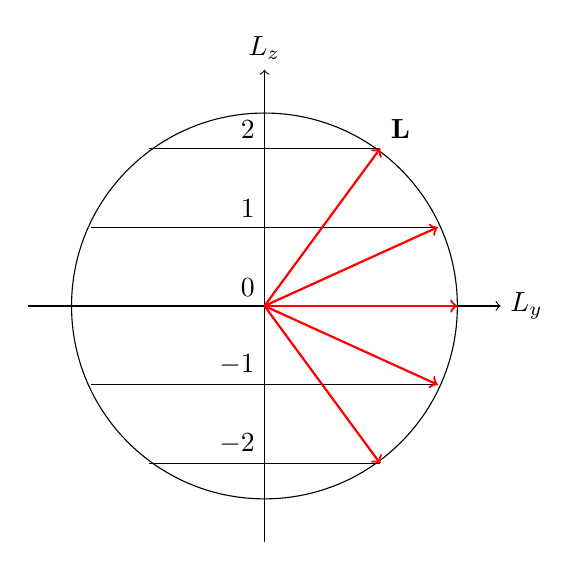
\begin{tikzpicture}
    \draw [->] (0,-3) -- (0,3);
    \draw [->] (-3,0) -- (3,0);
    \draw (0,0) circle [radius=2.45];
    \draw (-1.47,2) -- (1.47,2);
    \draw (-2.2,1) -- (2.2,1);
    \draw (-1.47,-2) -- (1.47,-2);
    \draw (-2.2,-1) -- (2.2,-1);
    \draw [thick, red, ->] (0,0) -- (1.47,2);
    \draw [thick, red, ->] (0,0) -- (2.2,1);
    \draw [thick, red, ->] (0,0) -- (2.45,0);
    \draw [thick, red, ->] (0,0) -- (1.47,-2);
    \draw [thick, red, ->] (0,0) -- (2.2,-1);
    \node [above left] at (0,2)  {$2$};
    \node [above left] at (0,1)  {$1$};
    \node [above left] at (0,0)  {$0$};
    \node [above left] at (0,-1)  {$-1$};
    \node [above left] at (0,-2) {$-2$};
    \node [above] at (0,3) {$L_z$};
    \node [right] at (3,0) {$L_y$};
    \node [above right] at (1.48, 2) {$\mathbf{L}$};
  \end{tikzpicture}
  \caption{Angular momentum startes for $l=2$.}
  \label{fig:4-3}
\end{figure}
The red arrows are supposed to represent possible angular momenta --- in units of $\hbar$ where they all have same length $\sqrt{l \left( l+1 \right)}$ and their $z$ components are allowed values of $m=-2,-1,0,1,2$.
Notice that the magnitude of the vectors is greater than the maximum $z$ component\footnote{In general, $\sqrt{l \left( l+1 \right)} > l$, except for the ``trival'' case $l=0$.}.
Evidently, you can not get the angular momentum to point perfectly along the $z$ direction.
Since to do this, you have to know all thee components simutaneously($L_x=L_y=0, L_z = \sqrt{l \left( l+1 \right)}$), and the uncertainty priciple tell us that is impossible.
It is not merely that you don't know all three components of $\mathbf{L}$; there simply aren't three components---a particle just cannot have a determinate angular momentum vector, any moer than it can simultaneously have a determinate position and moemntum.
If $L_z$ has a well-defined value, the $L_x$ and $L_y$ do not.

So, by purely algebraic means, starting with the fundamental commutation relations for angular momentum Eq.~\eqref{eq:4-69}, we have determined the eigenvalues of $L^2$ and $L_z$---without ever seeing the eigenfunctions themselves!
For the eigenfunctions, $f_l^m=Y_l^m$---the eigenfunctions of $L^2$ and $L_z$ are noting but the old sperical harmoincs function in Eq.~\eqref{eq:4-20}.
Since they are eigenfunctions of hermitian operators, $L^2$ and $L_z$, belonging to distinct eigenvalues.

\subsection{Eigenfunctions}
First, we rewrite the angular momentum in sperical coordinates, since $\mathbf{L} = \frac{\hbar}{i} \left( \mathbf{r} \times \nabla \right)$, and the gradient
\begin{equation}
  \label{eq:4-86}
  \nabla = \hat{r} \frac{\partial}{\partial r} + \hat{\theta} \frac{1}{r} \frac{\partial}{\partial \theta} + \hat{\phi} \frac{1}{r\sin\theta} \frac{\partial}{\partial \phi}
\end{equation}
meanwhile, $\mathbf{r}= r \hat{r}$, so
\begin{equation}
  \label{eq:4-87}
  \mathbf{L} = \frac{\hbar}{i} \left( \hat{\phi} \frac{\partial}{\partial \theta} - \hat{\theta} \frac{1}{\sin \theta} \frac{\partial}{\partial \phi} \right) .
\end{equation}
The unit vectors $\hat{\theta}$ and $\hat{\phi}$ can be resolved into their cartesian components due to Fig.~\ref{fig:4-1}
\begin{align}
  \label{eq:4-88}
  \hat{\theta} &= \left( \cos\theta \cos\phi \right) \hat{x} + \left( \cos\theta \sin\phi \right) \hat{y} - \left( \sin\theta \right) \hat{z} \\
  \label{eq:4-49}
  \hat{\phi} &= -\left( \sin\phi \right) \hat{x} + lr(\cos\phi) \hat{y}
\end{align}
Thus we have
\begin{align}
  \label{eq:4-90}
  L_x &= \frac{\hbar}{i} \left( -\sin\phi \frac{\partial}{\partial \theta} - \cos\phi \cot \theta \frac{\partial}{\partial \phi} \right),\\
  \label{eq:4-91}
  L_y &= \frac{\hbar}{i} \left( +\cos\phi \frac{\partial}{\partial \theta} - \sin\phi \cot \theta \frac{\partial}{\partial \phi} \right),\\
  \label{eq:4-92}
  L_z &= \frac{\hbar}{i} \frac{\partial}{\partial \phi}.
\end{align}
For descending and increasing operators
\begin{equation}
  \label{eq:4-93}
  L_{\pm} = \pm \hbar e^{\pm \phi} \left( \frac{\partial}{\partial \theta} \pm i \cot \theta \frac{\partial}{\partial \phi} \right).
\end{equation}
and $L^2$,
\begin{equation}
  \label{eq:4-94}
  L^2 = -\hbar^2 \left[ \frac{1}{\sin\theta} \frac{\partial}{\partial \theta} \left( \sin\theta \frac{\partial}{\partial \theta} \right) + \frac{1}{\sin^{2} \theta} \frac{\partial^{2}}{\partial \phi^{2}} \right] .
\end{equation}

We are now in a position to determine $f_l^m \left( \theta,\phi \right)$.
It's an eigenfunction of $L^2$, with eigenvalue $\hbar^2 l \left( l+1 \right)$.
This is precisely the angular equation, Eq.~\eqref{eq:4-9}.
And it is also an eigenfunction of $L_z$, with the eigenvalue $m\hbar$.
This is equivalent to the azimuthal equation Eq.~\eqref{eq:4-11}.
So the conclusion is the following: Spherical harmonics functions are eigenfunctions of $L^2$ and $L_z$.
When we solved the Sch\"dinger equation by separation of variables, we were inadvertently constructing simultaneous eigenfunction of the three commuting operators $H$, $L^2$, and $L_z$.

At last, there is a curious final twist to this story, for the algebraic theory of angular momentum permits $l$ to take on \textit{half-integer} values in Eq.~\eqref{eq:4-85}, whereas separation of variables yielded eigenfunctions only for \textit{integer} values in Eq.~\eqref{eq:4-17}.
n the following section, we will see the profound importance for the half-integer solutions.

\section{Spin}
In classical mechanics, a rigid object admits two kinds of angular momentum: \textbf{orbital}, associated with the motion of the center of mass, and \textbf{spin}, associated with motion about the center of mass.
For quantum mechanics, in addition to orbital angular momentum, associated with the motion of the electron around the nucleus(described by spherical harmonics in hydrogen), the electron also carries another form of angular momentum, which has nothing to do with motion in space.
The electron is a structureless point particle, and its spin angular momentum cannot be decomposed into  orbital angular momenta of constituent part.
Suffice it to say that elementary particles carry \textbf{intrinsic} angular momentum in addition to their ``extrinsic'' angular momentum.

The \textit{algebraic} theory of spin is a carbon copy of the theory of orbital angular momentum, beginning with the fundamental commutation relation
\begin{equation}
  \label{eq:4-95}
  \left[ S_i, S_j \right] = i\hbar S_k .
\end{equation}
It follows that the eigenvectors of $S^2$ and $S_z$ satisfy
\begin{equation}
  \label{eq:4-96}
  S^2 \ket{sm} = \hbar^2 s \left( s+1 \right) \ket{sm}; ~ ~ ~ S_z \ket{sm} = \hbar m \ket{sm};
\end{equation}
and
\begin{equation}
  \label{eq:4-97}
  S_{\pm} \ket{sm} = \hbar \sqrt{s \left( s+1 \right) - m \left( m \pm 1 \right)} \ket{s \left(m \pm 1 \right)} ,
\end{equation}
where $S_{\pm} \equiv S_x \pm i S_y$.
But this time the eigenvectors are not spherical harmonics(they are not functions of $\theta$ and $\phi$ at all), and there is no a \textit{priori} reason to exclude the half-integer values of $s$ and $m$
\begin{equation}
  \label{eq:4-98}
  s = 0, \frac{1}{2}, 1, \frac{3}{2}, \ldots ; ~ ~ ~  m=-s, -s+1, \ldots, s-1, s.
\end{equation}

It so happens that every elementary particle has a specific and immutable value of $s$, which we call \textbf{the spin} of the particular species: pi mesons have spin $0$; electron have spin $\frac{1}{2}$; photons have spin $1$; deltas have spin $\frac{3}{2}$; gravitions have spin  $2$; and so on.
By contrast, the orbital angular momentum quantum number $l$ can take on any integer value, and will change from one to another when the system is perturbed.
But $s$ is fixed, for any given particle, and this makes the theory of spin comparatively simple.

\subsection{Spin $\frac{1}{2}$}
By far the most important case is $s= \frac{1}{2}$, for this is the spin of the particles taht make up ordinary matter (protons, neutrons, and electrons), as well as all quarks and all leptons.
There are just two eigenstates which we call it \textbf{spin up} $\ket{ \frac{1}{2} \equiv \uparrow}$ and \textbf{spin down} $\ket{ - \frac{1}{2} \equiv \downarrow}$.
Using the basis vectors the general state of a spin-$\frac{1}{2}$ particle can be expressed as a two-element column spinor
\begin{equation}
  \label{eq:4-99}
  \chi =
  \begin{pmatrix}
    a \\
    b
  \end{pmatrix}
  =a \chi_+ + b \chi_-,
\end{equation}
with
\begin{equation}
  \label{eq:4-100}
  \chi_+ =
  \begin{pmatrix}
    1\\
    0
  \end{pmatrix}, ~ ~ ~
  \chi_- =
  \begin{pmatrix}
    0\\
    1
  \end{pmatrix}
\end{equation}
representing spin up and spin down.

Meanwhile, the spin operators become $2\times 2$ matrices.
From Eq.~\eqref{eq:4-96}, we known for $S^2$,
\begin{equation}
  \label{eq:4-101}
  S^2 \chi_{\pm}= \frac{3}{4} \hbar^2 \chi_{\pm}, ~ ~ ~
  S^2 = \frac{3}{4} \hbar^2
  \begin{pmatrix}
    1 & 0 \\
    0 & 1
  \end{pmatrix}.
\end{equation}
Similarly, for $S_z$ we have
\begin{equation}
  \label{eq:4-102}
  S_z \chi_{\pm} = \pm \frac{\hbar}{2} \chi_{\pm}, ~ ~ ~
  S_z = \frac{\hbar}{2}
  \begin{pmatrix}
    1 & 0 \\
    0 & 1
  \end{pmatrix}.
\end{equation}

Consider the properties of ladder operators, we have
\begin{equation}
  \label{eq:4-103}
  S_+ = \hbar
  \begin{pmatrix}
    0 & 1 \\
    0 & 0
  \end{pmatrix}
  , ~ ~ ~
  S_- = \hbar
  \begin{pmatrix}
    0 & 0 \\
    1 & 0
  \end{pmatrix}.
\end{equation}
Since $S_{\pm} =S_x \pm i S_y$, we have
\begin{equation}
  \label{eq:4-104}
  S_x = \frac{\hbar}{2}
  \begin{pmatrix}
    0 & 1 \\
    1 & 0
  \end{pmatrix}, ~ ~ ~
  S_y = \frac{\hbar}{2}
  \begin{pmatrix}
    0 & -i \\
    i & 0
  \end{pmatrix}.
\end{equation}
To make it tidier, we may write $\mathbf{S} = \frac{\hbar}{2} \mathbf{\sigma}$, where
\begin{equation}
  \label{eq:4-105}
  \sigma_x \equiv
  \begin{pmatrix}
    0 & 1\\
    1 & 0
  \end{pmatrix}
  , ~ ~ ~
  \sigma_y \equiv
  \begin{pmatrix}
    0 & -i \\
    i & 0
  \end{pmatrix}
  , ~ ~ ~
  \sigma_z \equiv
  \begin{pmatrix}
    1 & 0 \\
    0 & -1
  \end{pmatrix}.
\end{equation}
These are the famous \textbf{Pauli spin matrices}.
Notice that $S_x$, $S_y$, $S_z$, and $S^2$ are all hermitian.
On the other hand, $S_{\pm}$ are not hermitian.

The eigenstates of $S_z$ are
\begin{equation}
  \label{eq:4-106}
  \chi_+=
  \begin{pmatrix}
    1 \\
    0
  \end{pmatrix}
  , ~ ~ ~
  \chi_-=
  \begin{pmatrix}
    0 \\
    1
  \end{pmatrix}.
\end{equation}
If you measure $S_z$ on a particle in the geaneral state $\chi$ in Eq.~\eqref{eq:4-99}, you could get $+ \frac{\hbar}{2}$ with probabilty $\abs{a}^{2}$ and $- \frac{\hbar}{2}$ with probability $\abs{b}^{2}$.

If you measure $S_x$, then, what are the possible result and their probabilities?
First, we need to know the eigenvalues and eigenstates of $S_x$.
The characteristic equation is nothing but
\begin{equation*}
  \begin{vmatrix}
    -\lambda & \frac{\hbar}{2} \\
    \frac{\hbar}{2} & -\lambda
  \end{vmatrix}
  = 0  \to \lambda = \pm \frac{\hbar}{2}.
\end{equation*}
The normalized eigenstates of $S_x$ are
\begin{equation}
  \label{eq:4-107}
  \chi_+^x =
  \begin{pmatrix}
    \frac{1}{\sqrt{2}}\\
    \frac{1}{\sqrt{2}}
  \end{pmatrix}, ~ ~ ~
  \chi_-^x =
  \begin{pmatrix}
    \frac{1}{\sqrt{2}}\\
    - \frac{1}{\sqrt{2}}
  \end{pmatrix}.
\end{equation}
The generic spinor Eq.~\eqref{eq:4-99} can be expressed as a linear combination.

\subsection{Electron in a magnetic field: Basic}
A spinning charged particle constitutes a magnetic dipole.
Its \textbf{magnetic dipole momentum} $\mu$ is proportional to its spin angular momentum
\begin{equation}
  \label{eq:4-108}
 \boldsymbol{\mu} = \gamma \mathbf{S}
\end{equation}
the proportionality constant $\gamma$ is called the \textbf{gyromagnetic ratio}.
With a magnetic field $\mathbf{B}$, it experiences a torque, $\boldsymbol{\mu} \times \mathbf{B}$, which tends to line it up parallel to the field.
The energy associated with this torque is
\begin{equation}
  \label{eq:4-109}
 H = - \boldsymbol{\mu} \cdot \mathbf{B},
\end{equation}
so the Hamiltonian of a spinning charged particle, at rest\footnote{If a particle is allowed to move, there will be kinetic energy and Lorentz force, which is not derivable from a potential energy function and hence does not fit the Schr\"odinger equation as we formulated so far.} in a magnetic field $\mathbf{B}$ is
\begin{equation}
  \label{eq:4-110}
  H = - \gamma \mathbf{B} \cdot \mathbf{S}.
\end{equation}

\subsection{Larmor precession}
Imagine a particle of spin $\frac{1}{2}$ at rest in a uniform magnetic field, which points in the $z$-direction
\begin{equation}
  \label{eq:4-111}
 \mathbf{B} = B_0 \hat{z}.
\end{equation}
The Hamiltonian in matrix form is
\begin{equation}
  \label{eq:4-112}
 H = - \gamma B_0 S_z = - \frac{\gamma B_0 \hbar}{2}
 \begin{pmatrix}
   1 & 0 \\
   0 & 1
 \end{pmatrix}.
\end{equation}
The eigenstate of this $H$ are the same as those of $S_z$ in Eq.~\eqref{eq:4-106} with energy $E_{\pm} = \mp \frac{\gamma B_0 \hbar}{2}$.

Since the Hamiltonian is time-independent, the general solution the the time-dependent Schr\"odinger equation, $i\hbar \frac{\partial \chi }{\partial t} = H \chi$, can be expressed in terms of stationary states
\begin{equation*}
  \chi \left( t \right) =
  \begin{pmatrix}
    \cos \left( \frac{\alpha}{2} \right) e^{i\gamma B_0 t/2} \\
    \sin \left( \frac{\alpha}{2} \right)  e^{-i \gamma B_0 t/2}
  \end{pmatrix}.
\end{equation*}
The constants $\cos \left( \frac{\alpha}{2} \right)$ and $\sin \left( \frac{\alpha}{2} \right)$ are determined by the initial condition and the physical importance of the phase angle $\alpha$ will discussed later.

One can calculate the expectation value of $\mathbf{S}$ as a function of time
\begin{align}
  \label{eq:4-113}
 \expval{S_x} &= \chi \left( t \right)^{\dagger} S_x \chi \left( t \right) = \frac{\hbar}{2} \sin \alpha \cos \left( \gamma B_0 t \right) \\
  \label{eq:4-114}
 \expval{S_y} &= \chi \left( t \right)^{\dagger} S_y \chi \left( t \right) = \frac{\hbar}{2} \sin \alpha \sin \left( \gamma B_0 t \right) \\
  \label{eq:4-115}
 \expval{S_z} &= \chi \left( t \right)^{\dagger} S_z \chi \left( t \right) = \frac{\hbar}{2} \cos \alpha
\end{align}
Evidently $\expval{\mathbf{S}}$ is tilted at a constant angle $\alpha$ to the $z$-axis, and precesses about the field at the \textbf{Larmor frequency}
\begin{equation}
  \label{eq:4-116}
 \omega = \gamma B_0,
\end{equation}
just as it would classically.
This is because the Ehrenfest's theorem guarantees that $\expval{\mathbf{S}}$ evolves according to the classical laws.

For example, the \textbf{Stern-Gerlach experiment} is an application of this effect as shwon in Fig.~\ref{fig:4-4}.
In an \textit{inhomogeneous} magnetic field, there is not only a \textit{torque}, but also a force on a magnetic dipole\footnote{We assume a neutral particle to avoid the Lorentz force and heavy so we can construct localized wave packets and treat the motion in terms of classical particle trajectories. In practice, the Stern-Gerlach experiment does not work, for example, with a beam of free electrons.}
\begin{equation}
  \label{eq:4-117}
 \mathbf{F} = \nabla \left( \boldsymbol{\mu} \cdot \mathbf{B} \right) .
\end{equation}
This force can be used to separate out particles with a particular spin orientation.
Imagine a beam of relatively heavy neutral atom which pass through a region of inhomogeneous magnetic field
\begin{equation}
  \label{eq:4-118}
 \mathbf{B} \left( x,y,z \right) = -\alpha x \hat{x} + \left( B_0 + \alpha z \right) \hat{z}
\end{equation}
where $B_0$ is a strong uniform field and the constant $\alpha$ describes a small deviation from homogeneity\footnote{We can not have something only with $z$ component in this case, since it breaks the electromagnetic law $\nabla \cdot \mathbf{B} = 0$.}.

\begin{figure}[t]
  \centering
  \includegraphics[width=0.75\textwidth]{fig/fig4-3.png}
  \label{fig:4-4}
  \caption{The setup of Stern-Gerlach experiment. (1) source; (2) hole; (3) inhomogeneous magnetic field; (4) the classical expectation and (5) the observation.}
\end{figure}

The corresponding force on the atom is
\begin{equation*}
  \mathbf{F} = \gamma \alpha \left( -S_x \hat{x} + S_z \hat{z} \right) .
\end{equation*}
However, as Eq.~\eqref{eq:4-113} suggested, due to the Larmor precession about $B_0$, $S_x$ oscillates rapidly and averages to zero.
The \textit{net} force is purely in the $z$ direction
\begin{equation}
  \label{eq:4-119}
 F_z = \gamma \alpha S_z
\end{equation}
and the beam is deflected up or down, in proportion to the $z$ component of the spin angular momentum.

In the more \textit{quantum} argument, we examine the process from the perspective of a reference frame that moves along with the beam.
In this frame the Hamiltonian starts out zero, turns on for a time $T$ and then turn off again
\begin{equation}
  \label{eq:4-120}
  H \left( t \right) =
  \begin{cases}
    0,~ ~ ~ &\text{for $t<0$} \\
    -\gamma \left( B_0 + \alpha a \right) S_z, ~ ~ ~ &\text{for $0\leq t \leq T$}\\
    0,~ ~ ~  &\text{for $t>T$}
  \end{cases},
\end{equation}
where we have ignore the $x$ component contribution from $\mathbf{B}$ for the same reason discussed before.
Suppose the atom has spin $\frac{1}{2}$ and starts out in the state
\begin{equation*}
\chi(t) = a \chi_+ + b \chi_- ~ ~ ~ \text{for $t\leq 0$}.
\end{equation*}
In the magnetic filed region where the non-zero Hamiltonian acts, we have
\begin{equation*}
\chi \left( t \right) = a \chi_+ e^{-i E_+ t/hbar} + b \chi_- e^{-iE_-t/\hbar} ~ ~ ~ \text{for $0\leq t \leq T$},
\end{equation*}
where
\begin{equation}
  \label{eq:4-121}
  E_{\pm} = \mp \gamma \left( B_0 +\alpha z \right) \frac{\hbar}{2}
\end{equation}
and hence it emerges in the state
\begin{equation}
  \label{eq:4-122}
  \chi \left( t \right) = \left( a e^{i\gamma T B_0/2} \chi_+ \right) e^{i \left( \alpha \gamma T/2 \right)z} + \left( b e^{-i\gamma T B_0/2} \chi_- \right) e^{-i \left( \alpha \gamma T/2 \right)z}.
\end{equation}
The two terms now carry \textit{momentum} in the $z$ direction
\begin{equation}
  \label{eq:4-123}
 p_z = \pm \frac{\alpha \gamma T \hbar}{2}.
\end{equation}
Thus $\chi_+$ will moves in the plus-$z$ direction and opposite for $\chi_-$ state.

\subsection{Addition of angular momenta}
Suppose now that we have two spin-$\frac{1}{2}$ particles---for example, the electron and the proton in the ground state of hydrogen.
Each can have spin up or spin down, so there are four possibilities in all\footnote{We consider the ground state, so there  will not any orbital angular momentum to worry about.}
\begin{equation}
  \label{eq:4-124}
 \ket{\uparrow \uparrow}, ~ \ket{\uparrow \downarrow},~ \ket{\downarrow \uparrow}, ~ \ket{\downarrow \downarrow},
\end{equation}
where the first arrow refer to the electron and the second to the proton.
We want to know what is the total angular momentum of the atom $\mathbf{S} \equiv \mathbf{S}_1 + \mathbf{S}_{2}$.
Since each of these four composite states in Eq.~\eqref{eq:4-124}, is an eigenstate of $S_z$, we have
\begin{equation*}
  S_z\ket{\chi_1 \chi_2} = \left( S_1 + S_2 \right) \ket{\chi_1 \chi_2} = \hbar \left( m_1 + m_2 \right) \ket{\chi_1 \chi_2}
\end{equation*}
So $m$ is just $m_1+m_2$:
\begin{align*}
  m &=1 ~ ~ ~ \ket{\uparrow \uparrow}\\
  m &=0 ~ ~ ~ \ket{\uparrow \downarrow}\\
  m &=0 ~ ~ ~ \ket{\downarrow \uparrow}\\
  m &=-1 ~ ~ ~ \ket{\downarrow \downarrow}.
\end{align*}

At first glance, this does not look right: $m$ is suppose to advance in integer steps from $-s$ to $+s$ where $s=1$ in our case.
However, there is an ``extra'' state with $m=0$.
One way to untangle this problem is to apply the lowering operator to the state $\ket{\uparrow \uparrow}$
\begin{equation*}
  S_- \ket{\uparrow \uparrow} = \hbar \left( \ket{\downarrow \uparrow} + \ket{\uparrow \downarrow} \right).
\end{equation*}
Evidently, in the notation of $\ket{sm}$, the three stats with $s=1$ are
\begin{equation}
  \label{eq:4-125}
  s = 1 ~ \text{(triplet state)} ~ \to
  \begin{cases}
    \ket{11} &= \ket{\uparrow \uparrow} \\
    \ket{10} &= \frac{1}{\sqrt{2}} \left( \ket{\uparrow \downarrow} + \ket{\downarrow \uparrow} \right)\\
    \ket{1-1} &= \ket{\downarrow \downarrow}
  \end{cases}.
\end{equation}
This is called the \textbf{triplet} combination.
Meanwhile, the orthogonal state with $m=0$ carries $s=0$
\begin{equation}
  \label{eq:4-126}
  s = 0 ~ \text{(singlet state)} ~ \to \ket{00} = \frac{1}{\sqrt{2}} \left( \ket{\uparrow\downarrow} - \ket{\downarrow \uparrow} \right).
\end{equation}

We found that the combination of two spin-$\frac{1}{2}$ particles can carry a total spin of $1$ and $0$, depending on whether they occupy the triplet or the single configuration.
To verify this, we will prove that the triplet states are eigenvectors of $S^2$ with eigenvalue $\hbar^{2} s \left( s+1 \right) = 2\hbar^{2}$ and single is for eigenvalue $0$.
Now,
\begin{equation}
  \label{eq:4-127}
 S^2 = \left( \mathbf{S}_1 + \mathbf{S}_2 \right) \cdot \left( \mathbf{S}_1 + \mathbf{S}_2 \right) = S_1^2 + S_2^2 + 2 \mathbf{S}_1 \cdot \mathbf{S}_2.
\end{equation}
Using Eq.~\eqref{eq:4-102} and Eq.~\eqref{eq:4-104}, we have
\begin{align*}
  & \mathbf{S}_1 \cdot \mathbf{S}_2 \ket{\uparrow \downarrow} \\
  =& \left( S_{x1}S_{x2} + S_{y1}S_{y2} + S_{z1}S_{z2} \right) \ket{\uparrow\downarrow}\\
  =& \frac{\hbar^{2}}{4} \left( 2\ket{\downarrow\uparrow} - \ket{\uparrow\downarrow} \right).
\end{align*}
Similarly,
\begin{equation*}
   \mathbf{S}_1 \cdot \mathbf{S}_2 \ket{\downarrow \uparrow}  =  \frac{\hbar^{2}}{4} \left( 2 \ket{\uparrow \downarrow} - \ket{\downarrow\uparrow} \right).
\end{equation*}
Then returning to Eq.~\eqref{eq:4-125}, we have
\begin{equation}
  \label{eq:4-128}
  S^2 \ket{10} = \left( \frac{3\hbar^{2}}{4} + \frac{3\hbar^{2}}{4} + 2 \frac{\hbar^{2}}{4} \right) \ket{10} = 2\hbar^2 \ket{10},
\end{equation}
so $\ket{10}$ is indeed an eigenstate of $s^2$ with eigenvalue $2\hbar^{2}$.
We can did the similar calculation for $\ket{00}$ and we have $S^2 \ket{00}= 0 \ket{00}$.

This is the simplest example of a larger problem: If you combine spin $s_1$ with spin $s_2$, the total spins $s$ you can get is
\begin{equation}
  \label{eq:4-129}
 s = \left( s_1 + s_2 \right), \left( s_1+s_2-1 \right), \ldots, \abs{s_1-s_2},
\end{equation}
where they are in integer steps.
For example, if you package together a particle of spin $\frac{3}{2}$ with a particle of spin $2$, you could get a total spin of $\frac{7}{2}$, $\frac{5}{2}$, $\frac{3}{2}$, or $\frac{1}{2}$, depending on the configuration.
Another example, if a hydrogen atom is in the state $\psi_{nlm}$, the net angular momentum of the electron is $l+ \frac{1}{2}$ or $l - \frac{1}{2}$;
if you now throw in a \textit{proton}, the atom's total angular momentum quantum number is $l+1$, $l$, or $l-1$.

The combined state $\ket{sm}$ with total spin $s$ ans $z$-component $m$ will be some linear combination of the composite states $\ket{s_1 m_1}\ket{s_2 m_2}$:
\begin{equation}
  \label{eq:4-130}
 \ket{sm}  = \sum_{m_1+m_2=m} C_{m_1m_2m}^{s_1s_2s} \ket{s_1 m_1} \ket{s_2 m_2}.
\end{equation}
The constants $C_{m_1m_2m}^{s_1s_2s}$ are called \textbf{Clebsch-Gordan coefficients}
The simplest case are listed in Fig.~\ref{fig:4-5}.
\begin{figure}[t]
  \centering
  \includegraphics[width=0.95\textwidth]{fig/fig4-4.png}
  \label{fig:4-5}
  \caption{Clebsch-Gordan coefficients. A square root sign is understood for every entry; the minus sign, if present, goes outside the radical.}
\end{figure}
For example, the shaded column of $2\times 1$ table tell us that
\begin{equation*}
\ket{30} = \frac{1}{\sqrt{5}}\ket{21}\ket{1-1} + \sqrt{\frac{3}{5}}\ket{20}\ket{10} + \frac{1}{\sqrt{5}}\ket{2-1}\ket{11}.
\end{equation*}
In particular, if two particles (of spin $2$ and spin $1$) are at rest in a box, and the total spin is $3$, and its $z$ component is $0$ (where $\ket{30}$), then a measurement of $S_z^1$ could return the value $\hbar$ (with probability $\frac{1}{5}$), or $0$ (with probability $\frac{3}{5}$), or $-\hbar$ (with probability $\frac{1}{5}$).

These tables also work the other way around
\begin{equation}
  \label{eq:4-131}
 \ket{s_1 m_1} \ket{s_2 m_2} = \sum_s C_{m_1m_2m}^{s_1s_2s} \ket{sm}.
\end{equation}
For example, the shaded row in the $\frac{3}{2}\times 1$ table tells us that
\begin{equation*}
  \ket{\frac{3}{2} \frac{1}{2}} \ket{10} = \sqrt{\frac{3}{5}} \ket{\frac{5}{2} \frac{1}{2}} + \sqrt{\frac{1}{15}} \ket{\frac{3}{2} \frac{1}{2}} - \sqrt{\frac{1}{3}} \ket{\frac{1}{2} \frac{1}{2}}
\end{equation*}
If you put particles of spin $\frac{3}{2}$ and spin $1$ in the box, and you know that the first has $m_1= \frac{1}{2}$ and the second has $m_2=0$, and you measure the total spin, $s$, you could get $\frac{5}{2}$ (with probability $\frac{3}{5}$), or $\frac{3}{2}$ (with probability $\frac{1}{15}$), or $\frac{1}{2}$ (with probability $\frac{1}{3}$).

In a mathematical sense this is all applied \textbf{group theory}---what we are talking about is the decomposition of the direct product of two irreducible representations of the rotation group into a direct sum of irreducible representations.










%%% Local Variables:
%%% mode: latex
%%% TeX-master: "main"
%%% End:

\chapter{Identical particles}

\section{Two-particle system}
For a single particle, $\Psi \left( \mathbf{r},t \right)$ is a function of the spatial coordinate and time (we will ignore spin).
For two-particle system the wave function is $\Psi \left( \mathbf{r}_1, \mathbf{r}_2, t \right)$.
It evolves with the Schr\"odinger equation with the Hamiltonian
\begin{equation}
  \label{eq:5-1}
 H = - \frac{\hbar^{2}}{2m_{1}} \nabla_1^2 - \frac{\hbar^{2}}{2m_{2}} \nabla_2^2 + V \left( \mathbf{r}_1,\mathbf{r}_2,t \right).
\end{equation}

Typically, the interaction potential depends only the vector $\mathbf{r} \equiv \mathbf{r}_1 - \mathbf{r}_2$ between the two particles.
We can change the variable to $\mathbf{r}$ and $\mathbf{R} \equiv \frac{m_{1} \mathbf{r}_1 + m_2 \mathbf{r}_2}{m_1+m_2}$.
Relate to the old coordinate, we have $\mathbf{r}_{1,2} = \mathbf{R} \pm \mathbf{r} \frac{\mu}{m_{1,2}}$, and $\nabla_{1,2} = \frac{\mu}{m_{2,1}} \nabla_R \pm \nabla_{r}$ where
\begin{equation}
  \label{eq:5-2}
 \mu \equiv \frac{m_1 m_2}{m_1 + m_2}
\end{equation}
is the \textbf{reduced mass} of the system.
The Shr\"odinger equation becomes
\begin{equation}
  \label{eq:5-3}
 - \frac{\hbar^{2}}{2 \left( m_1 + m_2 \right)}  \nabla^2_R \psi - \frac{\hbar^{2}}{2\mu} \nabla^2_r \psi + V \left( \mathbf{r} \right) \psi = E\psi.
\end{equation}
We can further separate the variables, $\psi \left( \mathbf{R}, \mathbf{r} \right) = \psi_R \left( \mathbf{R} \right) \psi_r \left( \mathbf{r} \right)$ to see that they are two single particle problem.

\subsection{Bosons and Fermions}
Suppose there are two particles and they can be represented in the way of simple product\footnote{In \textbf{entangled states}, you can not decomposed in that way. If particle one is in state $a$ and particle two is in state $b$, then the two-particle state is a product. The simplest example of entangled state is the singlet spin configuration in Eq.~\eqref{eq:4-126}. You can not tell the state of particle one by itself, because it is ``entangled'' with the state of particle two. If $2$ is measured, and found to be spin up, then $1$ is spin down, but if $2$ is spin down, then $1$ is spin up.}
\begin{equation}
  \label{eq:5-4}
  \psi \left( \mathbf{r}_1, \mathbf{r}_2 \right)  = \psi_a \left( \mathbf{r}_1 \right) \psi_b \left( \mathbf{r}_2 \right).
\end{equation}
Of course, this assumes that we can tell the particles apart---otherwise it wouldn't make any sense to claim that number $1$ is in state $\psi_a$ and number $2$ is in state $\psi_b$; all we could say is that one of them is in the state $\psi_a$ and the other is in state $\psi_b$, but we wouldn't know which is which.
\marginnote{Some discussion from \href{https://physics.stackexchange.com/questions/405155/are-identical-particles-always-entangled-even-when-not-interacting}{stackexchange}:

Entanglement is only a meaningful concept when there is a well-defined notion of subsystems, which generally means spatially separated subsystems. Indeed, the notion of "product state" (or its converse, "entangled state") is only meaningful relative to a given tensor product decomposition of the Hilbert space, which implicitly defines a splitting into subsystems. Hence, it is not obvious that indistinguishable particles with an (anti-)symmetrised wavefunction can be truly regarded as entangled subsystems.

Nevertheless, \href{https://arxiv.org/abs/1312.4311}{Killoran, Cramer and Plenio} showed that this is indeed a genuine form of entanglement. That is, the entanglement formally associated with the symmetrised wave function of a system of indistinguishable bosons can be extracted into the equivalent amount of entanglement (asymptotically) between distinguishable modes.
I believe a similar result was found also for fermions by \href{https://arxiv.org/abs/quant-ph/0608141}{Cavalcanti et al}.
}
This is what happened, since all electrons are utterly identical unlike classical objects.

Quantum mechanics neatly accommodates the existence of particles that are \textit{indistinguishable in principle:} We simply construct a wave function that is \textit{noncommittal} as to which particle is in which state.
There are actually two ways to do it
\begin{equation}
  \label{eq:5-5}
 \psi_{\pm} \left( \mathbf{r}_1, \mathbf{r}_2 \right) = A \left[ \psi_a \left( \mathbf{r}_1 \right) \psi_b \left( \mathbf{r}_2 \right) \pm \psi_b \left( \mathbf{r}_1 \right) \psi_a \left( \mathbf{r}_2 \right) \right] .
\end{equation}
Thus the theory admits two kinds of identical particles: \textbf{bosons} (plus sign with integer spin) and \textbf{fermions} (minus sign with half integer spin).
This connection between \textbf{spin and statistics} can be proved in relativistic quantum mechanics; in non-relativistic theory it is taken as an axiom.

It follows, in particular, that \textit{two identical fermions can not occupy the same state}.
This is the famous \textbf{Pauli exclusion principle}.
There is a more general way to formulate the problem.
Let us define the \textbf{exchange operator}, $P$, which interchanges the two particles:
\begin{equation}
  \label{eq:5-6}
 P f lr(r_1,r_2) = f lr(r_2,r_1) .
\end{equation}
Clearly, $P^2=1$, and it follows that the eigenvalues of $P$ are $\pm 1$.
Now, if the two particles are identical, the Hamiltonian must treat them the same: $m_1=m_2$ and $V \left( r_1,r_2 \right)=V \left( r_2,r_1 \right)$.
This suggest that $P$ and $H$ are compatible observables
\begin{equation}
  \label{eq:5-7}
  \left[ P,H \right]=0,
\end{equation}
and hence we can find a complete set of functions that are simultaneous eigenstates of both.
That is to say, we can find solutions to the Schr\"odinger equation that are either symmetric or antisymmetric under exchange:
\begin{equation}
  \label{eq:5-8}
 \psi \left( r_1, r_2 \right) = \pm \psi \left( r_2, r_1 \right) .
\end{equation}
Moreover, if a system starts our in such state, it will remain in a such state.
For identical particles the wave function is not merely \textit{allowed}, but \textit{required} to satisfy Eq.~\eqref{eq:5-8}, with the plus sign for bosons, and minus sign for fermions.

\subsection{Exchange force}
Suppose on particle is in state $\psi_a \left( x \right)$, and the other is in state $\psi_b \left( x \right)$, and these two states are orthogonal and normalized.
If the two particle are distinguishable, and number $1$ is in the state $\psi_a$, then the combined wave function is
\begin{equation}
  \label{eq:5-9}
  \psi \left( x_1,x_2 \right) = \psi_a \left( x_1 \right) \psi_b \left( x_2 \right);
\end{equation}
if they are identical particles, the composite wave function is
\begin{equation}
  \label{eq:5-10}
 \psi_{\pm} \left( x_1,x_2 \right) = \frac{1}{\sqrt{2}} \left[ \psi_a \left( x_1 \right) \psi_b \left( x_2 \right) \pm \psi_b \left( x_1 \right) \psi_a \left( x_2 \right) \right].
\end{equation}
We will calculate the expectation value of the square of the separation distance between the two particles,
\begin{equation}
  \label{eq:5-11}
 \expval{\left( x_1 - x_2 \right)^2} = \expval{x_1^2} + \expval{x_2^2} - 2\expval{x_1x_2}.
\end{equation}

\textbf{Case 1: Distinguishable particles}. For the wavefunction in Eq.~\eqref{eq:5-9},
\begin{equation*}
  \expval{ x_1^2 } = \int x_1^2 \abs{ \psi_a \left( x_1 \right) }^2 \dd x_1 \int \abs{\psi_b \left( x_2 \right)} \dd x_{2} = \expval{x^2}_{a}
\end{equation*}
With similar procedure, we have the result:
\begin{equation}
  \label{eq:5-12}
   \expval{\left( x_1 - x_2 \right)^2}_d = \expval{x_1^2}_a + \expval{x_2^2}_b - 2\expval{x_1}_a\expval{x_2}_b.
\end{equation}

\textbf{Case 2: Identical particles.} For the wave function in Eq.~\eqref{eq:5-10},
\begin{align*}
  \expval{x_1^2} &= \frac{1}{2} \Big[ \int x_1^2 \abs{ \psi_a \left( x_1 \right) }^2 \dd x_1 \int \abs{\psi_b \left( x_2 \right)} \dd x_{2}\\
                 &+  \int x_1^2 \abs{ \psi_b \left( x_1 \right) }^2 \dd x_1 \int \abs{\psi_a \left( x_2 \right)} \dd x_{2}\\
                 &\pm \int x_1^2 \psi_a \left( x_1 \right)^{*} \psi_b \left( x_1 \right) \dd x_1 \int \psi_b \left( x_2 \right)^{*} \psi_a \left( x_2 \right) \dd x_{2}\\
                 &\pm \int x_1^2 \psi_b \left( x_1 \right)^{*} \psi_a \left( x_1 \right) \dd x_1 \int \psi_a \left( x_2 \right)^{*} \psi_b \left( x_2 \right) \dd x_{2} \Big] \\
                 &= \frac{1}{2} \left[ \expval{x^2}_a + \expval{x^2}_b \pm 0 \pm 0 \right]
\end{align*}
Since particle are identical you can not tell them apart, we have same result for $\expval{x_2^{2}}$.
But for the rest part,
\begin{align*}
  \expval{x_1 x_2} &= \frac{1}{2} \Big[ \int x_1 \abs{ \psi_a \left( x_1 \right) }^2 \dd x_1 \int x_2 \abs{\psi_b \left( x_2 \right)} \dd x_{2}\\
                   &+  \int x_1 \abs{ \psi_b \left( x_1 \right) }^2 \dd x_1 \int x_2 \abs{\psi_a \left( x_2 \right)} \dd x_{2}\\
                   &\pm \int x_1 \psi_a \left( x_1 \right)^{*} \psi_b \left( x_1 \right) \dd x_1 \int x_2 \psi_b \left( x_2 \right)^{*} \psi_a \left( x_2 \right) \dd x_{2}\\
                   &\pm \int x_1 \psi_b \left( x_1 \right)^{*} \psi_a \left( x_1 \right) \dd x_1 \int x_2 \psi_a \left( x_2 \right)^{*} \psi_b \left( x_2 \right) \dd x_{2} \Big] \\
                   &= \expval{x}_a \expval{x}_b \pm \abs{ \expval{x}_{ab} }^{2},
\end{align*}
where
\begin{equation}
  \label{eq:5-13}
 \expval{x}_{ab} \equiv \int x \psi_a \left( x \right)^{*} \psi_b \left( x \right) \dd x.
\end{equation}
Evidently, we have the result:
\begin{equation}
  \label{eq:5-14}
   \expval{\left( x_1 - x_2 \right)^2}_\pm = \expval{x_1^2}_a + \expval{x_2^2}_b - 2\expval{x_1}_a\expval{x_2}_b \mp 2 \abs{\expval{x}_{ab}}^{2}.
\end{equation}

Comparing Eq.~\eqref{eq:5-12} and Eq.~\eqref{eq:5-14}, we see that the difference resides in the final term:
\begin{equation}
  \label{eq:5-15}
 \expval{ \left( \Delta x \right)^2 }_{\pm} = \expval{ \left( \Delta x \right)^2 }_d \mp 2 \abs{ \expval{x}_{ab} }^{2}.
\end{equation}
Identical bosons tend to be somewhat closer together, and identical fermions somewhat further apart, than distinguishable particle in the same two states.
Notice that $\expval{x}_{ab}$ vanishes unless the two wave functions actually overlap.
As a \textit{practical} matter, therefore, it is okay to pretend that electrons with non-overlapping wave functions are distinguishable.

The \textit{interesting} case is when there is some overlap of the wave function.
The system behaves as through there were a ``force of attraction'' between identical bosons, pulling them closer together, and a ``force of repulsion'' between identical fermions, pushing them apart.
We call it an \textbf{exchange force}, although it is not really a force at all---no physical agency is pushing on the particles; rather, it is a purely \textit{geometrical} consequence of the symmetrization requirement.
It is also a strictly quantum mechanical phenomenon, with no classical counterpart.

There has profound consequences.
Considering the hydrogen molecule $H_{2}$.
Roughly speaking, the ground state consists of one electron in the atomic ground state, Eq.~\eqref{eq:4-53}, centered at nucleus $1$, and one electron in the atomic ground state centered at nucleus $2$.
If electrons where \textbf{bosons}, the symmetrization requirement would tend to concentrate the electrons toward the middle, between the two protons, and the resulting accumulation of negative charge  would attract the protons inward, accounting for the \textbf{covalent bound} as shown in Fig.~\ref{fig:5-1}.
Unfortunately, electron are not bosons, they are fermions, and this means that the concentration of negative charge should actually be shifted to the wings, tearing the molecule apart.
\begin{figure}[t]
  \centering
  \includegraphics[width=0.75\textwidth]{fig/fig5-1.png}
  \label{fig:5-1}
  \caption{Schematic picture of the covalent bond: (a) Symmetric configuration produce attractive force. (b) Antisymmetric configuration produce repulsive force.}
\end{figure}

However, this is the conclusion when the spin is ignored.
The complete state of the electron includes not only its position wave function, but also a spinor, describing the orientation of the spin.
When we put together the two-electron state, it is the \textbf{whole works}, not just the spatial part, that has to be antisymmetric with respect to exchange.
Now, a glance back at the composite spin states Eq.~\eqref{eq:4-125} and Eq.~\eqref{eq:4-126} reveals that the singlet combination is antisymmetric and hence would have to be joined with a symmetric spatial function, whereas the three triplet states are all symmetric and would require an antisymmetric spatial function.
Evidently, then, the singlet state should lead to \textit{binding}, and the triplet to \textit{antibonding}.
Sure enough, the chemists tell us that covalent bonding requires the two electrons to occupy the singlet state, with total spin zero.

\section{Atoms}
A neutral atom, of atomic number $Z$, consists of a heavy nucleus, with electric charge $Ze$, surrounded by $Z$ electrons.
The Hamiltonian for the system\footnote{We are assuming the nucleus is stationary. The nucleus is so much more massive than the electrons that the correction is extremely small even in the case of hydrogen and it is smaller still for the heavier atoms.}
\begin{equation}
  \label{eq:5-16}
 H = \sum_{j=1}^Z \left\{ - \frac{\hbar^{2}}{2m} \nabla^2_j - \left( \frac{1}{4\pi \epsilon_{0}} \right)  \frac{Z e^{2}}{r_{j}}\right\} + \frac{1}{2} \left( \frac{1}{4 \pi \epsilon_{0}} \right) \sum_{j \neq k}^Z \frac{e^{2}}{\abs{\mathbf{r}_j - \mathbf{r}_k}}.
\end{equation}
The term in curly brackets represents the kinetic plus potential energy of the $j$th electron, in the electric field of the nucleus; the second sum is the potential energy associated with the mutual repulsion of the electrons.
The problem is to solve Schr\"odinger's equation,
\begin{equation}
  \label{eq:5-17}
 H \psi = E \psi,
\end{equation}
for the wave function $\psi \left( \mathbf{r}_1, \ldots, \mathbf{r}_Z \right)$.
Because electrons are identical, for the complete state,
\begin{equation}
  \label{eq:5-18}
  \psi \left( \mathbf{r}_1, \ldots, \mathbf{r}_Z \right) \chi \left( \mathbf{s}_1, \ldots, \mathbf{s}_{Z} \right),
\end{equation}
should be antisymmetric with respect to interchange of any two electrons.

The Schr\"odinger equation with Hamiltonian in Eq.~\eqref{eq:5-16} can not be solved exactly.
Some qualitative features will be discussed here.

\subsection{Helium}
After the hydrogen, the simplest atom is helium ($Z=2$).
The Hamiltonian,
\begin{equation}
  \label{eq:5-19}
  H = \left\{ - \frac{\hbar^{2}}{2m} \nabla_1^2 - \frac{1}{4\pi \epsilon_{0}} \frac{2e^{2}}{r_{1}} \right\} +  \left\{ - \frac{\hbar^{2}}{2m} \nabla_2^2 - \frac{1}{4\pi \epsilon_{0}} \frac{2e^{2}}{r_{2}} \right\} + \frac{1}{4\pi\epsilon_{0}} \frac{e^{2}}{\abs{\mathbf{r}_1- \mathbf{r}_{2}}},
  \end{equation}
consists of two hydrogenic Hamiltonians.
If we simply \textit{ignore} the last interaction term, the Schr\"odinger equation separates, and the solutions can be written as products of \textit{hydrogen} wave function:
\begin{equation}
  \label{eq:5-20}
 \psi \left( \mathbf{r}_1, \mathbf{r}_2 \right) = \psi_{nlm} \left( \mathbf{r}_1 \right) \psi_{n'l'm'} \left( \mathbf{r}_2 \right) ,
\end{equation}

only with half the Bohr radius, in Eq.~\eqref{eq:4-46}, and four times the Bohr energies, in Eq.~\eqref{eq:4-44}.
The total energy would be
\begin{equation}
  \label{eq:5-21}
 E = 4 \left( E_n + E_{n'} \right) ,
\end{equation}
where $E_n = - \frac{13.6}{n^{2}}$eV.
In particular, the ground state would be
\begin{equation}
  \label{eq:5-22}
 \psi_0 \left( \mathbf{r}_1, \mathbf{r}_2 \right) =\psi_{100} \left( \mathbf{r}_1 \right) \psi_{100} \left( \mathbf{r}_2 \right) = \frac{8}{\pi a_{0}^{3}} e^{-2 \left( r_1 + r_2 \right)/a_{0}},
\end{equation}
and it energy would be $E_0 = -109$eV.
Because $\psi_0$ is a symmetric function, the spin state has to be antisymmetric, so the ground state of helium should be a \textit{singlet} configuration.
The actual ground state of helium is indeed a single but experimentally determined energy is $-78.975$eV.
This mismatch is due to the interaction from the last term of Eq.~\eqref{eq:5-16}.

The excited states of helium consist of one electron in the hydrogenic ground state, and the other in an excited state\footnote{If you try to put both electrons in excited states, one immediately drops to the ground state, releasing enough energy to knock the other one into continuum, leaving with a helium ion and a free electron.}:
\begin{equation}
  \label{eq:5-23}
 \psi_{nlm}\psi_{100}.
\end{equation}











%%% Local Variables:
%%% mode: latex
%%% TeX-master: "main"
%%% End:


\bibliography{mybib}{}
\bibliographystyle{abbrv}
\end{document}

%%% Local Variables:
%%% mode: latex
%%% TeX-master: t
%%% End:
